\documentclass[a4paper]{report}

%====================== PACKAGES ======================
\usepackage{graphicx}
\usepackage[english,french]{babel}
\usepackage[utf8x]{inputenc}
\usepackage{multirow}

%pour gérer les positionnement d'images
\usepackage{float}
\usepackage{amsmath}
\usepackage{graphicx}
\usepackage[colorinlistoftodos]{todonotes}
\usepackage{url}
%pour les informations sur un document compilé en PDF et les liens externes / internes
\usepackage{hyperref}
%pour la mise en page des tableaux
\usepackage{array}
\usepackage{tabularx}
\usepackage{dingbat}
%pour utiliser \floatbarrier
%\usepackage{placeins}
%\usepackage{floatrow}
%espacement entre les lignes
\usepackage{setspace}
%modifier la mise en page de l'abstract
\usepackage{abstract}
%police et mise en page (marges) du document
\usepackage[T1]{fontenc}
\usepackage[top=2cm, bottom=2cm, left=2cm, right=2cm]{geometry}
%Pour les galerie d'images
\usepackage{subfig}
\usepackage{titleps}
\usepackage{fancyhdr}
\newpagestyle{mine}{
\sethead[\chaptername~ \thechapter~|~\chaptertitle][][]{}{}{\thesection.~\sectiontitle}
\setfoot[\thepage][][]{}{}{\thepage}
}
\renewpagestyle{plain}{
\setfoot[\thepage][][]{}{}{\thepage}
}
%====================== INFORMATION ET REGLES ======================

%rajouter les numérotation pour les \paragraphe et \subparagraphe
\setcounter{secnumdepth}{4}
\setcounter{tocdepth}{4}

\hypersetup{							% Information sur le document
pdfauthor = {Premier Auteur,
			Deuxième Auteur,
			Troisième Auteur,
    		Quatrième Auteur},			% Auteurs
pdftitle = {Nom du Projet -
			Sujet du Projet},			% Titre du document
pdfsubject = {Mémoire de Projet},		% Sujet
pdfkeywords = {Tag1, Tag2, Tag3, ...},	% Mots-clefs
pdfstartview={FitH}}					% ajuste la page à la largueur de l'écran
%pdfcreator = {MikTeX},% Logiciel qui a crée le document
%pdfproducer = {}} % Société avec produit le logiciel

%======================== DEBUT DU DOCUMENT ========================

\begin{document}
\pagestyle{fancy}
\renewcommand{\chaptermark}[1]{\markboth{#1}{}}
\fancyhf{} % clear the headers
\fancyhead[R]{%
   % We want italics
   \itshape
   % The chapter number only if it's greater than 0
   \ifnum\value{chapter}>0 \chaptername\ \thechapter. \fi
   % The chapter title
   \leftmark}
\fancyfoot[R]{\Large\thepage}
\fancypagestyle{plain}{
  \renewcommand{\headrulewidth}{0pt}
  \fancyhf{}
  \fancyfoot[R]{\thepage}
}
\setlength{\headheight}{18.5pt}

%régler l'espacement entre les lignes
\newcommand{\HRule}{\rule{\linewidth}{0.5mm}}

%page de garde
\begin{titlepage}
\begin{center}

% Upper part of the page. The '~' is needed because only works if a paragraph has started.

\includegraphics[width=0.35\textwidth]{./images}~\\[1cm]

\textsc{\LARGE Université  monastir}\\[1.5cm]

\textsc{\Large }\\[1cm]

% Title


{\huge \bfseries
Hybrid Cloud\\[0.4cm] }



% Author and supervisor
\begin{minipage}{0.6\textwidth}
\begin{flushleft} \large
\emph{Realiser par Ben Cheikh Rayen et Mhenni Adem}\\

\end{flushleft}
\end{minipage}


\vfill

% Bottom of the page
{\large \today}

\end{center}
\end{titlepage}

%page blanche
\newpage
~
%ne pas numéroter cette page
\thispagestyle{empty}
\newpage

\renewcommand{\abstractnamefont}{\normalfont\Large\bfseries}
%\renewcommand{\abstracttextfont}{\normalfont\Huge}

\begin{abstract}
\begin{otherlanguage}{french}
\hskip7mm
\begin{spacing}{1.3}
\textsf{\fontfamily{qtm}\selectfont\scalefont{1.3}Afin de réduire le délai de commercialisation et produire des logiciels de qualité, Mobelite Choisit d'adopter les pratiques DevOps dans les projets de ses clients.\\[0.2cm]
\medskip
Dans ce contexte, ce projet vise à améliorer et optimiser un pipeline de livraison continue qui assure la gestion des changements, depuis le code source jusqu'à la mise en production. Il intègre l'outil Ansible pour la gestion de la configuration et l'automatisation du déploiement.\\[0.2cm]
\medskip
 Aussi, il insère un système de recovery et de failover à base de Kubernetes et il utilise des services AWS comme Elastic Container Registry pour la repository toutes les images Docker dans des conteneurs.\\[0.2cm]
Après avoir effectué une étude comparative, identifié les besoins et une conception de l'architecture du projet, il est apparu nécessaire de mettre en place un pipeline de livraison continue optimisé.\\[0.2cm]
\medskip
Ce projet a permis de minimiser le temps de déploiement dans les différents environnements et d'avoir une résilience contre les pannes d'infrastructures.\\[1.3cm]
}
\vspace{1cm}
\noindent\rule[2pt]{\textwidth}{0.5pt}
\textbf{\Large Mots clés:}  
\textsf{\fontfamily{qtm}\selectfont\scalefont{1.3}Agile, Kubernetes, AWS, Ansible, Pipline, Monitoring.}\\[1.2cm]
\noindent\rule[2pt]{\textwidth}{0.5pt}
\end{spacing}
\end{otherlanguage}
\end{abstract}

\newpage

\begin{abstract}
\begin{otherlanguage*}{english}
\begin{spacing}{1.3}
\textsf{\fontfamily{qtm}\selectfont\scalefont{1.3}To reduce time-to-market and produce quality software, Mobelite has chosen to adopt DevOps practices in its clients' projects.\\
In this context, this project aims to improve and optimize a continuous delivery pipeline that handles changes from source code to production. It integrates the Ansible tool for configuration management and deployment automation. Additionally, it incorporates a recovery and failover system based on Kubernetes and utilizes AWS services like Elastic Container Registry for storing all Docker images in containers.\\[0.2cm]
After conducting a comparative study, identifying the needs, and designing the project's architecture, it became necessary to implement an optimized continuous delivery pipeline.\\[0.2cm]
This project has minimized deployment time in different environments and provided resilience against infrastructure failures.\\[1.3cm]
}
\textbf{\Large Keywords:}
\textsf{\fontfamily{qtm}\selectfont\scalefont{1.3}Agile, Kubernetes, AWS, Ansible, Pipeline, Monitoring.}
\end{spacing}
\end{otherlanguage*}
\end{abstract}



\tableofcontents
\thispagestyle{empty}
\listoffigures
\thispagestyle{empty}

\setcounter{page}{0}
%ne pas numéroter le sommaire

\newpage

%espacement entre les lignes d'un tableau
\renewcommand{\arraystretch}{1.5}

%====================== INCLUSION DES PARTIES ======================

\thispagestyle{empty}
%recommencer la numérotation des pages à "1"
\setcounter{page}{0}
\newpage



\chapter{\Large Cadre général du projet et étude de l'existant}

%Intro\footnotemark\\
%note en bas de page

\textbf{\huge Introduction} \\[0.3cm]



%inclusion d'une mage dans le document
%\begin{figure}[!h]
%\begin{center}
%taille de l'image en largeur
%remplacer "width" par "height" pour régler la hauteur
%\includegraphics[width=15cm]{presentation/schema}
%\end{center}
%légende de l'image
%\caption{Schéma descriptif}
%\end{figure}

%Contenu de la note précédemment marquée avec \footnotemark
%\footnotetext{Note bas de page "intro"}

\scalefont{1.1}  Ce chapitre est consacré à la présentation du cadre général de notre projet. En premier lieu, nous présentons la société d’accueil. Par la suite, nous présentons le cadre du projet qui explique la problématique. On finit par une présentation de la méthodologie que nous allons adopter pour le développement de notre projet.

%retour à la ligne (alinea)

%saut de paragraphe

%\newpage
\section{\fontfamily{ptm}\selectfont\Large Cadre général du projet}
\subsection{\fontfamily{ptm}\selectfont\Large Société d’accueil }
%\textsf{\fontfamily{ptm}\selectfont\scalefont{1.3}Dans ce qui suit,nous présentons la société d'accueil ainsi que son domaine d'activié.}
%\subsection{\fontfamily{ptm}\selectfont\Large   Identité }
 Mobelite est une agence spécialisée dans le conseil en stratégie mobile, la conception et le développement d’applications mobiles , de sites web et le marketing mobile. Mobelite est forte d’une équipe d’experts dans la réalisation d’applications mobiles sur les platefores les plus répandues et les applications Web. Mobelite dispose d’équipes commerciales et marketing à Paris (France), et d’équipes de développement à Tunis et Monastir (Tunisie).
%\begin{figure}[H]
 %   \begin{center}
    
%    \fbox{
\includegraphics[width=10cm]{presentation/logomob.png}}

 %   \end{center}
    
 %   \caption{Logo de la société mobelite}
%\end{figure}
%\newpage
Ainsi, Mobelite est une société experte dans le création des sites web intuitifs et ergonomiques pour tous les supports soit desktop, tablette ou mobile et avec les plus récentes technologies et Framework de développement comme React JS, Node JS et Angular.Les équipes de mobelite maîtrisent parfaitement la conception et le développement d’applications natives iOS et Android pour tous les différents supports que ce soit smartphone, tablette, Watch et TV. Mobelite excelle dans le conseil de ses clients dans différentes parties de projets comme l'analyse des besoins, UX/UI, la conception, le design,le développement, SEO, DevOps et l'hébergement. Tout ça est réalisé selon la méthodologie Agile, afin de maximiser les possibilités d’itérations sur le concept, et d’introduire plus de flexibilité sur les arbitrages fonctionnels à faire(voir figure 1.2).\\[0.3cm]

\begin{figure}[H]
    \centering
    \fbox{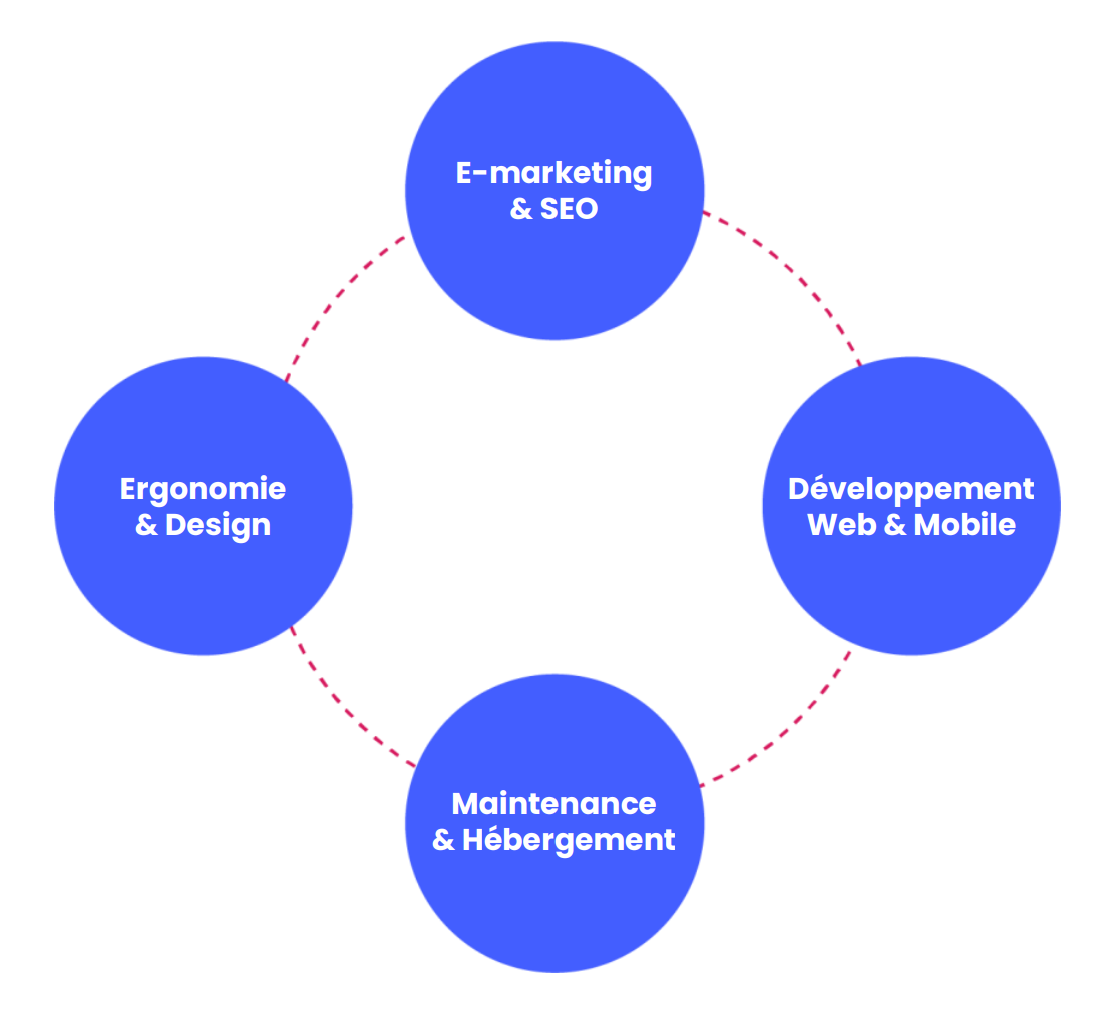
\includegraphics[width=12cm]{presentation/domaine.png}}
    \caption{différents domaines de mobelite}
\end{figure}

\subsection{\fontfamily{ptm}\selectfont\Large Problématique }
Le déploiement des systèmes de gestion de code source tells que Nexus, SonarQube ou le Monitoring sur un seul serveur local présente plusieurs problèmes qui affectent la performance de serveur et qui rendent l’exécution des diffèrentes applications ou l’ajout des nouvelles fonctionnalités plus difficile . Aussi, la maintenance de plusieurs applications en même temps sera compliquée et nécessite une planification minutieuse pour éviter l’interruption des processus d’autres applications. Les besoins d’entreprise changent au cours des temps et la capacité d'un seul serveur sera insuffisante pour rependre à la charge des données. Les mise à jour des applications peuvent impacter d'autres applications à cause de limites des ressources. En terme de sécurité, une attaque sur le serveur cause une perte des données très grande que sera difficile de récupérer en conséquence de l’utilisation d'un seul serveur.
C'est dans ce cadre que la société souhaite créer son propre solution .
\subsection{\fontfamily{ptm}\selectfont\Large Notion de base}
 Dans ce qui suit,nous présentons les notions de base que nous utiliserons pour réaliser le projet.
\subsubsection{\fontfamily{ptm}\selectfont\Large  Microservice}
    Avant l'apparition de l'architecture micro-service, les applications sont construites de manière monolithique, qui est considérée aujourd’hui comme méthode impertinente. L’utilisation de l'architecture monolithique, rend l’application très
    volumineuse avec des difficultés à enrichir les fonctions et le traitement des problèmes.
    Les microservices créent une application unique à partir de plusieurs petits services reliés de manière flexible.
    Ces services ont leur propre logique et leur propre base de données pour un usage spécifique. Chaque service peut être développé, mis à jour, déployé et mis à l’échelle sans affecter les autres services. Les mises à jour logicielles peuvent être plus fréquentes, ce qui améliore la fiabilité, la disponibilité et les performances(Voir figure 1.3). 

\begin{figure}[H]
    \begin{center}
    \fbox{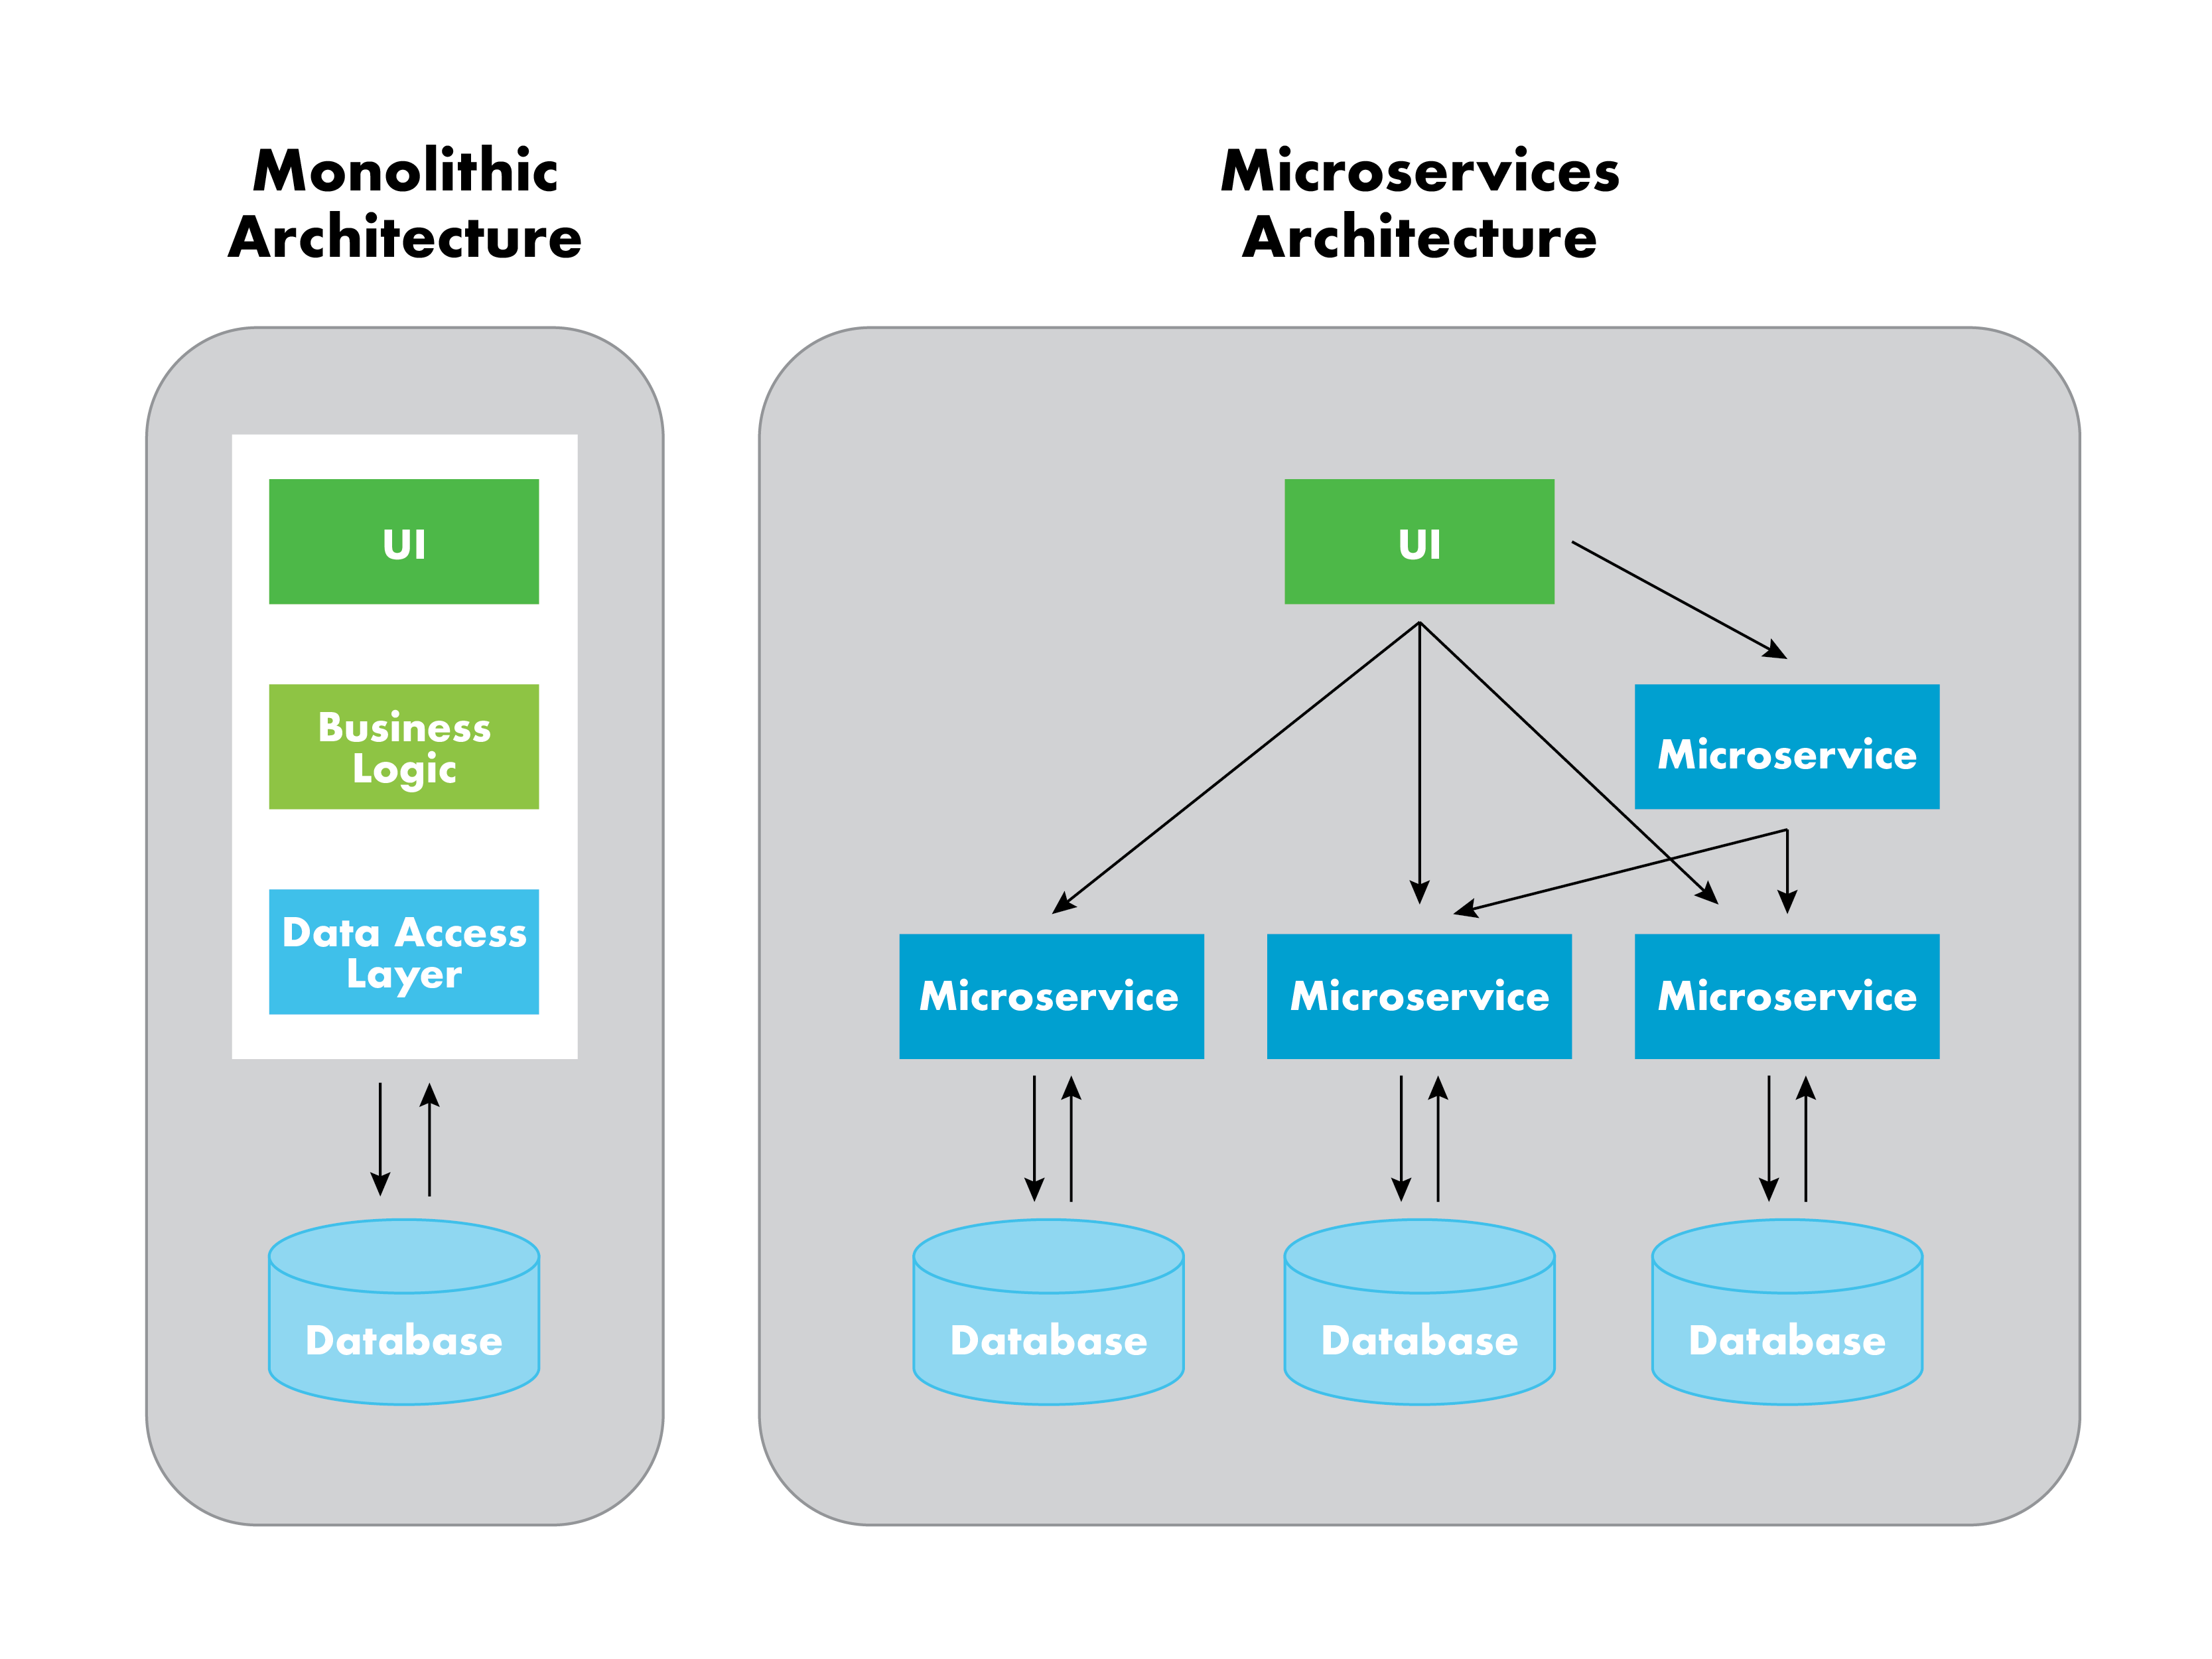
\includegraphics[height=11cm]{presentation/Microservice.png}}
    \end{center}
    \caption{Architecture monolithique vs Micro services}
\end{figure}
\subsubsection{\fontfamily{ptm}\selectfont\Large  DevOps}

    Combinant développement (Dev) et opérations (Ops), DevOps est l'union des personnes, des processus et des technologies destinés à fournir continuellement de la valeur aux clients.
    DevOps permet la coordination et la collaboration des rôles autrefois cloisonnés (développement, opérations informatiques, ingénierie qualité et sécurité) pour créer des produits plus performantes et plus fiables. En adoptant une culture DevOps ,ainsi que des pratiques et outils DevOps, les équipes peuvent mieux répondre aux besoins des clients, accroître la confiance suscitée par les applications qu'elles développent, et atteindre plus rapidement les objectifs de leur entreprise \cite{1} (voir figure 1.4).
    \begin{figure}[H]
    \begin{center}

    \fbox{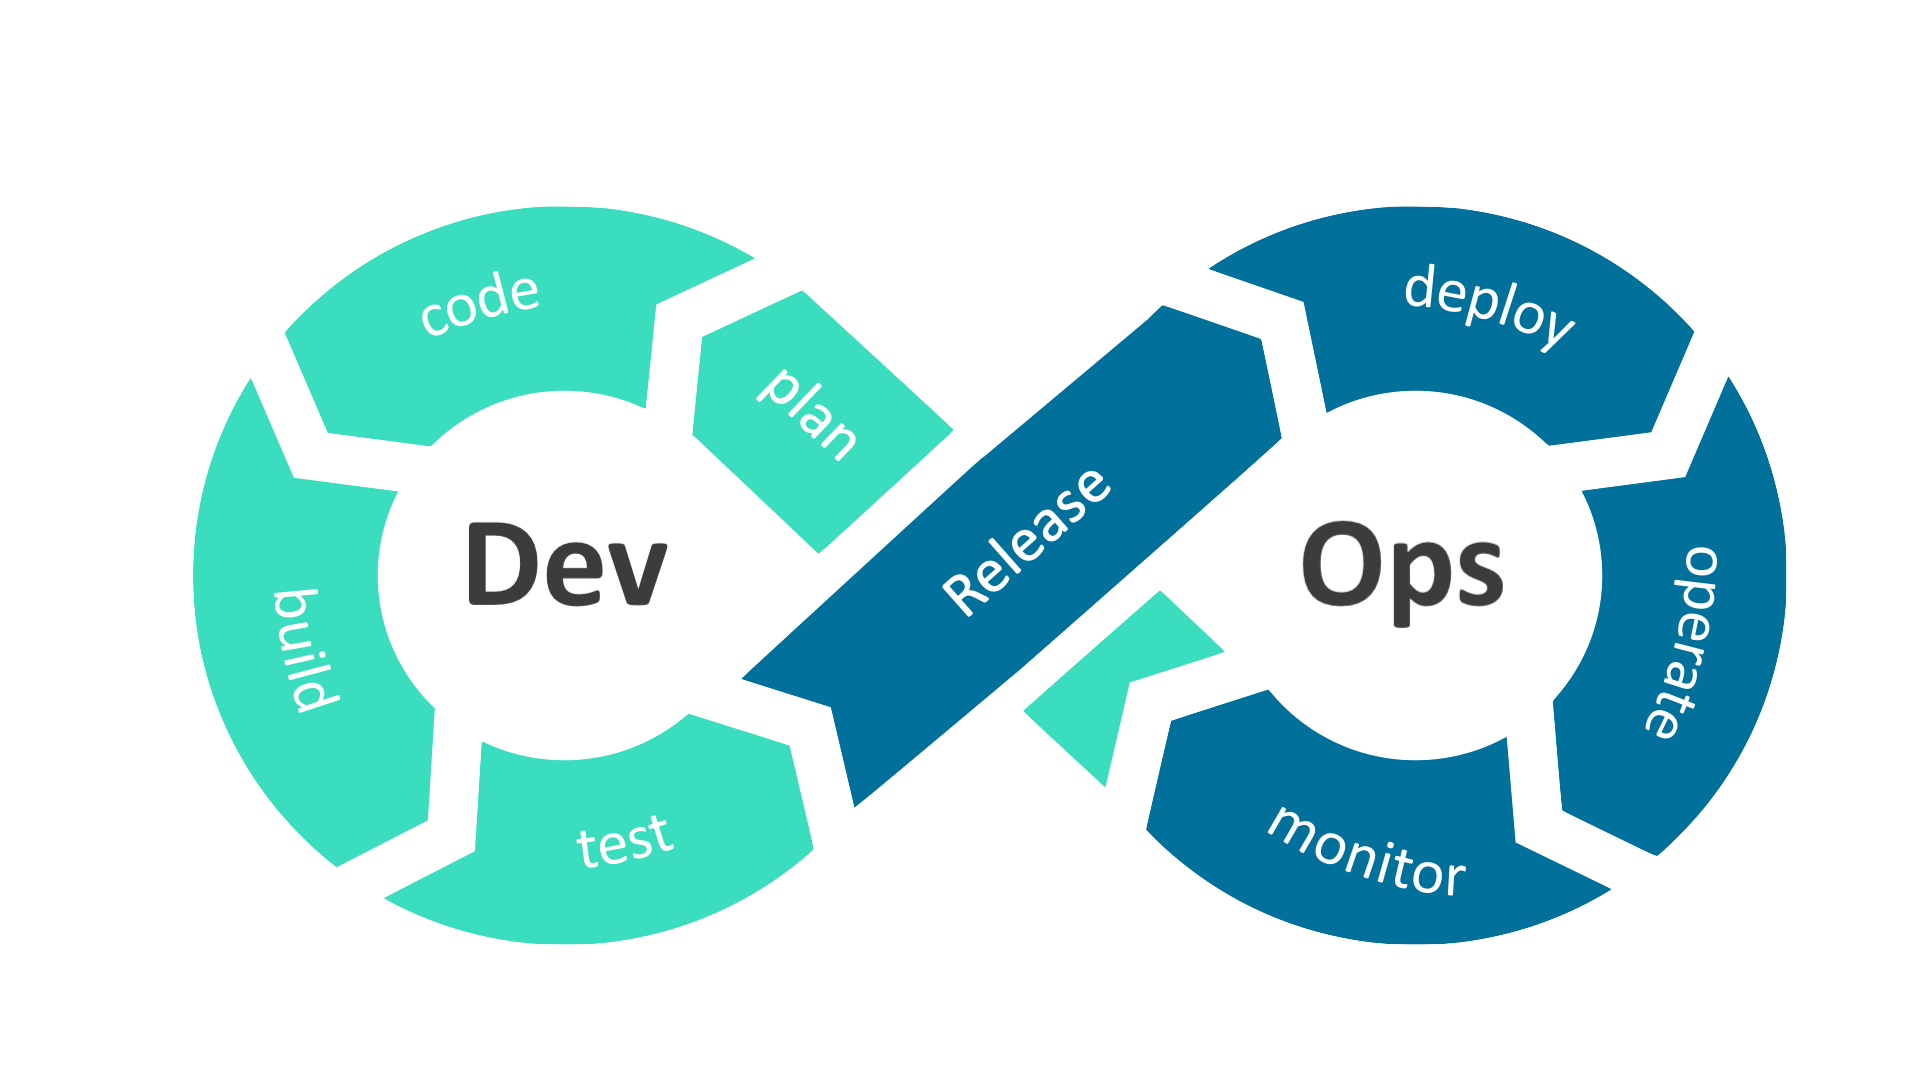
\includegraphics[height=8cm]{presentation/devops.png}}
    \end{center}

    \caption{Cycle de vie DevOps}
\end{figure}
%\textsf{}\\[0.1cm]
\subsubsection{\fontfamily{ptm}\selectfont\Large  Cloud}

 Le cloud n’est pas une entité physique, mais un vaste réseau de serveurs distants éparpillés tout autour de la planète, reliés entre eux, et destinés à fonctionner comme un écosystème unique. Ces serveurs sont conçus pour stocker et gérer des données, exécuter des applications, ou fournir du contenu ou des services (vidéos diffusées en continu, courrier web, logiciels bureautiques de productivité et autres réseaux sociaux). Au lieu d’accéder à des fichiers et données stockées sur un ordinateur local ou personnel, vous accédez à ces ressources en ligne à partir de n’importe quel appareil compatible avec Internet : les informations sont disponibles en tout lieu et tout le temps.\cite{2} 
\paragraph{\fontfamily{ptm}\selectfont\Large Modèles de services }
\texttt{}\\[0.2cm]
Il existe 3 modèles de services sur le cloud:\\[0.1cm]
\par \noindent \textbf{\Large -Software as a Service (SaaS): }Le Software as a Service, également connu sous le nom de SaaS, est un service basé sur le cloud où, au lieu de télécharger un logiciel que votre PC de bureau ou votre réseau professionnel peut exécuter et mettre à jour, vous accédez à une application via un navigateur internet. L'application logicielle peut être un logiciel de bureautique ou de communication unifiée parmi un large éventail d'autres applications professionnelles disponibles\cite{3} (voir figure 1.4).
%\begin{figure}[H]
%    \begin{center}
%\fbox{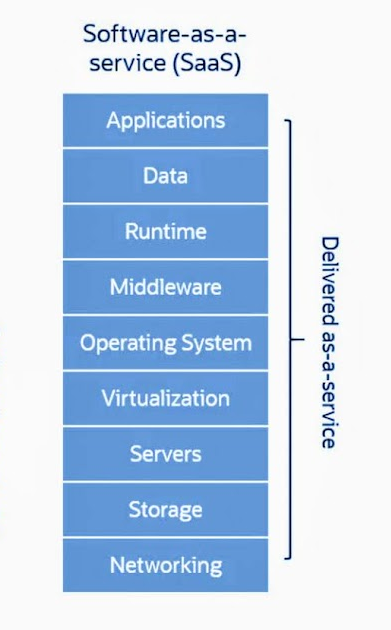
\includegraphics[height=8cm]{presentation/saas.png}}
%    \end{center}

%    \caption{ Architecture SaaS
%    }
%\end{figure}
\noindent \textbf{\Large -Platform as a Service (PaaS): } La Platform-as-a-service (PaaS) est un type d'offre de cloud computing dans lequel un fournisseur de services fournit une plateforme à ses clients, leur permettant de développer, d'exécuter et de gérer des applications commerciales sans avoir à construire et à maintenir l'infrastructure que ces processus de développement de logiciels requièrent généralement(Voir figure 1.4)\cite{4}.\\[0.1cm]
%\begin{figure}[H]
%    \begin{center}
%
%    \fbox{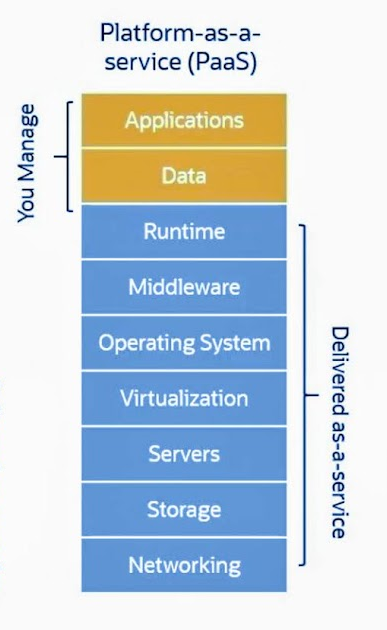
\includegraphics[height=8cm]{presentation/paas.png}}
%    \end{center}
%
%    \caption{ Architecture PaaS}
%\end{figure}
\noindent \textbf{\Large -Infrastructure as a Service (IaaS): }Infrastructure as a service (IaaS) est un type de service de cloud computing qui offre des ressources de calcul, de stockage et de mise en réseau essentielles à la demande, et sur une base de paiement à l’utilisation(Voir figure 1.4)\cite{5}.\\[0.1cm]
\begin{figure}[H]
    \begin{center}

    \fbox{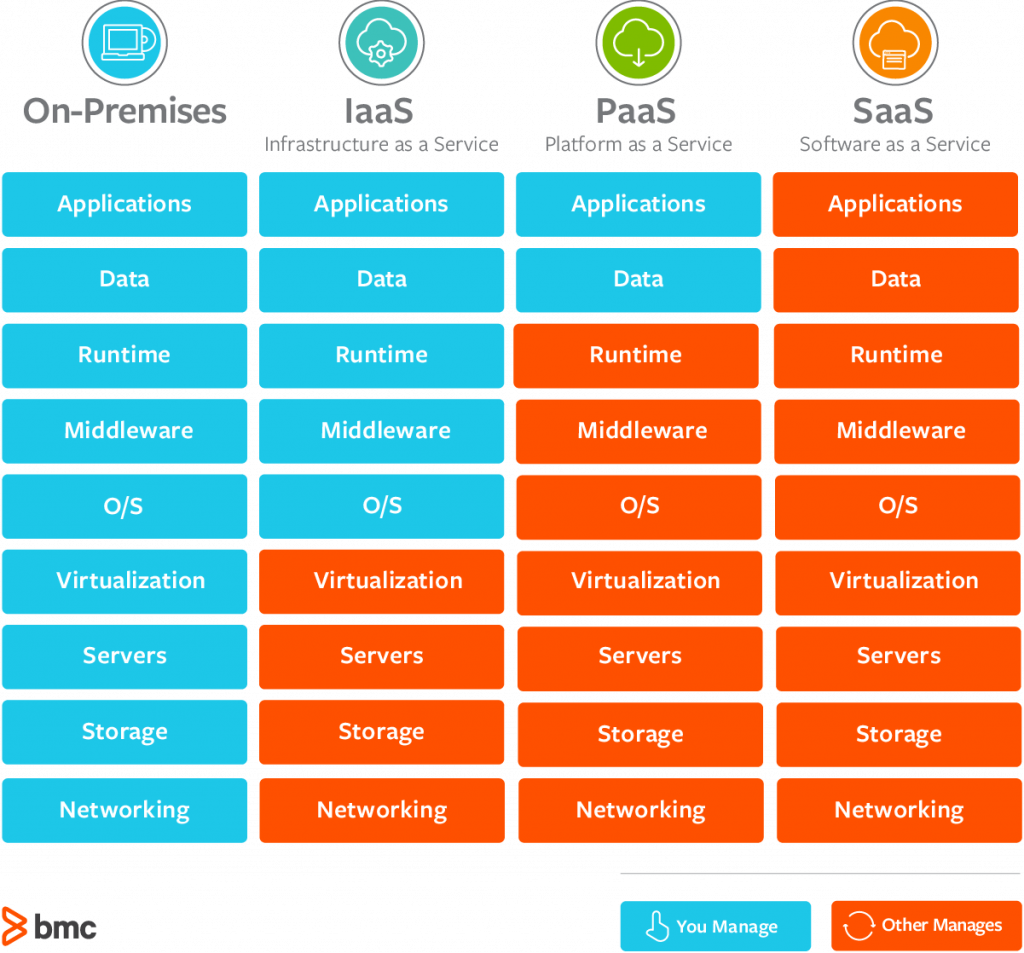
\includegraphics[height=10cm,width=13cm]{presentation/saas-vs-paas-vs-iaas-1024x953}}
    \end{center}

    \caption{ Différents architecture entre SaaS ,PaaS et IaaS}
\end{figure}
\paragraph{\fontfamily{ptm}\selectfont\Large Les modèles de déploiement }
\texttt{}\\[0.2cm]
Il existe 3 modèles de déploiement sur le cloud:

\par \noindent \textbf{\Large -Cloud Privé:  } Le cloud privé est un modèle informatique qui offre un environnement propriétaire dédié à une seule entité commerciale. Comme les autres types d'environnements du cloud computing, le cloud privé fournit des ressources informatiques étendues et virtualisées via des composants physiques stockés sur place ou dans le centre de données d'un fournisseur\cite{6}.\\[0.1cm]

\noindent \textbf{\Large -Cloud Public: } Le cloud public est un type de calcul dans lequel les ressources sont proposées par un fournisseur tiers via Internet, et sont partagées par les organisations et les individus qui souhaitent les utiliser ou les acheter \cite{7}.\\[0.1cm]

\noindent \textbf{\Large -Cloud Hybride :  } Un cloud hybride est un environnement informatique mixte dans lequel des applications s'exécutent à l'aide d'une combinaison de ressources de calcul, de stockage et de services dans différents environnements (clouds publics et clouds privés, y compris des centres de données sur site ou en périphérie)\cite{8}(voir figure 1.5).\\[0.1cm]

\begin{figure}[H]
    \begin{center}
    \fbox{
\includegraphics[height=7cm]{presentation/cloud.png}}
    \end{center}

    \caption{ Différents type du cloud}
\end{figure}

\subsection{\fontfamily{ptm}\selectfont\Large Méthodologie de développement }

 Avant de réaliser un projet informatique, il est essentiel de sélectionner une démarche de travail et une procédure de suivi pour obtenir un logiciel stable. Il s'agit d'un cadre permettant de structurer, de planifier et de contrôler le développement d'une application.\\
Pour la réalisation de notre projet nous avons opté pour la méthodologie agile SCRUM car elle
améliorer la flexibilité de projet et réduit le temps de livraison de produits complet au client.En
effet , la plupart des projets réalisés dans l’entreprise appliquent cette méthodologie.
 \\[0.2cm]


%\begin{figure}[H]
%    \begin{center}
        %taille de l'image en largeur
        %remplacer "width" par "height" pour régler la hauteur
%    \fbox{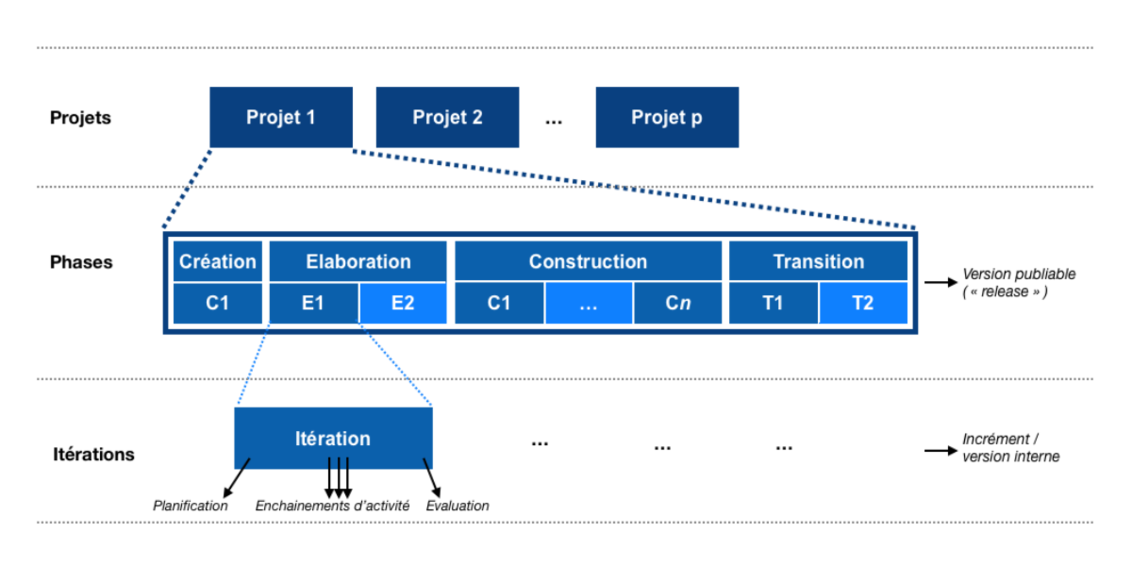
\includegraphics[height=6cm]{2 tracks unified process}}
%    \end{center}
    %légende de l'image
%    \caption{Cycle de vie de projet avec le processus unifié }
%\end{figure}
%\texttt{}\\[0.2cm]
\subsubsection{\fontfamily{ptm}\selectfont\Large Méthode agile }

Agile est une méthode de gestion de projet conçue pour distribuer en continu les logiciels opérationnels en fonction d'itérations rapides. Il permet aux équipes de développer progressivement un produit de qualité et d'adapter leur processus en fonction des besoins du projet.


\paragraph{\fontfamily{ptm}\selectfont\Large  Présentation de la méthodologie Scrum}
\texttt{}\\[0.2cm]

Scrum est une méthodologie agile pour l'élaboration, la réalisation et le soutien de projets complexes. Elle est basée sur la division du produit sur différentes itération sprints.
Scrum est plus utile lorsque les exigenes sont variables et peuvent changer beaucoup de fois au cours du cycle de vie, ce qui donne donc la capacité d'avoir un projet flexible capable de traiter les changements fréquents.
\paragraph{\fontfamily{ptm}\selectfont\Large    Acteurs de la méthode agile Scrum}
\texttt{}\\[0.2cm]

Méthode agile Scrum se compose par 3  acteurs ce suit:
\par \noindent \textbf{\Large -Scrum Master: } Il s'agit de la personne chargée d'orienter l'équipe de travail vers la bonne voie, d'assurer la bonne pratique des règles de la méthode Scrum et d'organiser son équipe. \\[0.1cm]

\noindent \textbf{\Large -Product Owner: } il représente les clients et assure que leurs besoins et visions soient réalisés dans le projet. Il travaille généralement en collaboration directe avec l’équipe de développement. \\[0.1cm]

\noindent \textbf{\Large -Equipe de développement: }sont les personnes responsables de la transformation des besoins du client. Ces besoins sont définis par le Product Owner à travers des fonctions utilisables. L'équipe est composée d'au moins 3 personnes jouant les rôles de développeur ou de concepteur.\\[0.1cm]
\paragraph{\fontfamily{ptm}\selectfont\Large Évènements de la méthode agile Scrum }
\texttt{}\\[0.2cm]
 Scrum définit cinq types d'évènements :\\[0.1cm]%????????????????
\par \noindent \textbf{\Large -Le sprint: }Chaque sprint est de durée maximale de 4 semaines pendant laquelle une version de produit est réalisée. Une fois un sprint terminé un nouveau a déjà commencé avec une liste de fonctionnalités et un objéctif à réaliser. \\[0.1cm]

\noindent \textbf{\Large -Planification d’un sprint: }À chaque début de sprint, cette réunion est conçue pour déterminer les tâches à réaliser pendant le sprint. L’organisation de ces tâches est effectuée par l’équipe de développement et le Product Owner. \\[0.1cm]

\noindent \textbf{\Large -Mêlée quotidienne: } C'est une réunion d'une durée de 15 minutes faite par l’équipe chaque jour pour définir l’objectif de la journée et identifier les obstacles s’il y en a quelques-uns.\\[0.1cm]

\noindent \textbf{\Large -Revue de sprint: }  Représente le travail réalisé par l’équipe au cours du sprint et le comparer avec le produit attendu.\\[0.1cm]

\noindent \textbf{\Large -Rétrospective de sprint: } Le but de cet événement est de déterminer les problèmes intervenus dans la période du sprint, l’efficacité des outils et déterminer ce qui peut être amélioré.

\paragraph{ \fontfamily{ptm}\selectfont\Large Les artefacts}
\texttt{}\\[0.2cm]
\noindent \textbf{\Large -Product Backlog: }
  Il s’agit d’une liste des besoins et exigences à recueillir pour créer le produit désiré, ce document est la responsabilité de Product Owner(voir figure 1.6).\\[0.1cm]

\noindent \textbf{\Large -Sprint Backlog: } C’est l’ensemble des données permettant la réalisation des objectifs du sprint. Ce document est mis à jour par l’équipe de développement régulièrement.

\begin{figure}[H]
    \begin{center}
        %taille de l'image en largeur
        %remplacer "width" par "height" pour régler la hauteur
    \fbox{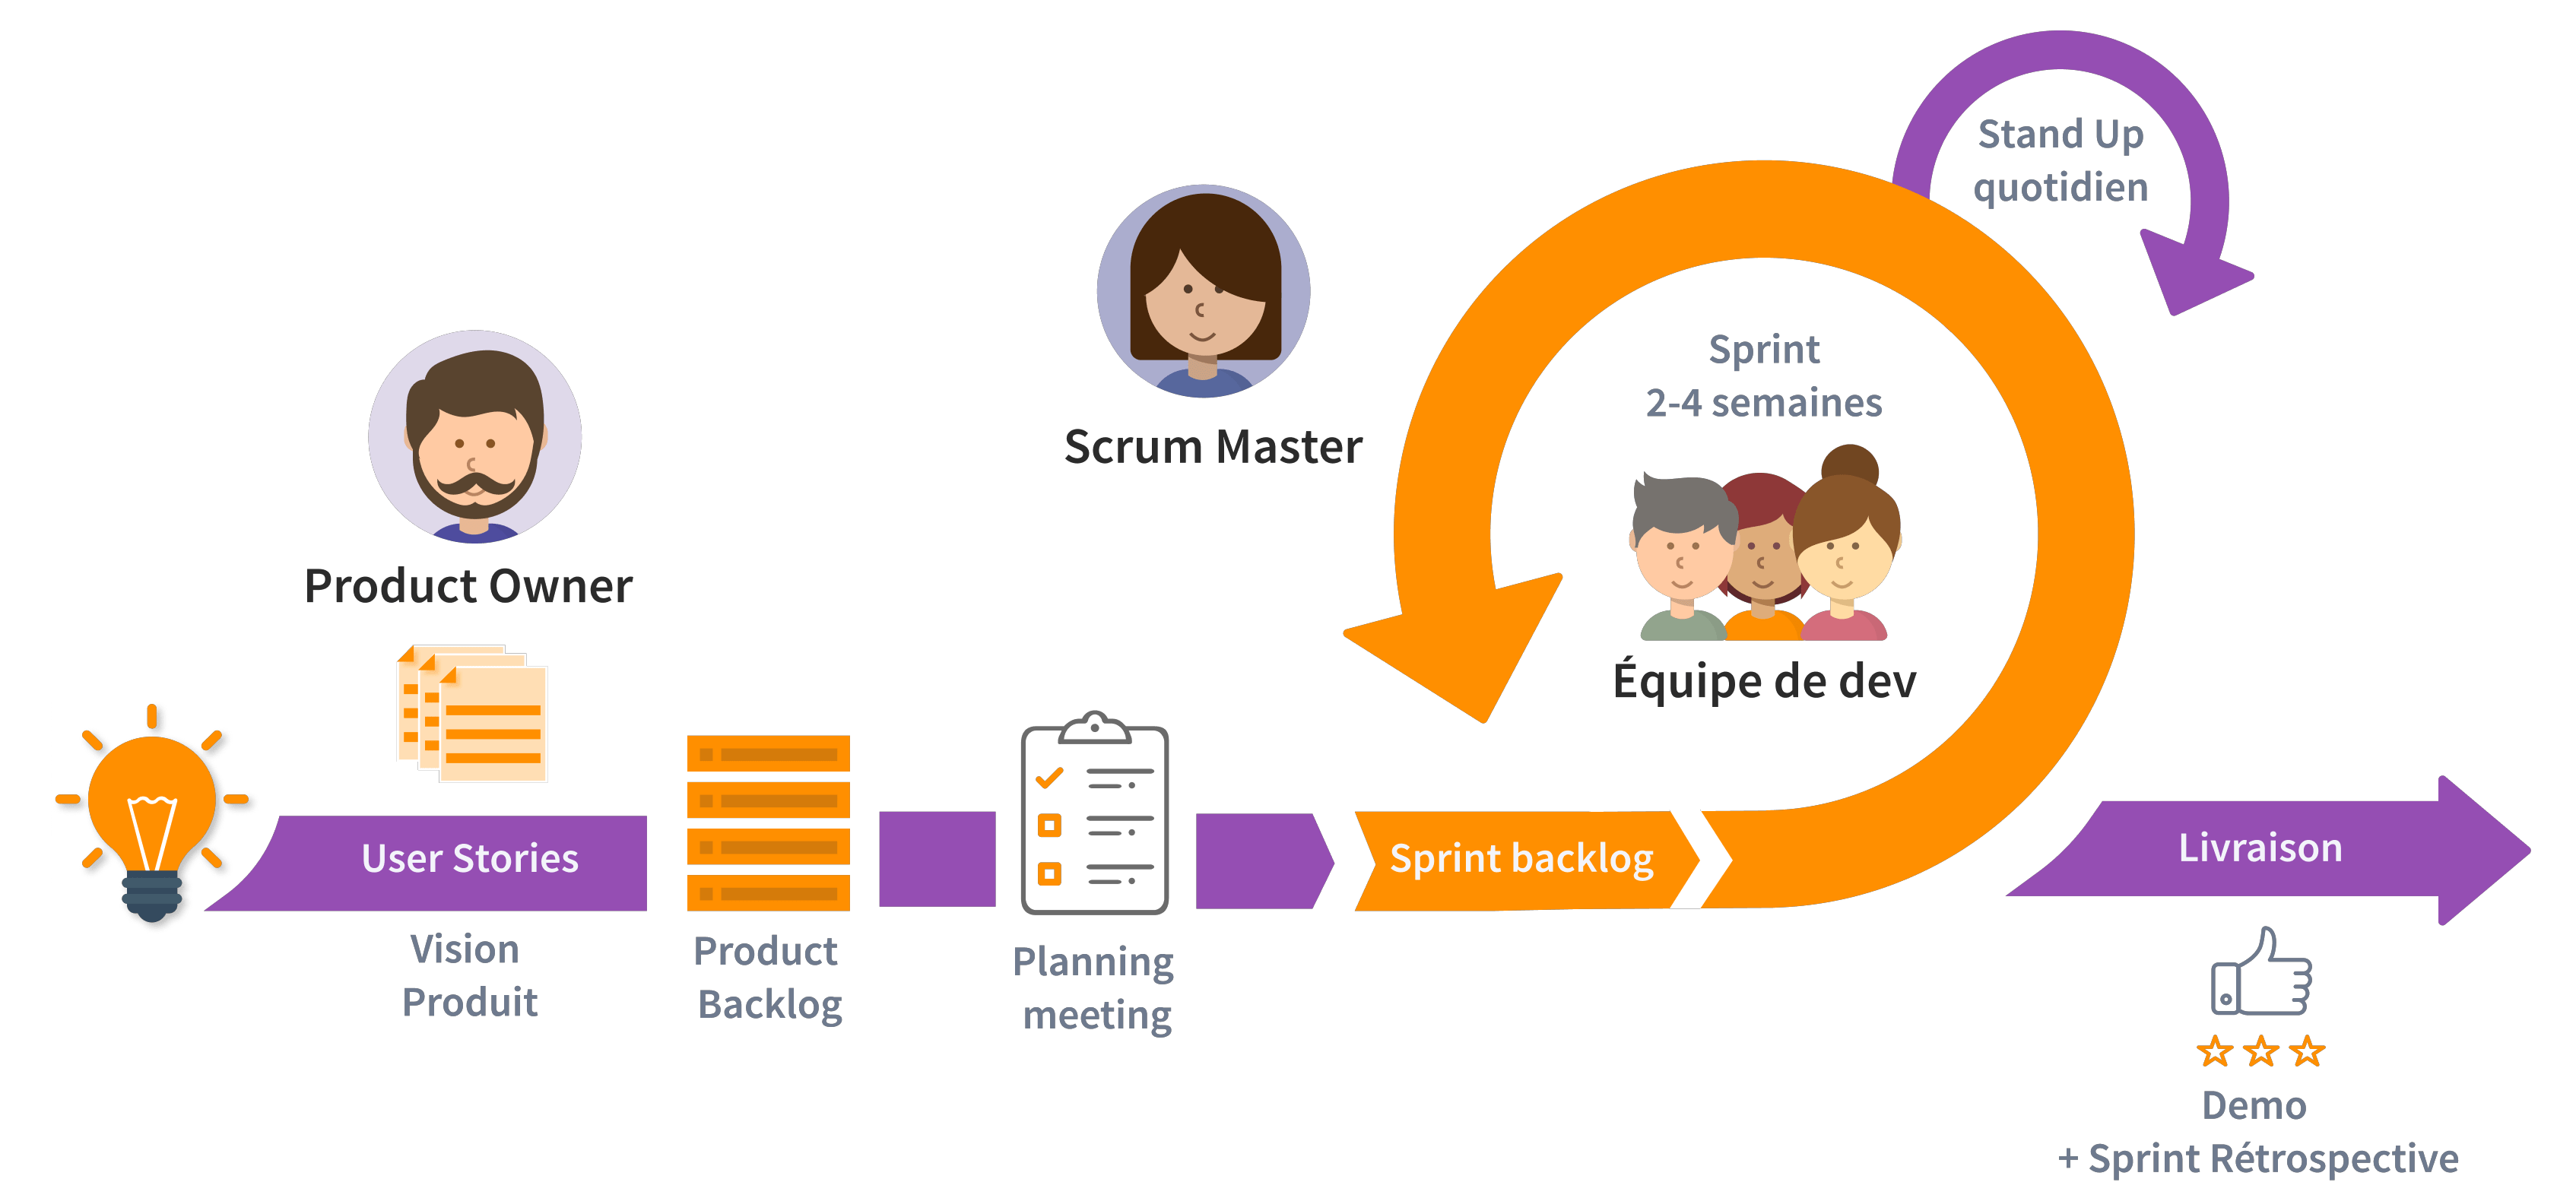
\includegraphics[height=7cm]{agile-Scrum-sprint-workflow-schema-FR.png}}
    \end{center}
    %légende de l'image
    \caption{Processus de méthode Scrum}
\end{figure}


\subsection{\fontfamily{ptm}\selectfont\Large Planification des sprints}
 
Pour une meilleure optimisation  du développement du projet nous avons divisé le travail en des Sprints présentés dans un diagramme de Gantt qui décrit l’état d’avancement dans le temps des différentes activités (voir figure 1.7):

\begin{figure}[H]
    \begin{center}
        %taille de l'image en largeur
        %remplacer "width" par "height" pour régler la hauteur
    \fbox{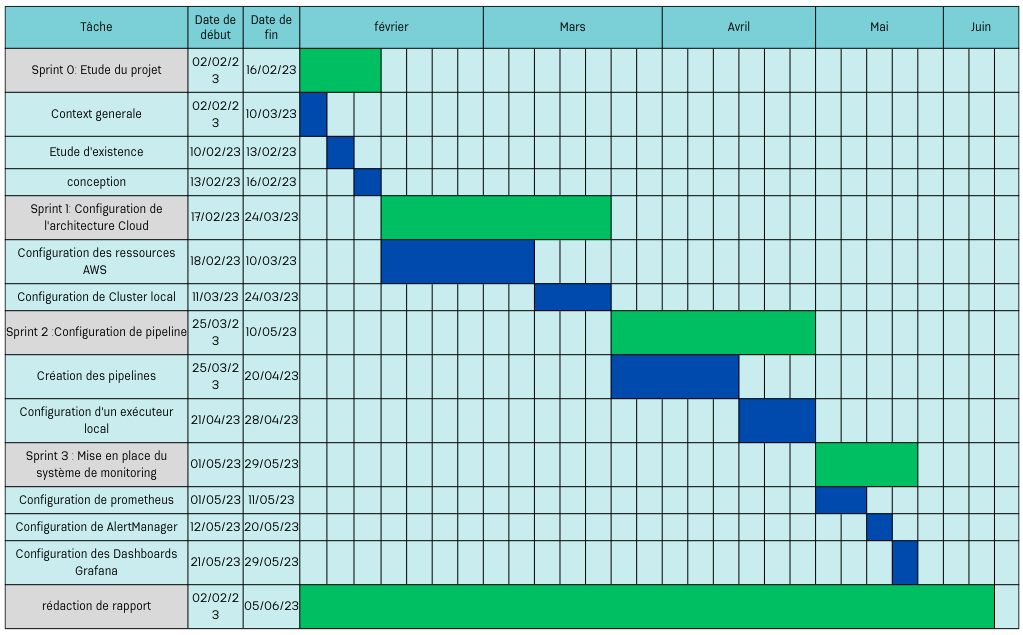
\includegraphics[height=11cm]{presentation/Gantt.png}}
    \end{center}
    %légende de l'image
    \caption{Diagramme de Gantt}
\end{figure}

\subsection{\fontfamily{ptm}\selectfont\Large    Conclusion}

 Dans ce chapitre nous avons présenté la société d’accueil, la problématique et la méthodologie de développement.
    Dans le prochain chapitre, nous allons faire une étude de l’existant à travers une comparaison des solutions sur le marché afin de proposer notre solution.

\chapter{ Etude de l'existant}
\newpage
\textbf{\huge Introduction} \\[1cm]
\textsf{\fontfamily{qtm}\selectfont\scalefont{1.3}
L’objectif de ce deuxième chapitre est la présentation des solutions existantes sur le marché avec une étude comparative et présentation de la solution proposée.
}\\[0.1cm]


\section{\LARGE Les solutions existantes}
\texttt{}\\[0.1cm]
\textsf{\fontfamily{qtm}\selectfont\scalefont{1.3} L'entreprises a des besoins sur mesure. C'est pourqouien revue les solutions similaires à notre solution. Nous allons étudier les points forts ainsi que les points faibles de ces solutions afin de montrer pourquoi nous devrions developper notre propre solution. Voici une présentation de certaines solutions existantes :}
\subsection{\LARGE Azure Devops}
\texttt{}\\[0.1cm]
\textsf{\fontfamily{qtm}\selectfont\scalefont{1.3}Azure DevOps prend en charge une culture collaborative et un ensemble de processus qui rassemblent les développeurs, les responsables de projets et les contributeurs pour développer des logiciels. Elle permet aux organisations de créer et d’améliorer les produits à un rythme plus rapide que possible avec les approches traditionnelles de développement de logiciels.Azure DevOps Services vous donne également accès aux serveurs de génération et de déploiement cloud et aux insights sur les applications. Démarrez gratuitement et créez une organisation. Ensuite, chargez votre code pour partager ou contrôler le code source. Commencez à suivre votre travail à l’aide de Scrum, Kanban ou d’une combinaison de méthodes.(Voir figure 2.1)\cite{9}}
\textsf{\fontfamily{qtm}\selectfont\scalefont{1.3}Elle a des avantages mais aussi des inconvenients:}\\[0.1cm]
\par \noindent \textbf{\Large -Avantage:}
\textsf{\fontfamily{qtm}\selectfont\scalefont{1.3}Azure offre une haute disponibilité,sécurité solide et offre de bonnes options d’évolutivité.}\\[0.1cm]
\par \noindent \textbf{\Large -Inconvenient:}
\textsf{\fontfamily{qtm}\selectfont\scalefont{1.3}oblige à mettre tous vos oeufs dans le même panier et la facilité d’accès peut être problématique pour certaines entreprises.}\\[0.1cm]
\par \noindent \textbf{\Large -Collaboration tools:}
\textsf{\fontfamily{qtm}\selectfont\scalefont{1.3}}
\begin{figure}[H]
    \begin{center}
    
        \fbox{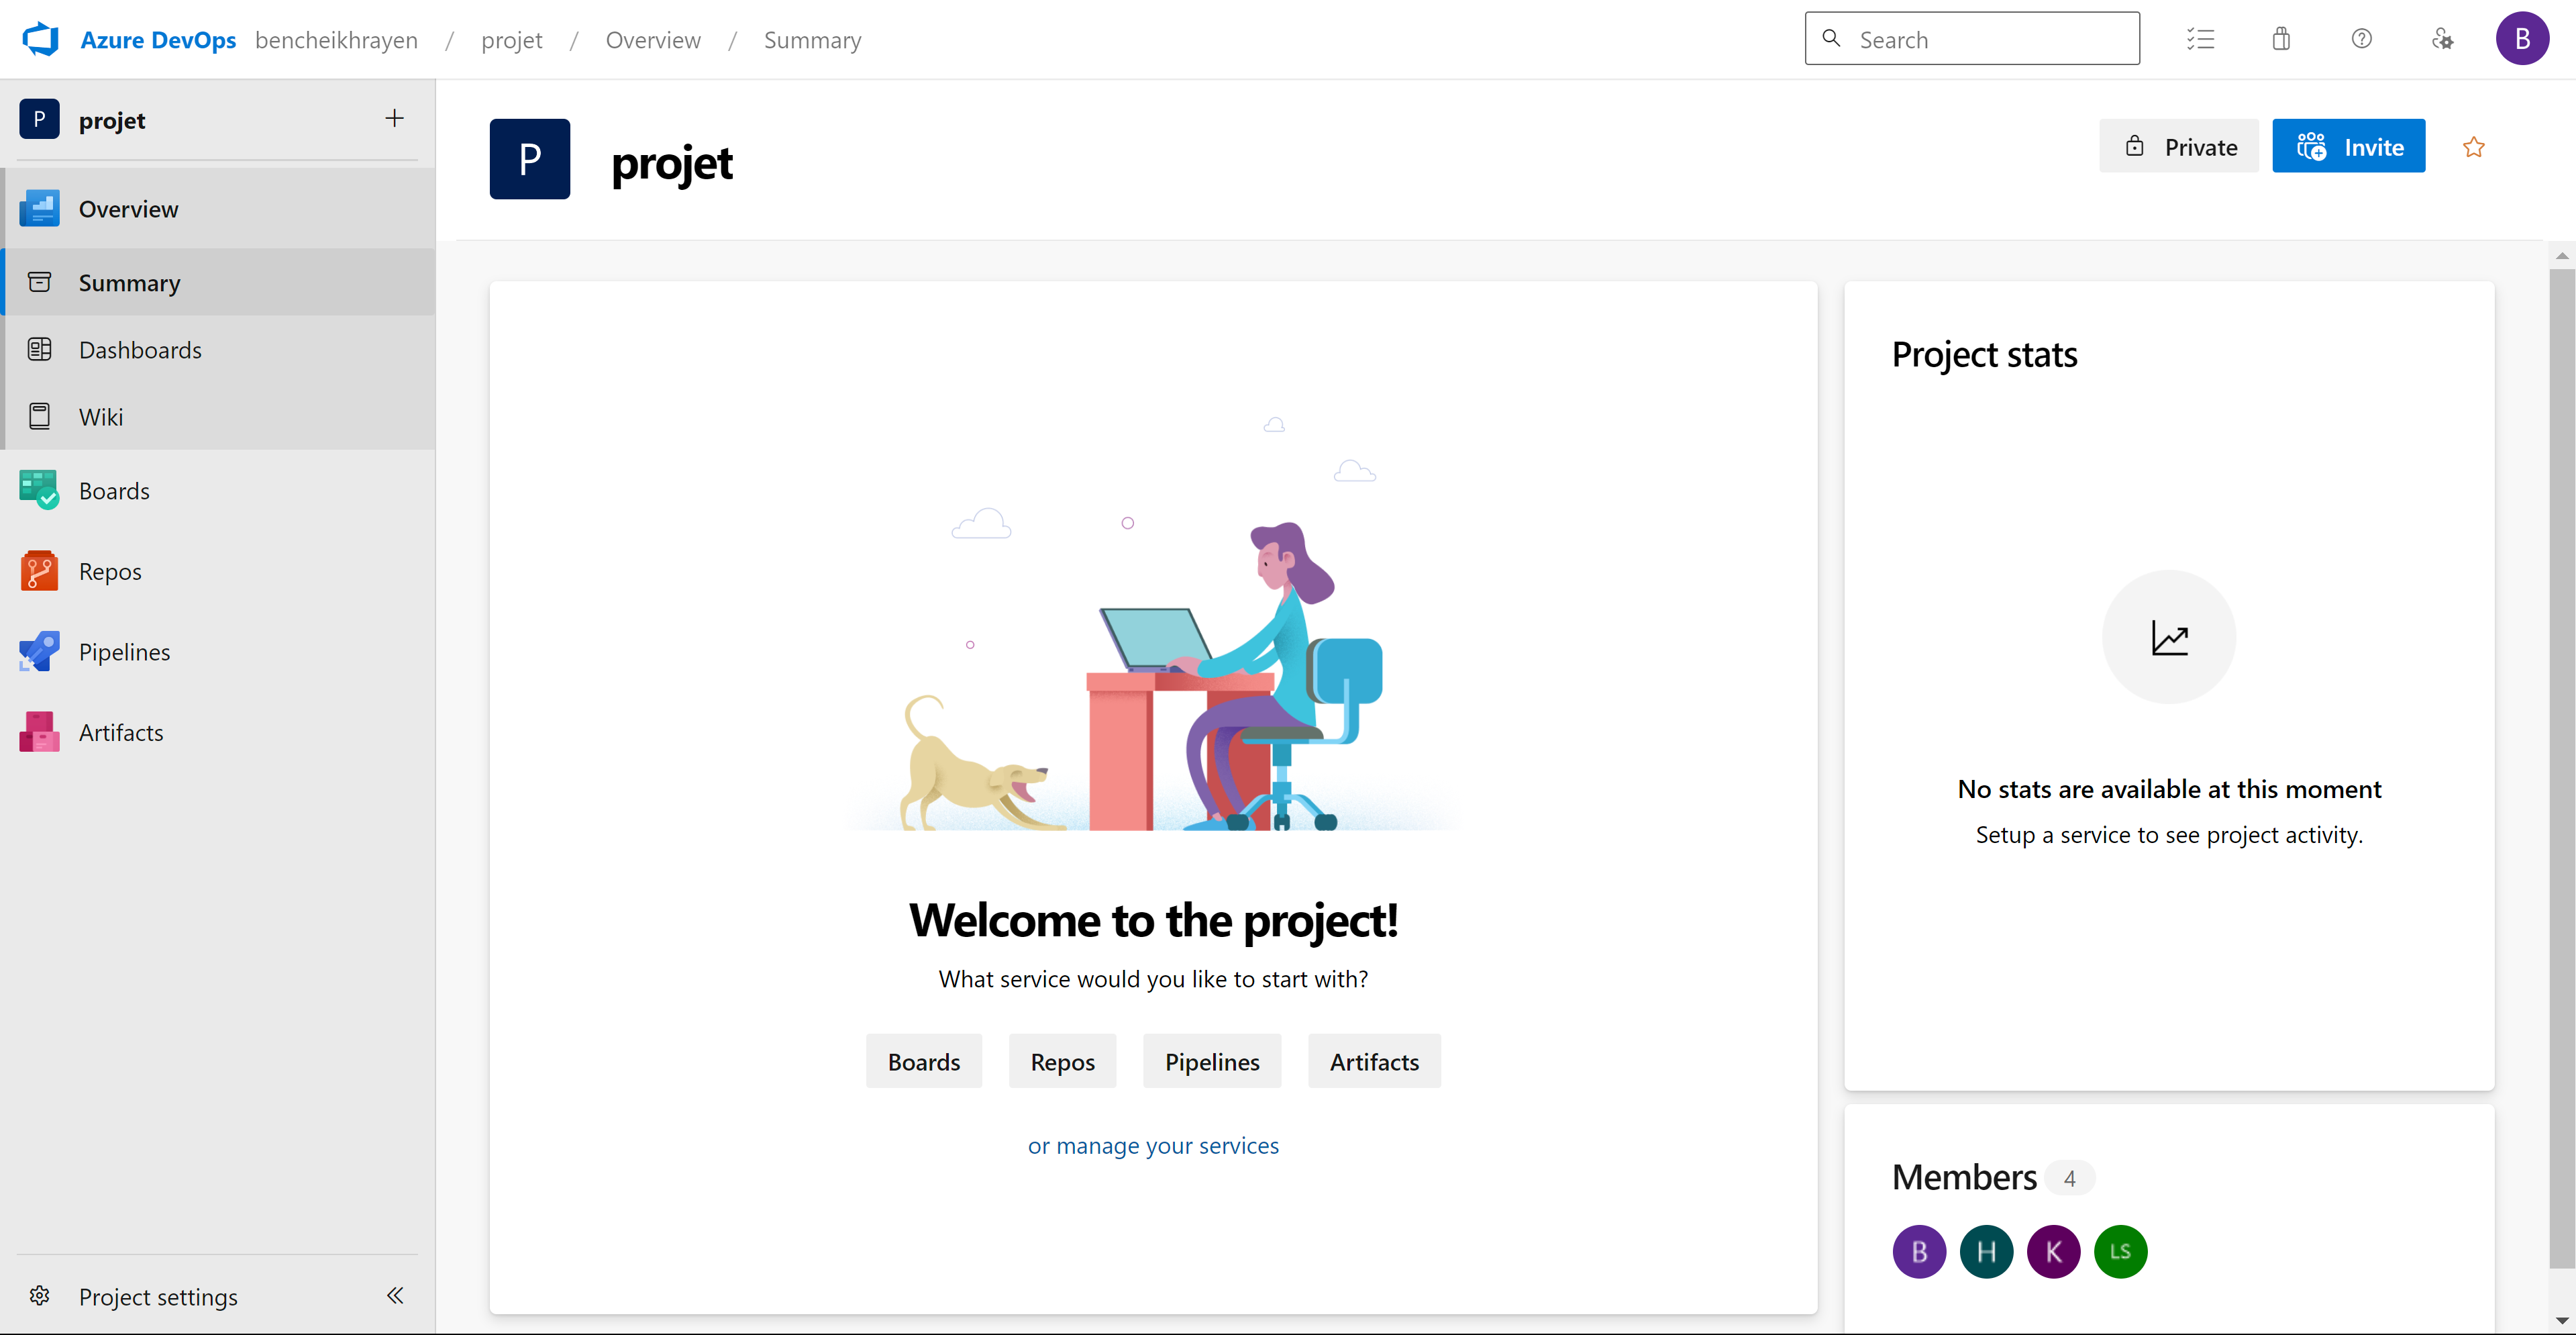
\includegraphics[width=12cm]{azure.png}}

    \end{center}
    
    \caption{Azure DevOps}
\end{figure}

\subsection{\LARGE Amazon Web Service DevOps}
\texttt{}\\[0.1cm]
\textsf{\fontfamily{qtm}\selectfont\scalefont{1.3} AWS fournit un ensemble de services flexibles, conçus pour permettre aux entreprises de créer et livrer des produits avec plus de rapidité et de fiabilité à l'aide d'AWS et des pratiques de DevOps. Ces services simplifient la mise en service et la gestion de l'infrastructure, le déploiement de code d'application, l'automatisation des processus de publication de logiciel et le suivi des performances de l'application et de l'infrastructure(Voir figure 2.2).Cependant, comme toute autre technologie, AWS présente des avantages et des inconvénients: \cite{10}}\\[0.1cm]
\par \noindent \textbf{\Large -Avantage:}
\textsf{\fontfamily{qtm}\selectfont\scalefont{1.3}Aws offre une grande évolutivité pour les entreprises peuvent facilement augmenter ou réduire leurs ressources en fonction de leurs besoins .Aussi , il présente un niveau de fiabilité élevé et il fournit aux entreprises une gamme de services, notamment le stockage, la gestion de bases de données, la puissance de calcul et l’analyse}\\[0.1cm]
\par \noindent \textbf{\Large -Inconvenient:}
\textsf{\fontfamily{qtm}\selectfont\scalefont{1.3}AWS est complexe à mettre en place et à gérer ses ressources. Aussi, les entreprises doivent prendre des mesures pour garantir la protection de leurs données.}
\begin{figure}[H]
  \begin{center}
  
      \fbox{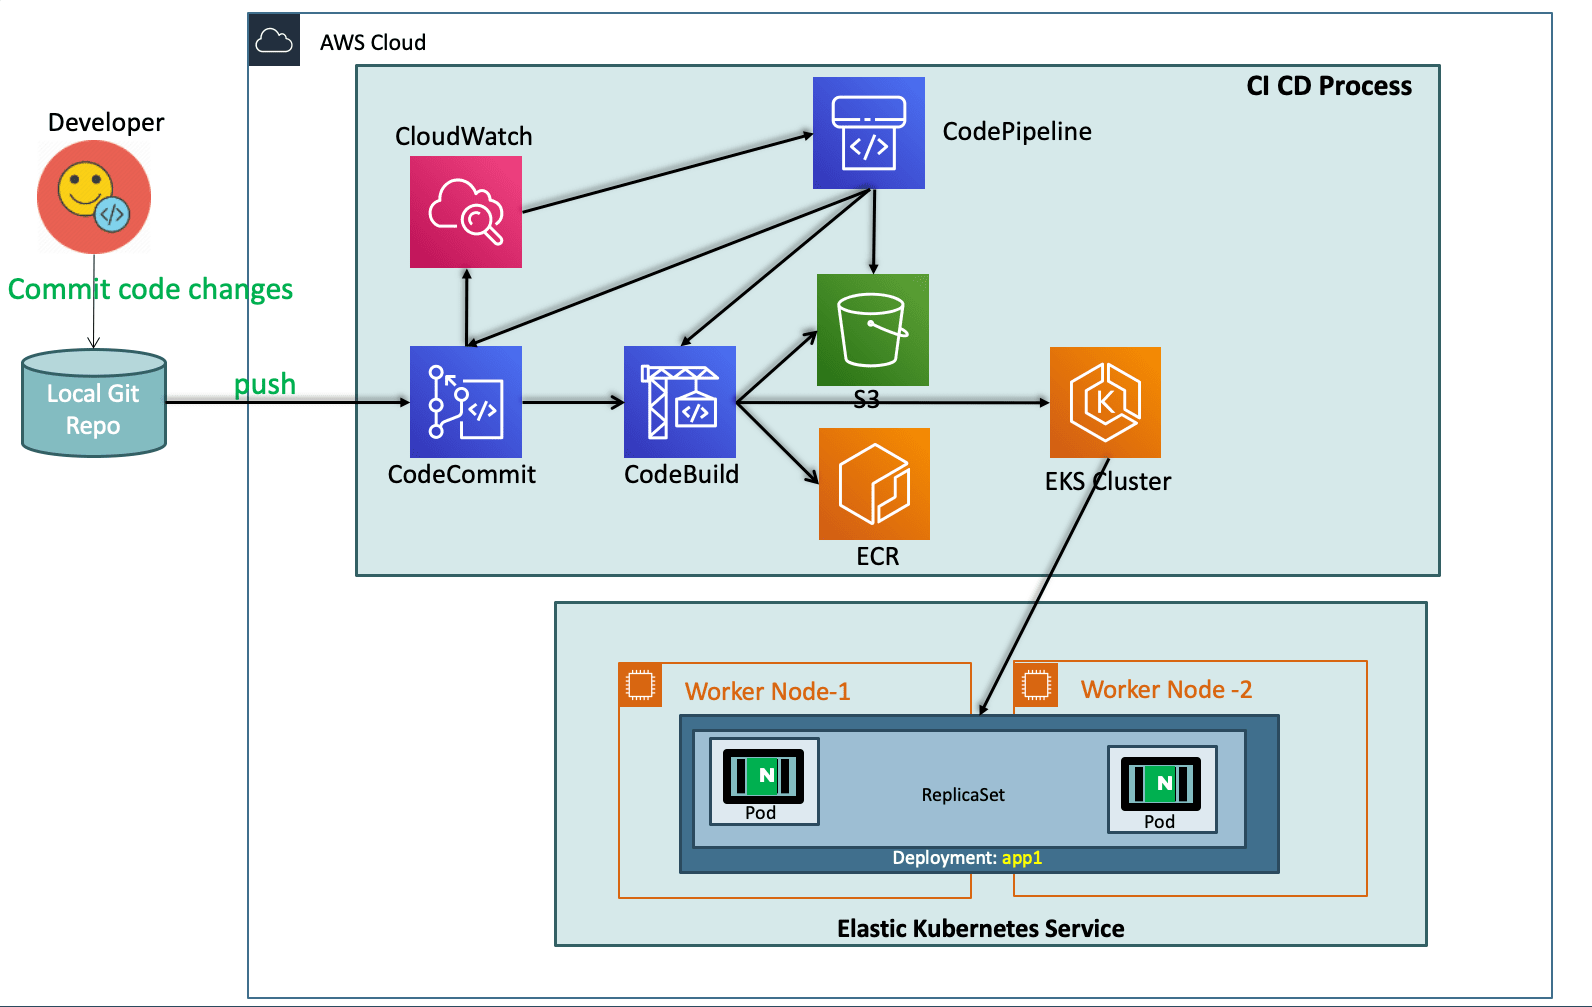
\includegraphics[width=12cm]{aws.png}}

  \end{center}
  
  \caption{Amazon Web Services}
\end{figure}
\subsection{\LARGE Google Cloud Platform DevOps }
\texttt{}\\[0.1cm]
\textsf{\fontfamily{qtm}\selectfont\scalefont{1.3}
Google propose de nombreux services et fonctionnalités visant à aider les ingénieurs DevOps à disposer de tout ce dont ils ont besoin pour respecter les normes de qualité et de sécurité les plus élevées tout en automatisant la majorité du processus.De plus, vous travaillez avec des outils GCP DevOps efficaces qui non seulement augmentent la qualité des applications, mais améliorent également la vitesse du cycle de développement. Ces outils DevOps s’adressent directement aux ingénieurs logiciels car ils permettent une configuration rapide et simple, avec une interface intuitive qui facilite l’utilisation efficace des outils et méthodologies de livraison continue et de déploiement continu (intégration continue/ déploiement continu(CI/CD))(Voir figure 2.3).Ainsi GCP a des points forts et des points faibes:\cite{11}}
\par \noindent \textbf{\Large -Points forts :}
\textsf{\fontfamily{qtm}\selectfont\scalefont{1.3} GCP offre également des services de développement et d’intégration d’applications aussi une bonne Sécurité .}\\[0.1cm]
\par \noindent \textbf{\Large -Points faibles:}
\textsf{\fontfamily{qtm}\selectfont\scalefont{1.3}  certaines intégrations peuvent être plus étroites avec les services et les outils de Google par rapport aux solutions tierces.Aussi ,la  configuration initiale de GCP est complexe en raison de la vaste gamme de services et d'options disponibles.}\\[0.1cm]
\begin{figure}[H]
  \begin{center}
  
      \fbox{
\includegraphics[width=12cm]{gcp.png}}

  \end{center}
  
  \caption{Google Cloud Platform}
\end{figure}
\section{\LARGE Critique des solutions existantes}
\texttt{}\\[0.1cm]
\textsf{\fontfamily{qtm}\selectfont\scalefont{1.3}
Nous allons comparer les solutions présentées ci-dessus selon plusieur qu'on definire par rapport aux besoins de l'entreprise.}\\[0.1cm]
\begin{tabular}{|c|c|c|c|}
\hline
 & Azure Devops & \ Amazon Web Service DevOps & Google Cloud Platform DevOps\\
\hline
C 1 & \textbf{X} &  & \\
\hline
C 2 & & \textbf{X} & \textbf{X} \\
\hline
C 3 & & \textbf{X} &  \\
\hline
C 4 & & & \\
\hline
\end{tabular}
\texttt{}\\[0.1cm]
\textsf{\fontfamily{qtm}\selectfont\scalefont{1.3} En se basant sur le tabeau comparatif ci-dessous,on constate que AWS est plus fiable pour notre sujet mais il n'est pas compatible avec notre projet.}\\[0.1cm]
\par \noindent \textbf{\Large C1 - La confidentialité des données d'application : }\textsf{\fontfamily{qtm}\selectfont\scalefont{1.3} La solution doit privilégier la confidentialité des données puisque certains clients préfèrent leur application exécutée sur le serveur local de la société.} \\[0.1cm]

\noindent \textbf{\Large C2 - Intégration de solutions open source : }\textsf{\fontfamily{qtm}\selectfont\scalefont{1.3} Amazon cloud, azure cloud ou toute autre solution cloud doit intégrer certaines software open source comme services à utiliser dans votre architecture cloud.Bien que les logiciels libres puissent être hautement personnalisables, le niveau de personnalisation fourni par un fournisseur de services peut être restreint. }\\[0.1cm]
\noindent \textbf{\Large C3 - Coût de projet : }\textsf{\fontfamily{qtm}\selectfont\scalefont{1.3}  L'utilisation d'Amazon Cloud ainsi tout autre fournisseur pour  déployer une application dans le Cloud semble peu coûteux au début, mais après que la charge de travail augmente, les coûts aussi augmentent . Il s'agit de trouver une solution qui profite du cloud et des avantages du logiciel libre.}\\[0.1cm]
\noindent \textbf{\Large C4 - Problèmes de compatibilité : }\textsf{\fontfamily{qtm}\selectfont\scalefont{1.3} La personnalisation peut présenter des problèmes de compatibilité, surtout si la personnalisation interagit avec d'autres services ou composants au cours du déploiement. Cela peut entraîner des temps d’arrêt ou d’autres problèmes de performance.}\\[0.5cm]
% \begin{flushleft} 
%   \textsf{\fontfamily{qtm}\selectfont\scalefont{1.8}\hyphenchar\font=-1 -- Voici un tableau récapitulatif de notre analyse de l'existant...\\
%   Légende : \\
% X : la soulution ne conforme pas a la demande de Sujet.\\
% \checkmark : la soulution conforme a la demande de Sujet.\\}
% \end{flushleft}
\textsf{\fontfamily{qtm}\selectfont\scalefont{1.5} --Notons que cette évaluation ne concerne que notre situation, dans d'autres cas les solutions existantes peuvent être utile.  }

%tableau centré à taille variable qui s'ajuste automatiquement suivant la longueur du contenu

% \begin{center}
% \begin{table}[H]  
%   \centering
% \begin{tabular}{|l|l|l|l|l|}
%   \hline
%   Critère/Solution &  GCP DevOps & AWS DevOps & Azure Devops\\
%   \hline
%   La confidentialité des données d'application & & &  \\
%   Intégration de solutions open source &  &  & \\
%   Coût de projet &  &  & \\
%   Problèmes de compatibilité& &  &  \\
%   \hline
% \end{tabular}
% \caption{Tableau comparatif des solutions existantes}
% \end{table}
% \end{center}
\section{\LARGE Solution proposée}
\texttt{}\\[0.1cm]
\textsf{\fontfamily{qtm}\selectfont\scalefont{1.3} Pour rectifier les problèmes auxquels l’équipe devops fait face chaque jour et afin de  préparer un environnement de développement flexible, Mobelite nous a proposé de mettre en place une solution Hybride cloud qui bénéficie à la fois  de certain services de cloud avec un accès privé aux données. En effet, le projet consiste à implémenter la conteneurisation qui nous offrira une virtualisation des ressources de manière légère, flexible et puissante. Le déploiement d’un kubernetes cluster qui est un système de gestion de conteneurs qu'on va utiliser pour optimiser le déploiement des applications avec l’utilisation d’autres produits comme Ansible pour l’optimisation de cette infrastructure. La solution a des objectifs importants pour l’entreprise comme la réduction des coûts de développement et d'exploitation. Le Cycle de développement sera plus court grâce à l'automatisation et le déploiement rapide des nouveaux environnements.Aussi, la solution garantira la supervision totale et continue de la plateforme, et la haute disponibilité du système.}\\[0.1cm]
\section{\LARGE    Conclusion}
\texttt{}\\[0.3cm]
\textsf{\fontfamily{qtm}\selectfont\scalefont{1.3} Dans ce chapitre, nous avons réalisé une étude de quelques solutions existantes, puis nous avons réalisé une comparaaison de l'existant pour connaître les solutions compatibles avec notre sujet. Après cela, nous avons présente la solution proposée par mobelite.
}
 

\chapter{  Analyse des besoins et conception}
%\tableofcontents

\textbf{\huge Introduction}\\[0.5cm] 

L'objectif de l'étape de spécification et d'analyse des besoins est de déterminer les fonctionnalités différentes attendues du système. Au cours de ce chapitre, nous présentons d'abord les acteurs concernés dans notre système. Ensuite, nous allons illustrer les besoins fonctionnels et non fonctionnels. Puis, nous allons détailler le product backlog de notre projet. Ces exigences seront exprimées enfin sous forme de diagramme de cas d'utilisation qui sera détaillé par des scénarios possibles.Par la suite,nous présentons la conception de notre application qui présente une étape fondamentale qui précède la réalisation par une description des différents diagrammes de séquence, classe et déploiement. Nous procédons ensuite à la définition de la méthodologie de conception. Et nous terminons par représenter l'architecture technique de notre projet.
\section{\LARGE Acteurs}
\texttt{}\\[0.1cm]
 En génie logiciel et plus particulièrement en UML, un acteur est une entité qui définit le rôle joué par un utilisateur ou par un système qui interagit avec le système modélisé\cite{12}.\\\texttt{}\\[0.01cm]%add url
 \textsf{\fontfamily{ptm}\selectfont\scalefont{1.3}--Développeur :}C'est l'utilisateur qui peut modifier le code source d'un objectif donné (ajouter une fonctionnalité, corriger l'erreur, etc.) puis les déposer dans Github et ensuite suivre la compilation de l'application.\\\texttt{}\\[0.01cm]
\textsf{\fontfamily{ptm}\selectfont\scalefont{1.3}-- Ingénieur DevOps:} Est considéré comme l'acteur principal, son rôle est la mise en place du cluster, pipeline, surveiller l'état du système et configurer son infrastructure.\\\texttt{}\\[0.01cm]
\textsf{\fontfamily{ptm}\selectfont\scalefont{1.3}-- Client:} C'est l'utilisateur qui peut accéder à l'application déployée sur le cluster au moyen d'un site Web.\\\texttt{}\\[0.01cm]


\section{\LARGE Besoins fonctionnels}
\texttt{}\\[0.1cm]
 Pour le bon fonctionnement de notre projet, il est nécessaire de définir  concrètement les fonctionnalités qui seront implémentées dans le but de les rendre plus appropriées aux besoins de l'entreprise.
Pour cela nous avons allons présenter les besoins fonctionnels de notre projet:\\\texttt{}\\[0.01cm]
-- Mettre en place une solution hybride qui permet à l'entreprise d'exécuter des applications localement tout en profitant des avantages des services cloud.\\\texttt{}\\[0.01cm]
– Orchestrer les conteneurs pour garantir une haute disponibilité pour le déploiement et l'exécution des applications.\\\texttt{}\\[0.01cm]
– Automatiser le processus de déploiement avec Ansible pour aider avec les charges de travail.\\\texttt{}\\[0.01cm]
– Surveiller l’état du déploiement.\\\texttt{}\\[0.01cm]
– Créer un répertoire pour toutes les images Docker dans ECR (Elastic Container Registry).\\\texttt{}\\[0.01cm]
-- Enregistrer les artefacts dans un répertoire Nexus.\\\texttt{}\\[0.01cm]
– Utiliser Prometheus et Grafana pour surveiller le cluster kubernetes.\\\texttt{}\\[0.01cm]
– Assurer la qualité de code source avec SonarQube.\\\texttt{}\\[0.01cm]
– Gérer automatique des étapes de déploiement de clusters.


\section{\LARGE Besoins non-fonctionnels}
\texttt{}\\[0.1cm]
 Les besoins non fonctionnels établissent toutes les conditions nécessaires au bon fonctionnement du système et à l'amélioration de la qualité des services. Et pour répondre aux exigences fonctionnelles, notre projet doit respecter une série de propriétés contribuant à une meilleure qualité de la solution obtenue.
Nous déterminerons l'ensemble des contraintes à respecter pour garantir le bon déroulement du projet. Parmi les critères nous citons :\\\texttt{}\\[0.01cm]
--Confidentialité: Notre solution permettra de garantir la sécurité des données, des applications et des utilisateurs.\\\texttt{}\\[0.01cm]
--Performance: Rapidité du déploiement d'application sur des pods kubernetes et assurer la bonne exécution de ses applications.\\texttt{}\\[0.01cm]
--Disponibilité: Les clusters Kubernetes sont conçus pour permettre une évolutivité horizontale, ce qui signifie que les applications peuvent être déployées sur plusieurs nœuds et gérer de manière dynamique les charges de travail en fonction des besoins.\\\texttt{}\\[0.01cm]
--Maintenance: La modification d'un déploiement dans un kubernetes cluster doit être facilement maintenable et adaptable à de nouvelles exigences de sorte qu'il peut y avoir un changement ou l'ajout de nouvelle fonctionnalité.\\\texttt{}\\[0.01cm]
--Portabilité: Le système doit être flexible et capable de prendre en charge de nouvelles fonctions et extensions et doit pouvoir fonctionner avec un nouveau composant (RAM,stockage) et avec une modification minimale.\\\texttt{}\\[0.01cm]
--Extensibilité: Le système doit maintenir ses hautes performances sous pression et ajuster ses paramètres pour répondre à la demande, possibilité d’ajouter des nœuds en cas de montée en charge. \\\texttt{}\\[0.01cm]

\section{\LARGE Product Backlog}

Product Backlog est une liste de toutes les tâches connues pour être traitées par le produit. Il s'agit de la seule source des besoins pour toute modification du produit. Les besoins sont précisés par les user stories. Un "user story" se présente sous la forme suivante (voir tableau 2.1): \\[0.1cm]

\begin{table}[H]
  \begin{center}
    \resizebox{1.1\textwidth}{!}{%
  \begin{tabular}{|c|c|c| p{5cm}|c|}
    \hline
    id & Theme & Acteur & Description & Priorité \\
    \hline
    id 1 & gérer code source & Développeur & Permet de déposer le code ou le récupérer  & élevée \\
    \hline
    id2 & Suivre build d'application & Développeur & Peut voir la compilation de l'application & élevée \\
    \hline
    id3 & analyser qualité de code & Ingénieur DEVOPS & Permet  d'analyser le code source d'un projet et de détecter les erreurs de qualité avec SonarQube . &  élevée \\
    \hline
    id 4  & gérer liste des images docker & Ingénieur DEVOPS &  Consiste à répertorier et organiser les images Docker qui ont été créées .&  élevée \\
    \hline
    id 5 & gérer les artefacts d'application & Ingénieur DEVOPS &  Consiste à stocker et à gérer les différents composants d'une application, les bibliothèques, les configurations, les scripts et autres ressources .&  élevée \\
    \hline
    id 6 & Configurer l'architecture cloud & Ingénieur DEVOPS & Consiste à concevoir et à déployer une infrastructure informatique dans le cloud, en utilisant des services cloud pour répondre aux besoins. &  élevée \\
    \hline
    id 7 & Configurer le pipline & Ingénieur DEVOPS &  Est un processus important pour automatiser le processus de développement, de test et de déploiement d'une application. &  élevée \\
    \hline
    id 8  & Surveiller l'etat du cluster & Ingénieur DEVOPS &  Surveille l'état de tous les nœuds dans le cluster pour s'assurer qu'ils sont en bon état de fonctionnement et qu'ils répondent aux demandes des applications. &  élevée \\
    \hline
    id 9 & gérer la configuration du deploiement & Ingénieur DEVOPS & Assure que les applications sont déployées de manière cohérente et fiable &  élevée \\
    \hline
    id 10 & acces a l'application deployée & Client & s'assure qu'elle est accessible uniquement par les utilisateurs autorisés. &  élevée \\
    \hline
  \end{tabular}%
    }
  \end{center}
  \caption{Tableau du Product Back-log}
  \end{table}
  \texttt{}\\[0.5cm]

%\section{\LARGE  Conception de système}
%\textsf{\fontfamily{qtm}\selectfont\scalefont{1.3}
%Dnas ce qui suit,nous allons présenter les différent diagrammes de conception. }//[0.2cm]
\section{\Large  Diagramme de cas d'utilisation Global}


Le diagramme de cas d'utilisation global est utilisé pour une représentation du comportement fonctionnel d'un système logiciel.\\\texttt{}\\[0.01cm]
Le diagramme ci-dessous présente les cas d'utilisation généraux et les acteurs qui interagissent avec le système(Voir figure 2.1).
\begin{figure}[H]
  \begin{center}
  
      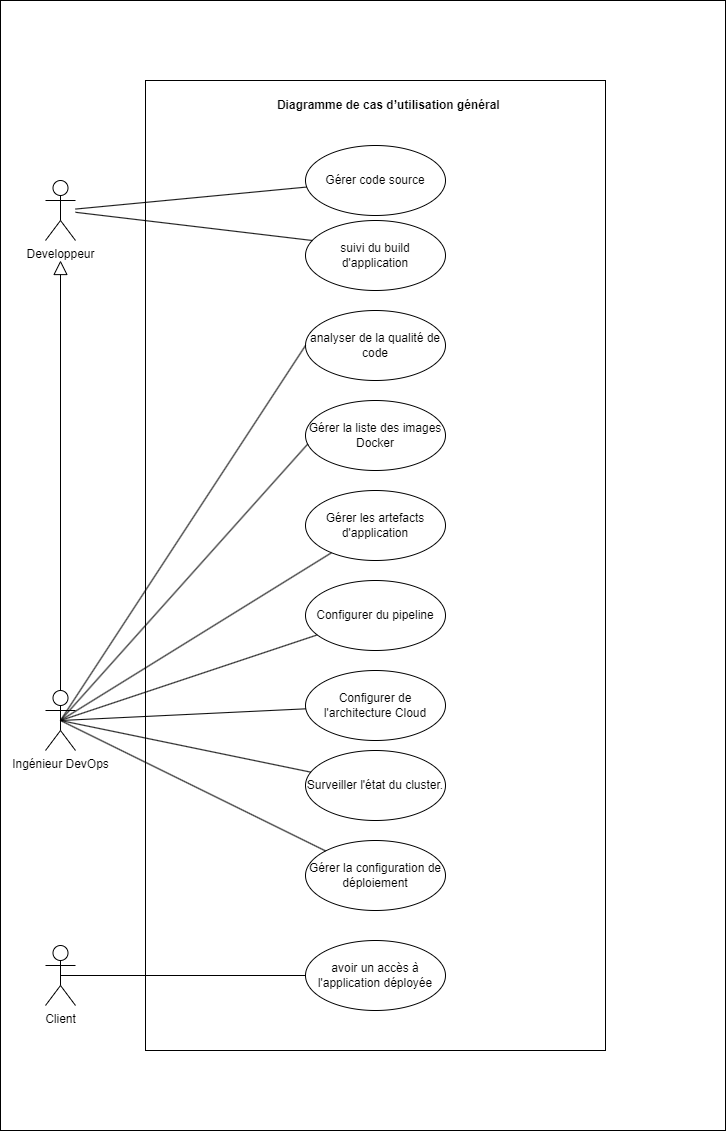
\includegraphics[width=12cm]{Use case.drawio.png}

  \end{center}
  
  \caption{Diagramme de cas d'utilisation Globale}
\end{figure}


Dans ce qui suit , le raffinnement des différents cas d'utilisation.\\[0.2cm]
\subsection{\Large Cas d’utilisation "Gérer code source"}
Dans cette section, nous décrirons de façon détaillée ce cas d'utilisation.\\\texttt{}\\[0.01cm]

\begin{figure}[H]
  \begin{center}
  
      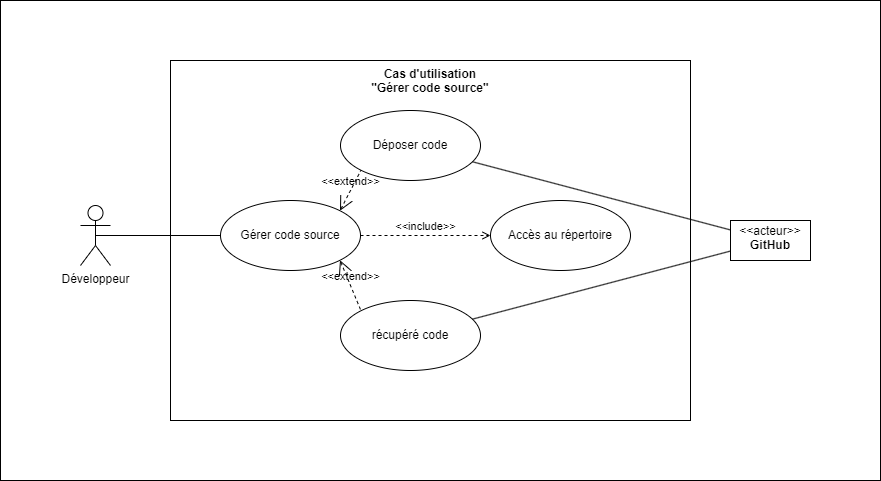
\includegraphics[width=15cm]{usecase1.drawio.png}

  \end{center}
  
  \caption{Cas d'utilisation:Gérer code source }
\end{figure}

Pour expliquer  le diagramme de cas d’utilisation, nous représentons la description textuelle du principales fonctionnalités mentionnées ci-dessus (Voir tableau 2.2): \\

\begin{center}
 \begin{table}[H] 
 \centering
 \resizebox{1.1\textwidth}{!}{%
 \begin{tabular}{|c|p{13cm}|}
 \hline
 Titre & Gérer code source\\
 \hline
 Acteur & Développeur \\
 \hline
 Description & le développeur peut déposer ou récupérer le code à travers le command "pull" ou "push".\\
 \hline
 Pré conditions & Une connexion établie entre le PC du développeur et le répertoire Git de l'application. \\
 \hline
 Post conditions & Code envoyé au répertoire git. \\
 \hline 
 \multirow{3}{*}{Scénario nominal} & 1- Avoir un accès au répertoire. \\
 & 2 - Gérer code source. \\
 & 3 - Déposer ou récuperer  le code dans le répertoire github. \\
 \hline
 \multirow{3}{*}{Scénario alternatif} & 1- La connexion entre la machine du développeur et Git ne peut pas être établie. \\
 & 2 - Le code ne peut pas être envoyé. \\
 & 3 - Retour à l'étape 1 du Scénario nominal. \\ 
 \hline
 \end{tabular}%
 }
 \caption{Description de cas d’utilisation:Gérer code source}
 \end{table}
\end{center}


   \subsection{\Large Cas d’utilisation "Suivi de la build d'application"}

Dans cette section, nous décrirons de façon détaillée ce cas d'utilisation.\\\texttt{}\\[0.01cm]

\begin{figure}[H]
  \begin{center}
  
      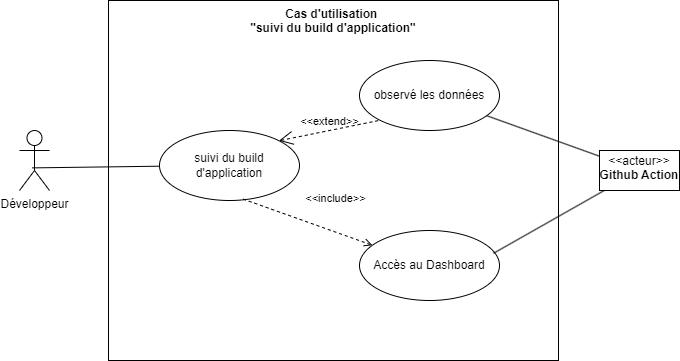
\includegraphics[width=15cm]{UseCase2.drawio.png}

  \end{center}
  
  \caption{Cas d'utilisation:Suivi la build d'application }
\end{figure}

Pour expliquer  le diagramme de cas d’utilisation, nous représentons la description textuelle des principales fonctionnalités mentionnées ci-dessus(voir tableau 2.3 ) : \\
\begin{center}
   \begin{table}[H]  
     \centering
     \resizebox{1.1\textwidth}{!}{%
     \begin{tabular}{|c|p{13cm}|}
      \hline
      Titre &  Suivi du build de l'application\\
      \hline
      Acteur & Développeur \\
      \hline
      Description & Le développeur peut suive la construction d'application pour connaître si la modification ajoutée au code source est valide ou non.\\
      \hline
      Pré conditions & Une connexion  établie entre le développeur et Github actions. \\
      \hline
      Post conditions & Affichage de Dashboard Github Actions. \\
      \hline 
      \multirow{3}{*}{Scénario nominal} & 1- Avoir un accès au Dashbord \\ 
      & 2- Suivi du build de l'application \\
      & 3- L'observation de la construction de l'application rapporte un succès.\\
      \hline
      \multirow{2}{*}{Scénario alternatif} & 1 - La connexion entre développeur et Github Actions ne peut pas être établie. \\
      & 2 - Retour à l'étape 1 du Scénario nominal.\\ 
      \hline
      \end{tabular}%
     }
   \caption{Description de cas d’utilisation:Suivi du build de l'application}
   \end{table}
   \end{center}
   \subsection{\Large Cas d'utilisation"Gérer la configuration de déploiement"}
    Dans cette section, nous décrirons de façon détaillée ce cas d'utilisation(voir figure 2.4).\\\texttt{}\\[0.01cm]
   
   \begin{figure}[H]
    \begin{center}
    
        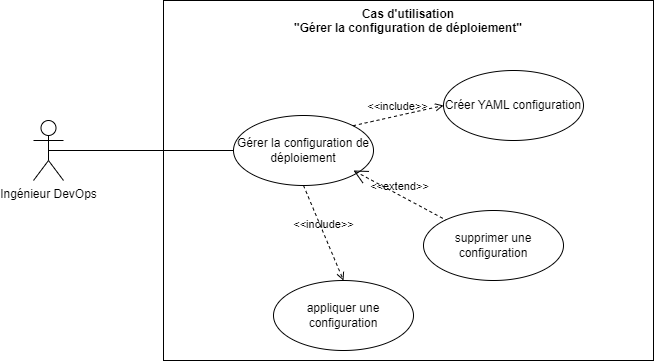
\includegraphics[width=15cm]{UserCase3.drawio.png}
  
    \end{center}
    
    \caption{Cas d'utilisation:Gérer la configuration de déploiement}
  \end{figure}
   
   Pour expliquer  le diagramme de cas d’utilisation, nous représentons la description textuelle des principales fonctionnalités mentionnées ci-dessus (voir table 2.4)  : \\
   \begin{center}
      \begin{table}[H]  
        \centering
        \resizebox{1.1\textwidth}{!}{%
        \begin{tabular}{|c|p{13cm}|}
         \hline
         Titre & Gérer la configuration de déploiement\\
         \hline
         Acteur & Ingénieur DevOps \\
         \hline
         Description & L'ingénieur DevOps gére la configuration de déploiement pour assurer la meilleure performance du cluster.\\
         \hline
         Pré conditions & Fonctionnement correct du cluster EKS. \\
         \hline
         Post conditions & Une configuration ou modification d'une configuration déjà existante. \\
         \hline 
        \multirow{2}{*}{Scénario nominal} & 1 - Lancer la configuration  du déploiement. \\
        & 2 - La configuration est lancée dans le contrôle plane d'EKS.\\
         \hline
        \multirow{3}{*}{Scénario alternatif} & 1 - La  nouvelle configuration n'est pas flexible. \\
        & 2 - Un problème apparaît causé par la nouvelle configuration.  \\
        & 3 - Retour à l'étape 1 du Scénario nominal.\\
         \hline
         \end{tabular}%
         }
      \caption{Description de cas d’utilisation:Gérer la configuration de déploiement}
      \end{table}
      \end{center}
      \subsubsection{\Large Cas utilisation"Gérer liste des images Docker"}
       
      Dans cette section, nous décrirons de façon détaillée le cas d'utilisation (voir figure 2.5).\\\texttt{}\\[0.01cm]
      
      \begin{figure}[H]
        \begin{center}
        
            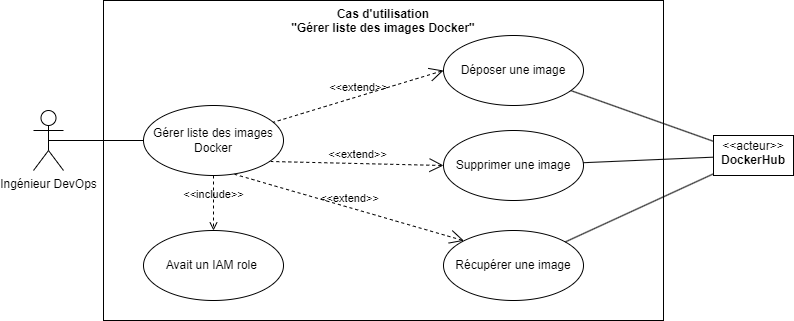
\includegraphics[width=15cm]{usecase5.drawio.png}
      
        \end{center}
        
        \caption{Cas d'utilisation:Gérer liste des images Docker}
      \end{figure}
      
      Pour expliquer  le diagramme de cas d’utilisation, nous représentons la description textuelle des principales fonctionnalités mentionnées ci-dessus (voir table 2.5) : \\
      \begin{center}
         \begin{table}[H]  
           \centering
           \resizebox{1.1\textwidth}{!}{%
           \begin{tabular}{|c|p{13cm}|}
            \hline
            Titre & Gérer liste des images Docker\\
            \hline
            Acteur & Ingénieur DevOps \\
            \hline
            Description & L'ingénieur DevOps gére la liste des images Docker\\
            \hline
            Pré conditions & Connexion au répertoire de l'application dans ECR. \\
            \hline
            Post conditions & Une image modifiée ,supprimée ou ajoutée. \\
            \hline 
           \multirow{4}{*}{Scénario nominal} & 1 - Se connecter ou l'enregistremementc de l'image n'est pas valide. \\
           & 2 -  Configurer liste des images Docker .\\
           & 2 - Déposer ou récuperer le code dans le répertoire ECR. \\
           & 3 - L'image est enregistrée dans la répertoire ECR.\\
            \hline
            \multirow{3}{*}{Scénario alternatif} & 1 - La connexion ou l'enregistrement de image n'est pas valide.  \\
            & 2 - Echec du dépose ou  récuperation l'image Docker .\\
            & 3 - Retour à l'étape 1 du Scénario nominal.\\
            \hline
            \end{tabular}%
           }
         \caption{Description de cas d’utilisation:Gérer liste des images Docker}
         \end{table}
         \end{center} 
         
      \subsection{\Large Cas utilisation"Gérer les artefacts d'application"}

         Dans cette section, nous décrirons de façon détaillée ce cas d'utilisation (voir figure 2.6).\\\texttt{}\\[0.01cm]
         
         \begin{figure}[H]
          \begin{center}
          
              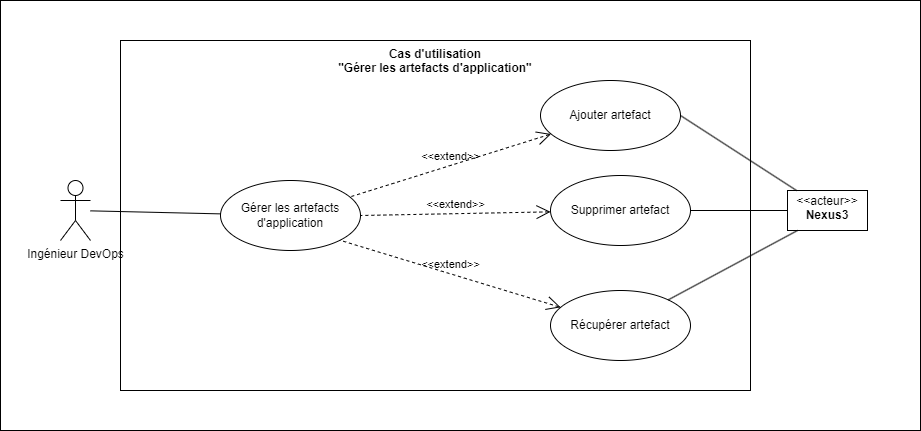
\includegraphics[width=15cm]{Usecase6.drawio.png}
        
          \end{center}
          
          \caption{Cas d'utilisation:Gérer les artefacts d'application}
        \end{figure}
         
         Pour expliquer  le diagramme de cas d’utilisation, nous représentons la description textuelle des principales fonctionnalités mentionnées ci-dessus ( voir table 2.6): \\
         \begin{center}
            \begin{table}[H]  
              \centering
              \resizebox{1.1\textwidth}{!}{%
              \begin{tabular}{|c|p{13cm}|}
               \hline
               Titre & Gérer les artefacts de l'application\\
               \hline
               Acteur & Ingénieur DevOps \\
               \hline
               Description & L'ingénieur DevOps gére la liste des artefacts pour assurer l'enregistrement de différentes versions d'application.\\
               \hline
               Pré conditions & Connexion HTTP au serveur Nexus. \\
               \hline
               Post conditions & Une répertoire avec les différentes artefacts de l'application.  \\
               \hline 
               \multirow{3}{*}{Scénario nominal} & 1 - Saisir les données d'authetification pour accéder à l'interface .\\
               & 2 - Configurer les artifacts d'application . \\
               & 3 - la connexion est réussite et la modification dans le répertoire est enregistrée dans Nexus .\\
               \hline
               \multirow{2}{*}{Scénario alternatif} & 1 - La connexion échoue ou la modification n'est pas enregistrée.  \\
               & 2 - Retour à l'étape 1 du Scénario nominal. \\
               \hline
               \end{tabular}%
              }
            \caption{Description de cas d’utilisation:Gérer les artefacts d'application}
            \end{table}
            \end{center}
  \section{\fontfamily{ptm}\selectfont\Large  Conception du système}

Dans ce qui suit,nous allons présenter les différents diagrammes de conception. \\[0.1cm]
            \subsection{\fontfamily{ptm}\selectfont\Large Diagramme de séquence global}
         Les diagrammes de séquences sont la représentation graphique des interactions entre les acteurs et le système selon un ordre chronologique\cite{14}(voir figure 3.1).
            % \begin{figure}[H]
            %   \begin{center}
            %   \centering
            %       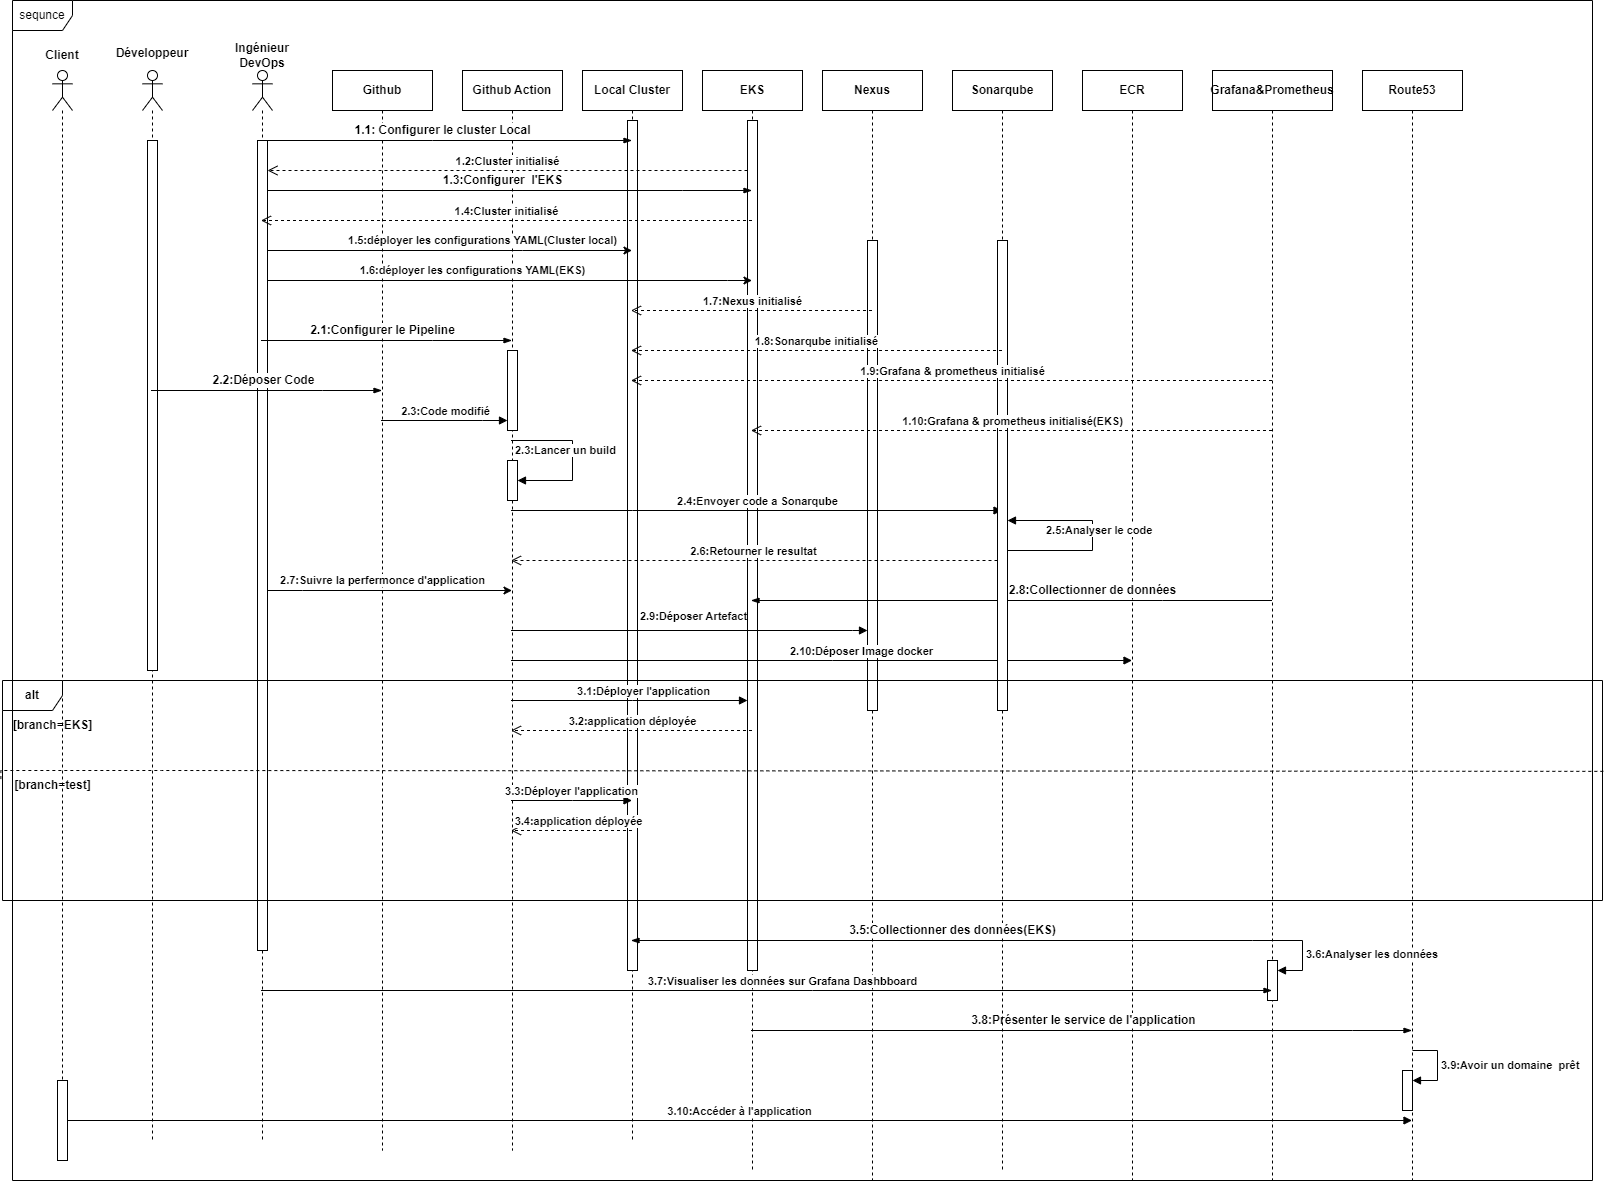
\includegraphics[height=25cm,width=18cm]{Squence.drawio.png}
            
            %   \end{center}
              
            %   \caption{Diagramme de séquence global}
            
            % \end{figure}
            \begin{landscape}
              \begin{figure}[htbp]
                \centering
                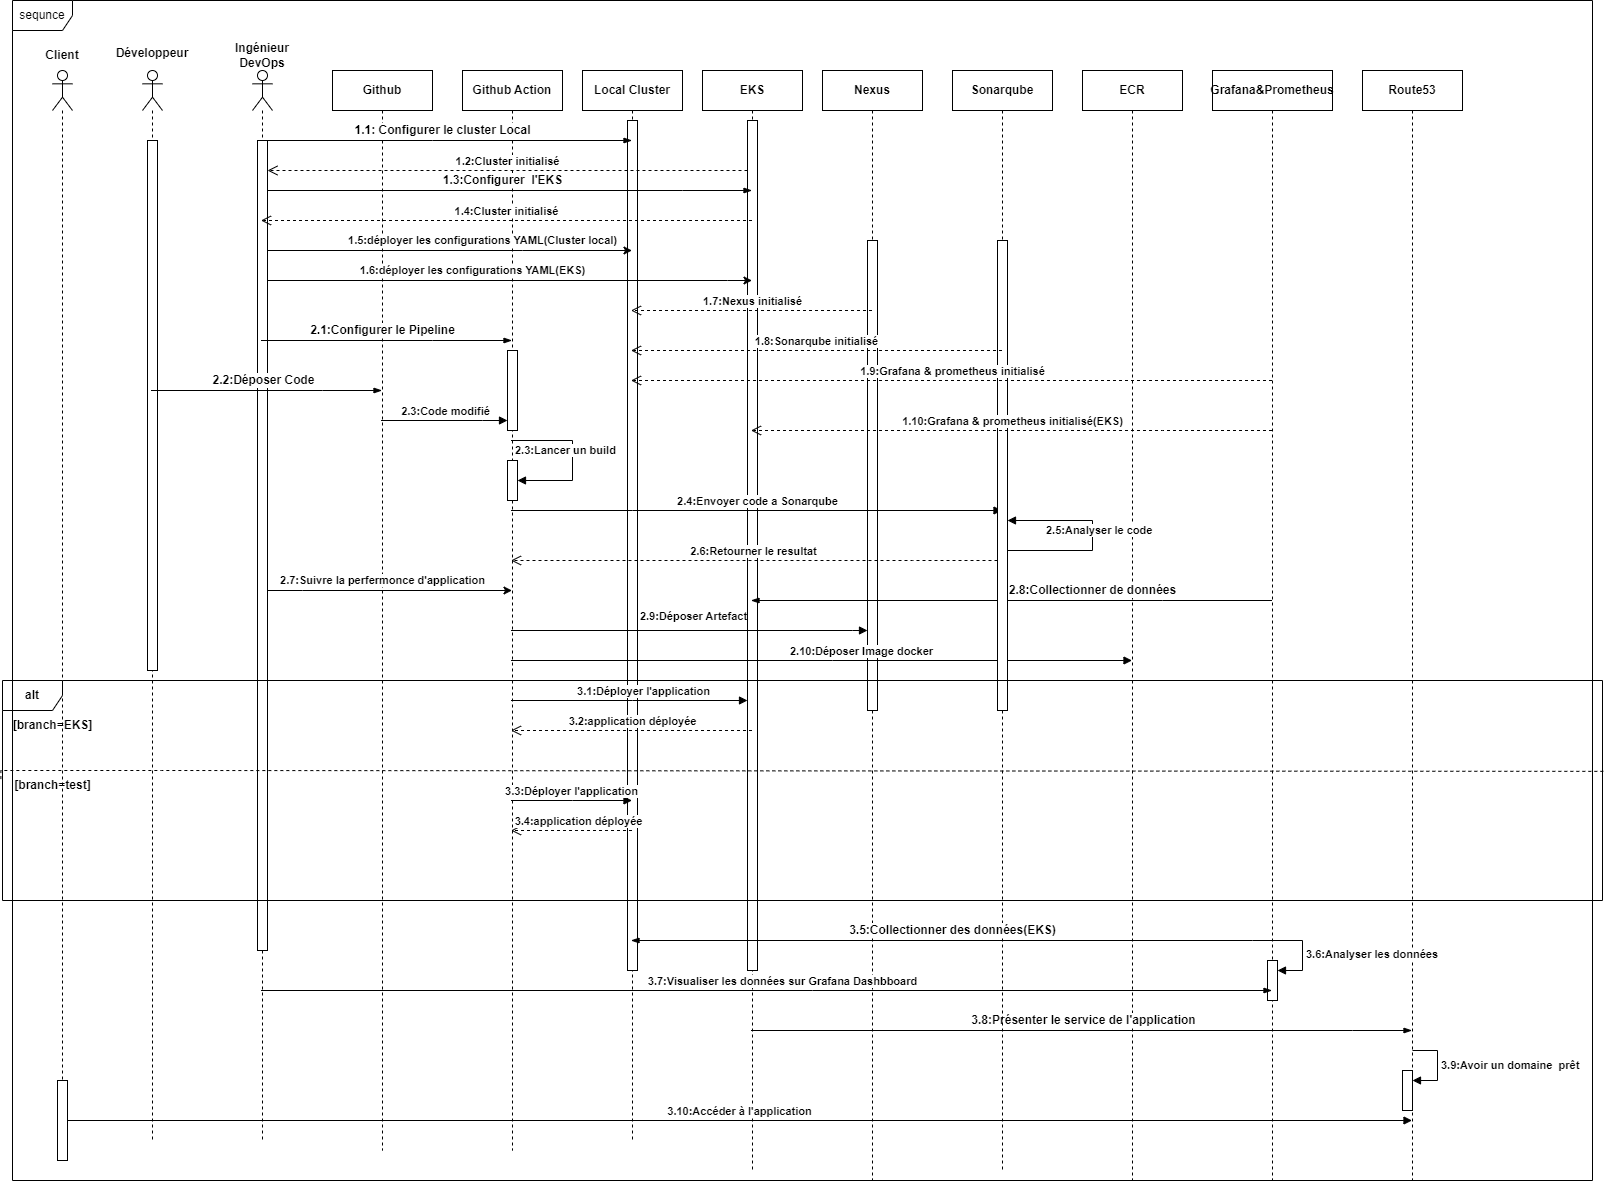
\includegraphics[width=24cm]{Squence.drawio.png} % Replace with your photo filename
                \caption{Diagramme de séquence Global}
              
              \end{figure}
            \end{landscape}
            \subsection{\fontfamily{ptm}\selectfont\Large Diagramme de séquence Détaillé}
            Pour une meilleure présentation et illustration de projet nous allons décrire les différents cas d'utilisations principaux avec leurs diagrammes de séquence détaillés.
            \subsubsection{\fontfamily{ptm}\selectfont\scalefont{1.35}Diagramme de séquence «Configuration de l'architecture cloud»}
            Nous détaillons ci-dessous les interactions du diagramme de séquence « Configuration de l'architecture cloud » 
            \begin{figure}[H]
                \begin{center}
                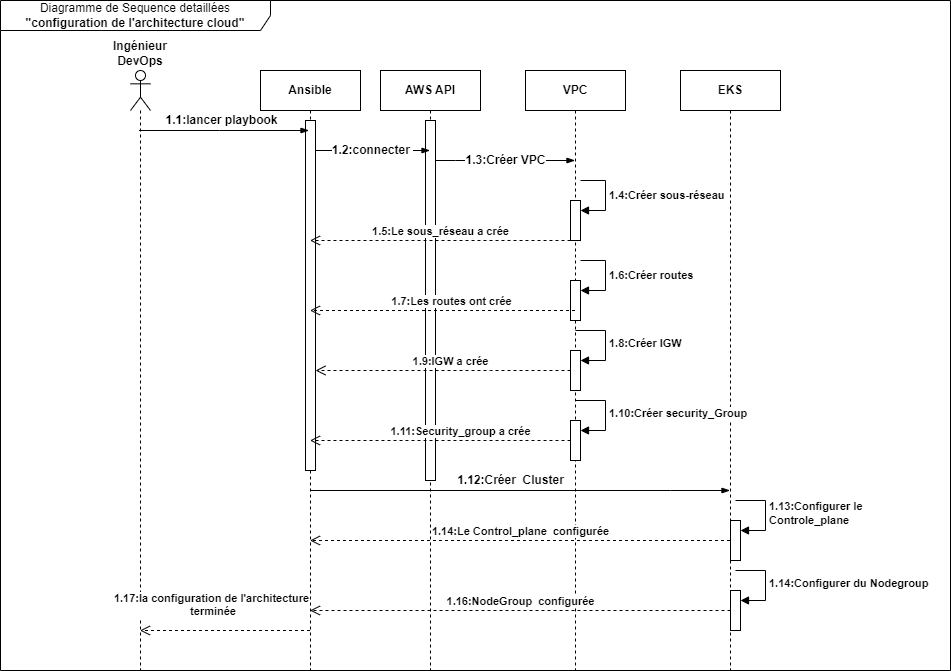
\includegraphics[height=15cm,width=18cm]{seqd.drawio.png}
                \end{center}
                \caption{Diagramme de séquence « Configuration de l'architecture cloud » }
                %\floatfoot{Source: (Citation command)}
                % avec le package "floatrow"
                \end{figure}
                \subsubsection{\fontfamily{ptm}\selectfont\Large Diagramme de séquence « Configuration de cluster local » }
                Nous détaillons ci-dessous les interactions de diagramme de séquence « Configuration de cluster local » (voir figure 3.3). 
                \begin{figure}[H]
                    \begin{center}
                    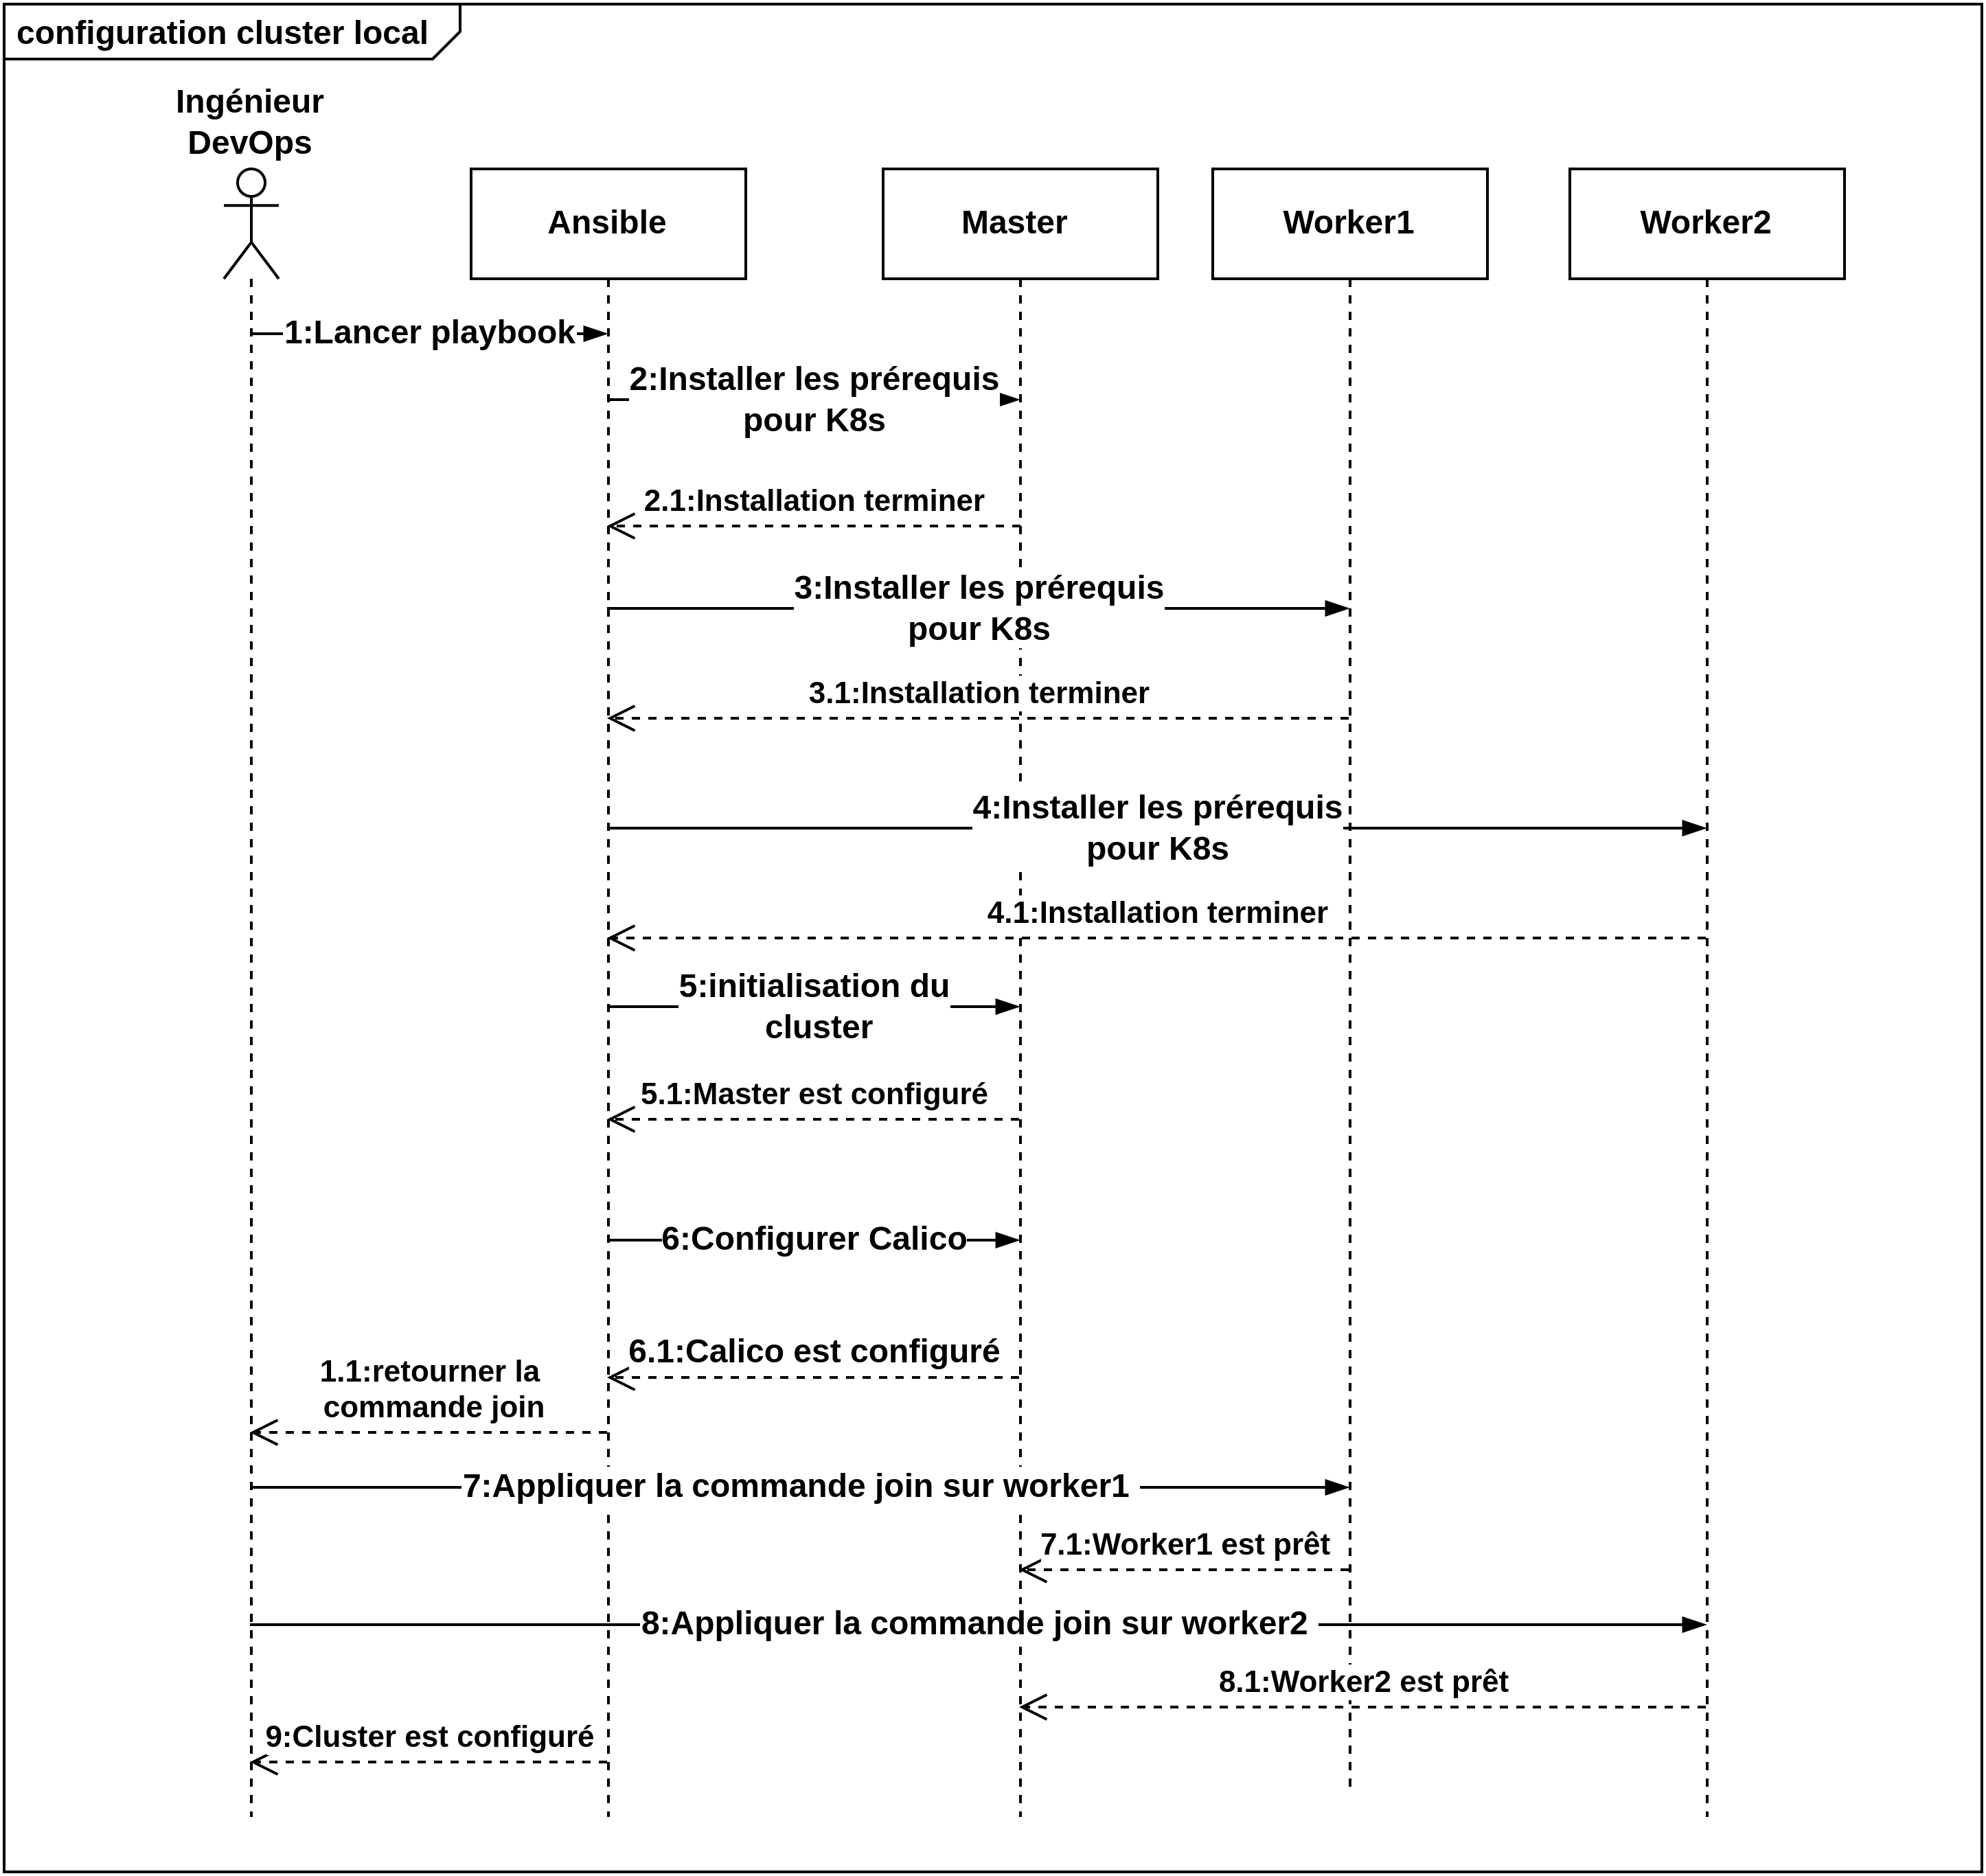
\includegraphics[height=15cm,width=18cm]{SEQCLUSTER.png}
                    \end{center}
                    \caption{Diagramme de séquence « Configuration de cluster local »}
                    %\floatfoot{Source: (Citation command)}
                    % avec le package "floatrow"
                    \end{figure}\subsubsection{\fontfamily{ptm}\selectfont\Large Diagramme de séquence « Configuration du pipeline » }
            Nous détaillons ci-dessous les interactions de diagramme de séquence « Configuration du pipeline » (voir figure 3.4)  .
            \begin{figure}[H]
                \begin{center}
                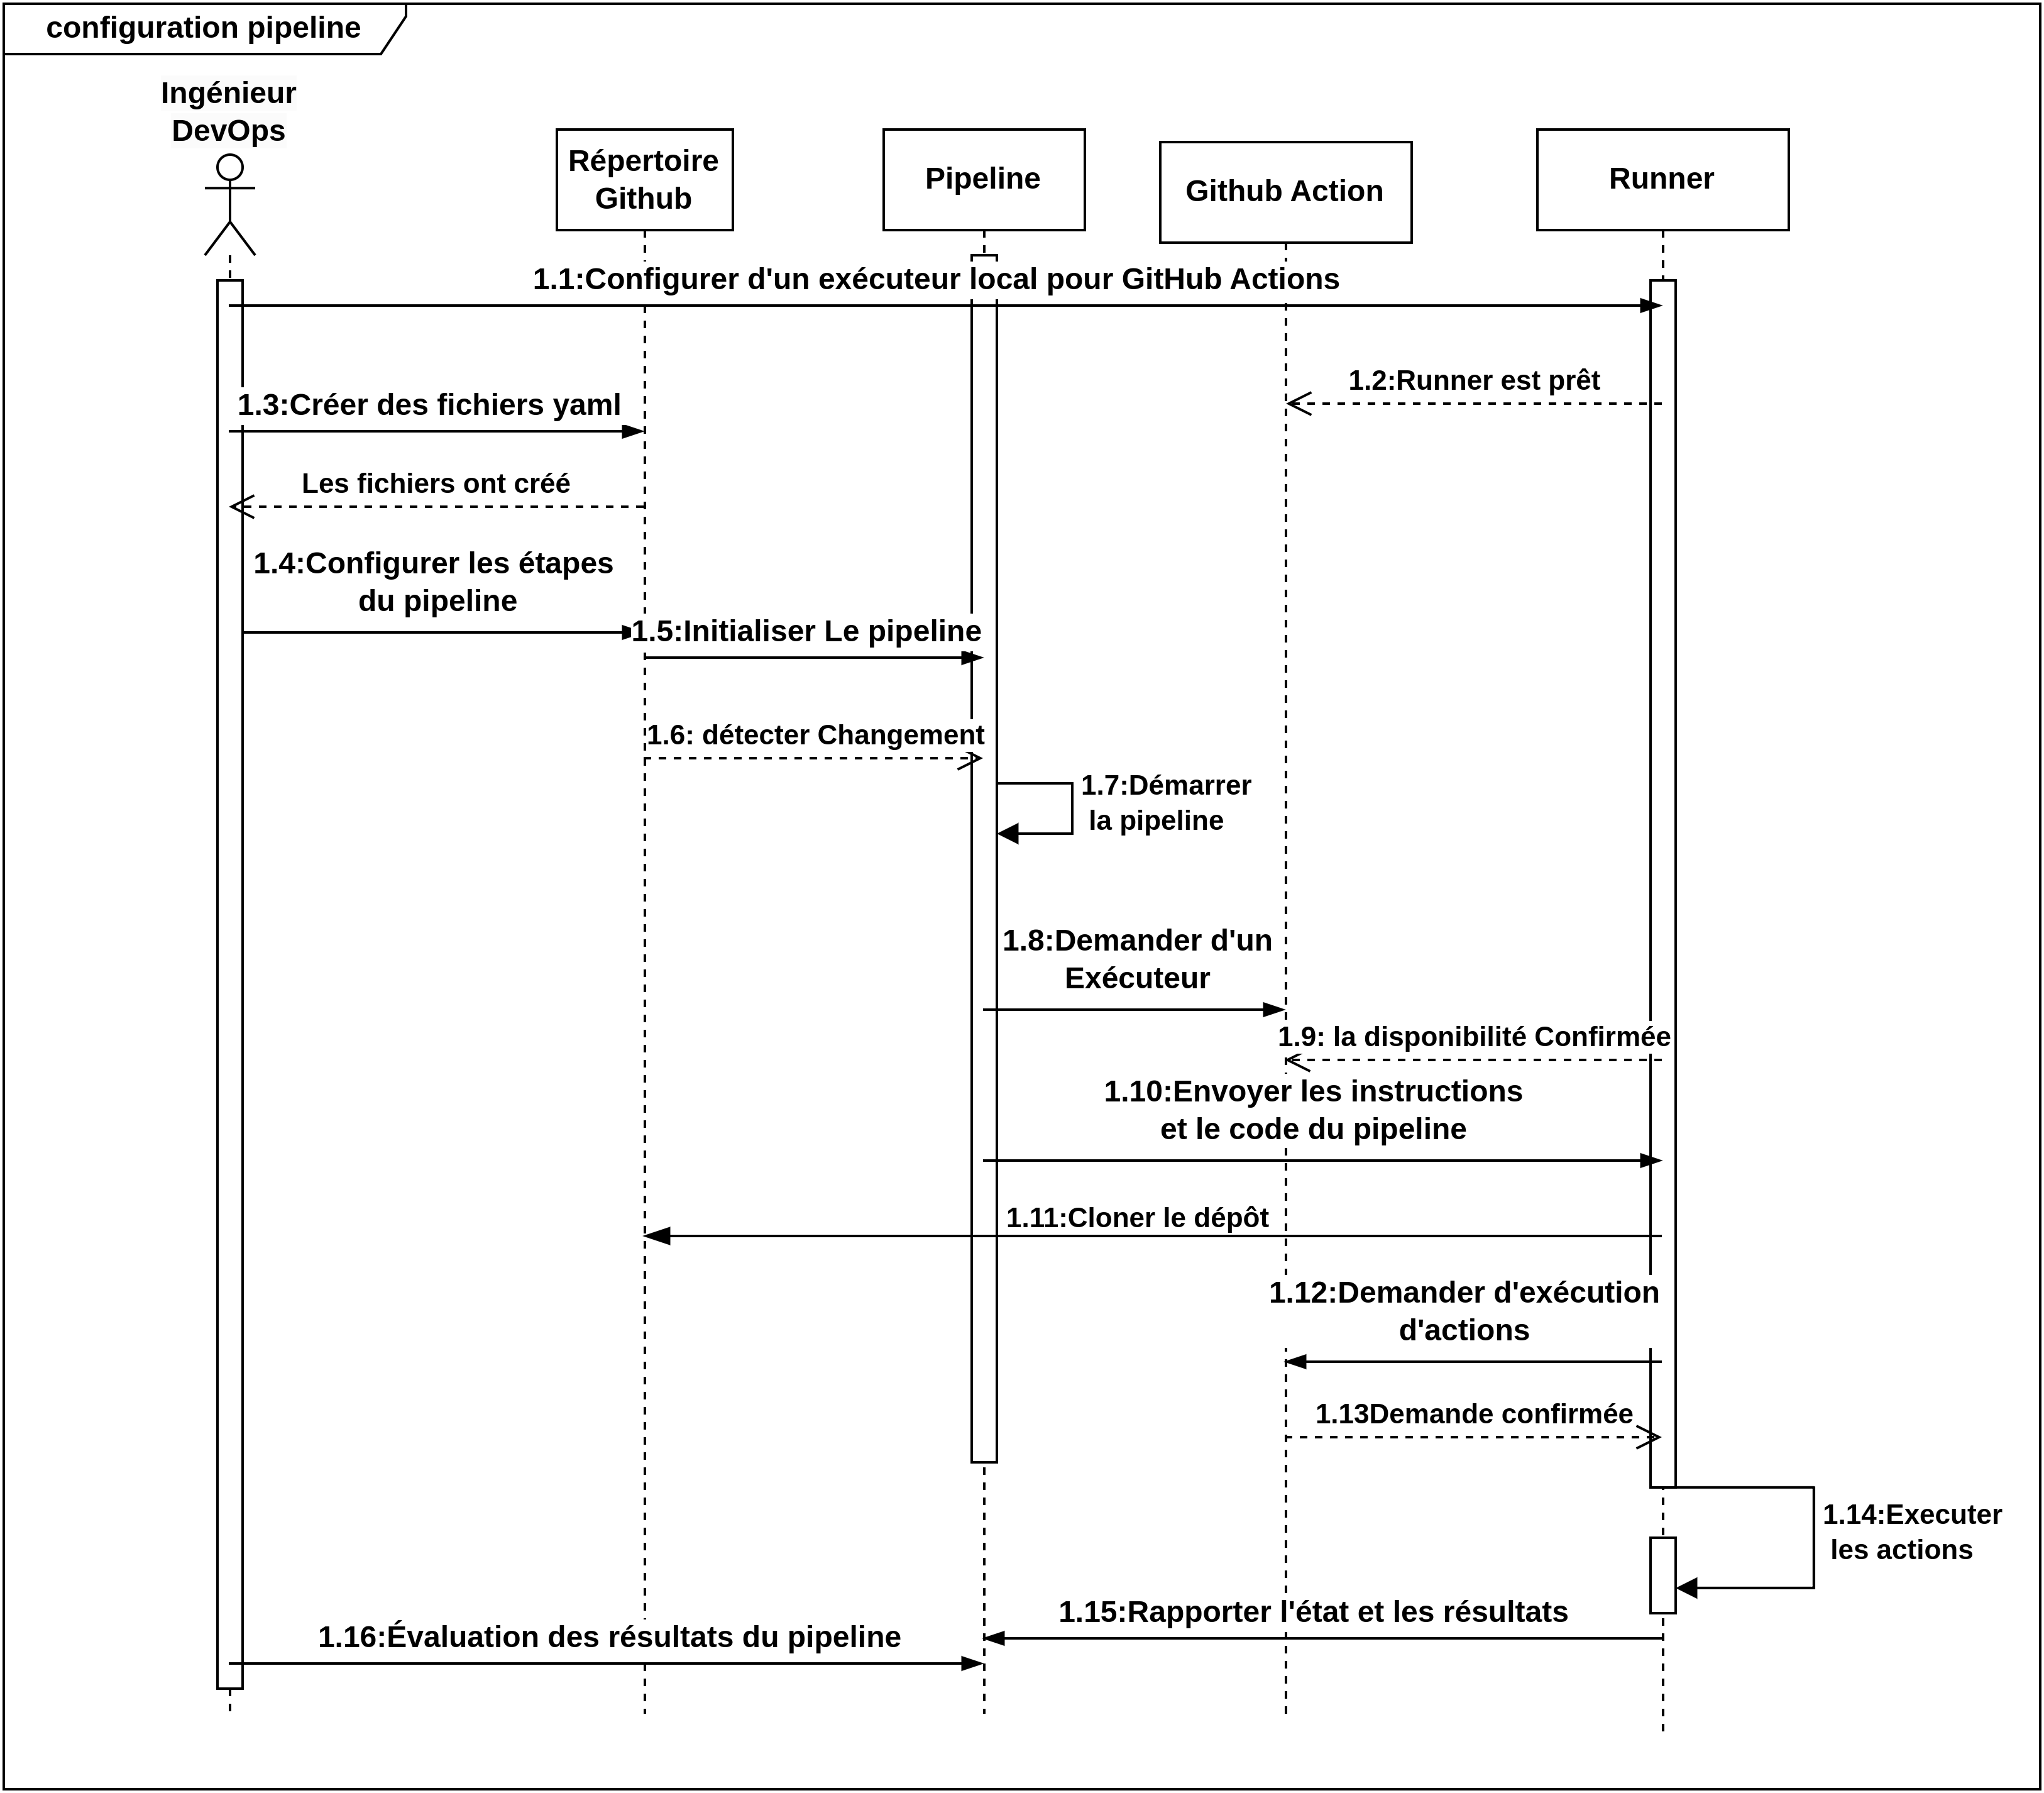
\includegraphics[height=15cm,width=18cm]{SEQPIPELINE.png}
                \end{center}
                \caption{Diagramme de séquence « Configuration du pipeline »}
                %\floatfoot{Source: (Citation command)}
                % avec le package "floatrow"
                \end{figure}
            
\subsection{\fontfamily{ptm}\selectfont\Large Diagramme de classe}
 Le diagramme de classes est un schéma utilisé en génie logiciel pour présenter les classes et les interfaces du système ainsi que leurs relations.La figure ci-dessous représente le 
diagramme de classe de notre travail(voir figure 4.5)\cite{13}.
\begin{figure}[H]
  \begin{center}
  
      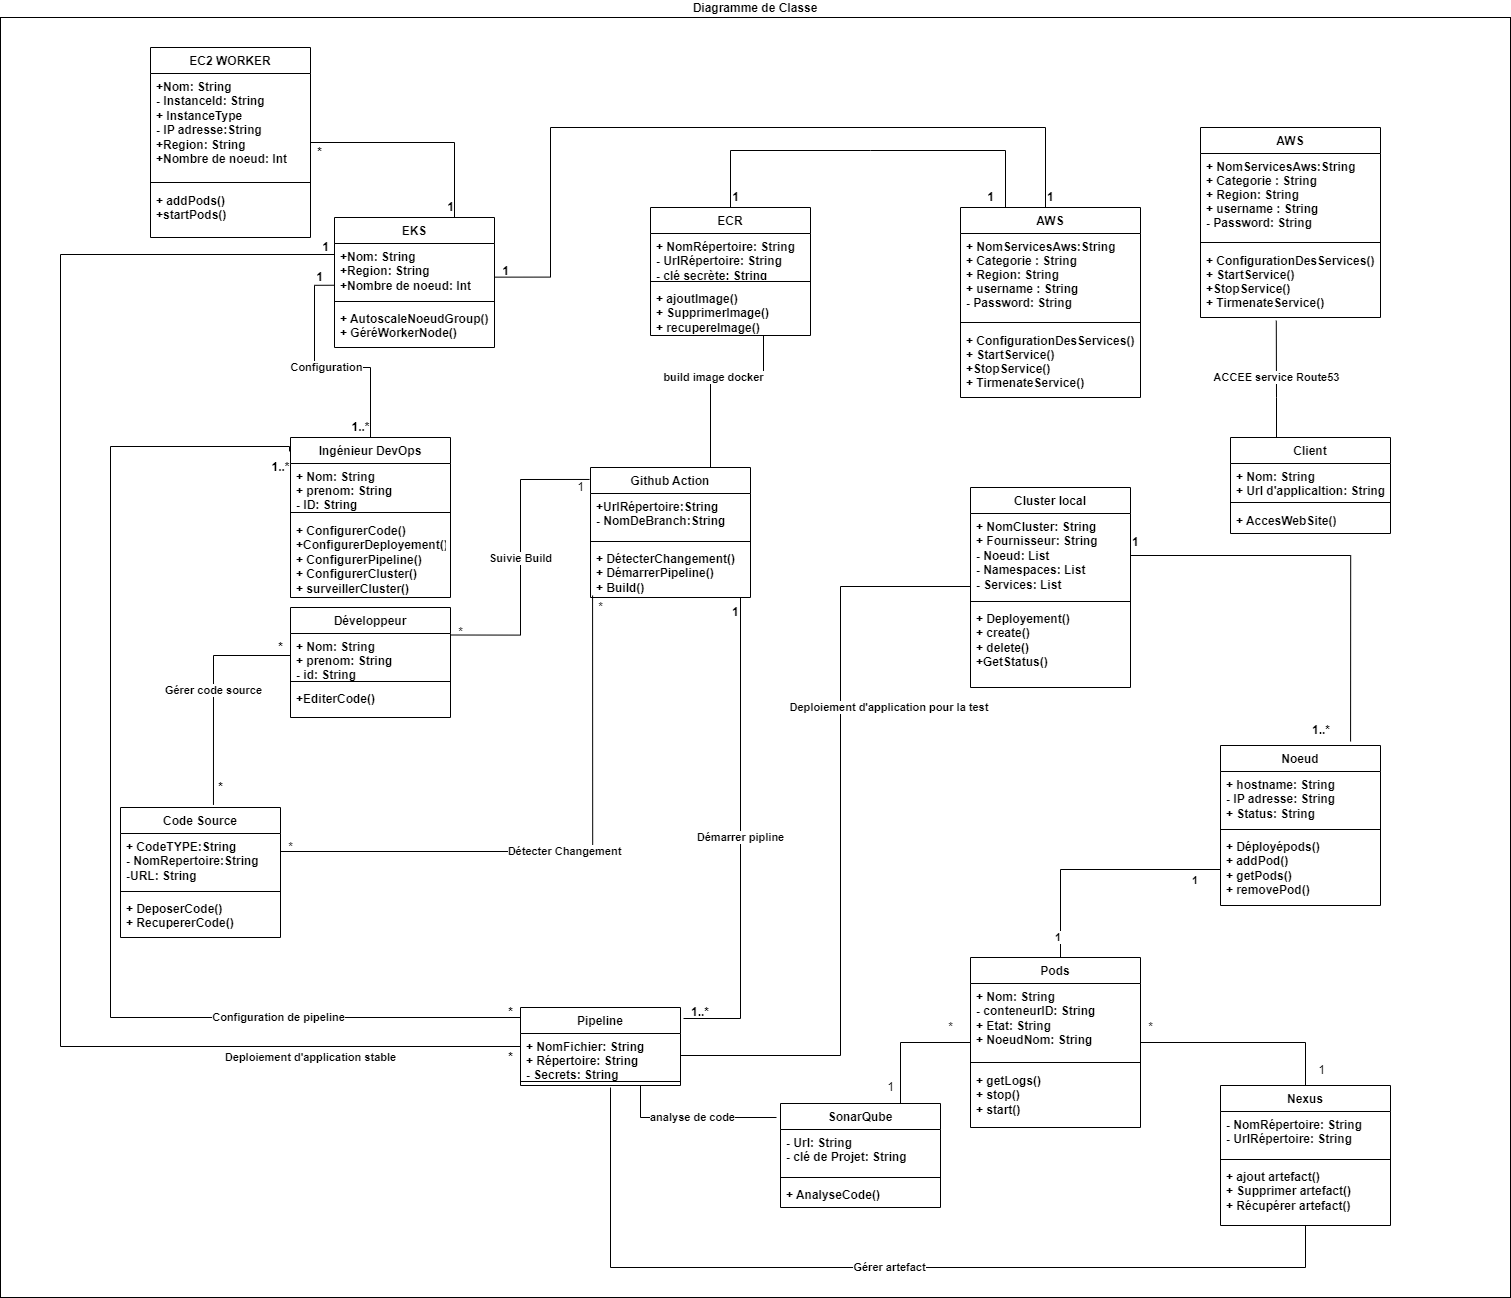
\includegraphics[width=18cm,height=18cm]{ClassDiagram.drawio.png}

  \end{center}
  
  \caption{Diagramme de classe global}
\end{figure}
\subsection{\fontfamily{ptm}\selectfont\Large Diagramme de déploiement}
 Un diagramme de déploiement est une vue statique qui sert à représenter l'utilisation de l'infrastructure physique par le système et la manière dont les composants du système sont répartis ainsi que leurs relations entre eux (voir figure 4.6)\cite{15}.
\begin{figure}[H]
  \begin{center}
  
    \fbox{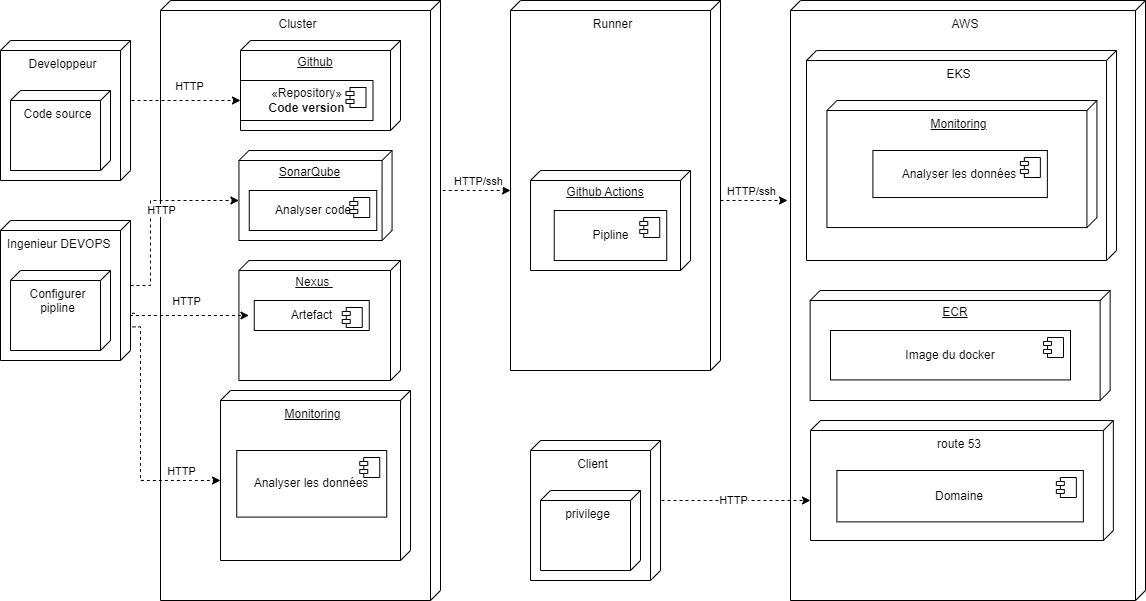
\includegraphics[height=18cm,width=18cm]{deploiment-1.drawio.png}}

  \end{center}
  
  \caption{Diagramme de déploiement global}
\end{figure}
%\section{\fontfamily{ptm}\selectfont\Large Méthodologie de conception}
%\textsf{\fontfamily{ptm}\selectfont\scalefont{1.3}Il est indispensable de choisir un méthodologie de développement  et nous avons choisir la méthodologie (CI/CD). \\
%L’Intégration Continue (CI) et la Livraison Continue (CD) regroupent un ensemble de principes et de pratiques permettant aux équipes de développement d’apporter des changements au code informatique de façon plus fiable et plus fréquente.\\
%L’implémentation du CI/CD est au coeur des méthodologies de développement agile et DevOps. Elle permet aux équipes de développement logiciel de se focaliser sur les besoins de l’entreprise, la qualité du code et la cybersécurité. Les étapes de déploiement sont automatisées.Ainsi , les pipelines CI/CD permettent aux entreprises d’améliorer fréquemment leurs applications tout en s’appuyant sur un processus de livraison fiable. La standardisation des builds, les tests, l’automatisation du déploiement laissent les équipes se focaliser sur l’amélioration des applications plutôt que sur des détails techniques.\\
%Cette pratique est idéale pour la méthode DevOps, car elle évite un mauvais alignement entre des développeurs désirant pousser le code trop fréquemment et les équipes ops en quête de stabilité des applications. L’automatisation permet de pousser des changements de code plus fréquemment, tandis que les configurations standardisées et le testing continu améliorent la stabilité.\cite{20}(Voir figure 4.7)}\\[0.1cm]
%\begin{figure}[H]
%  \begin{center}
%  
%      \fbox{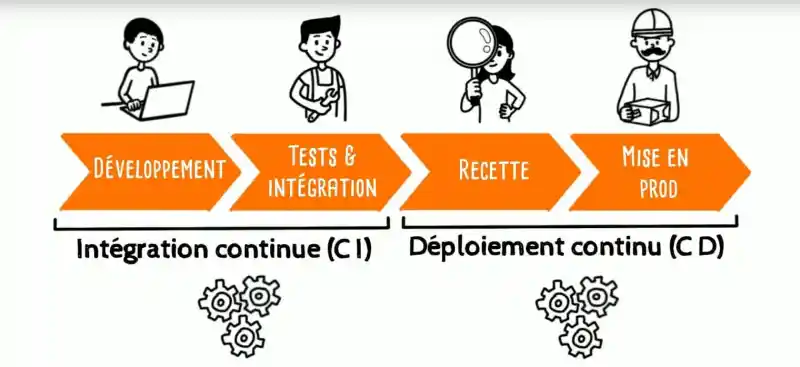
\includegraphics[height=11cm,width=15cm]{CI-CD-fonctionnement.png}}
%
%  \end{center}
%  
%  \caption{Diagramme de déploiement global}
%\end{figure}
\section{\fontfamily{ptm}\selectfont\Large Architecture technologique de la solution}
 Dans cette partie nous allons présenter l'architecture globale de notre projet(voir figure 3.8).
\begin{landscape}
  \begin{figure}[htbp]
    \centering
  \includegraphics[width=25cm,height=17cm]{GLOBALAWS.png}  
    \caption{Architecture global}
  \end{figure}
\end{landscape}
 Pour plus de clarté, nous allons diviser notre architecture globale en deux parties.\\
\indent--Partie local: \\[0.02cm]
La figure (figure: 3.9) représente les ressources utiliser localement dans le projet.


\begin{figure}[H]
\centering
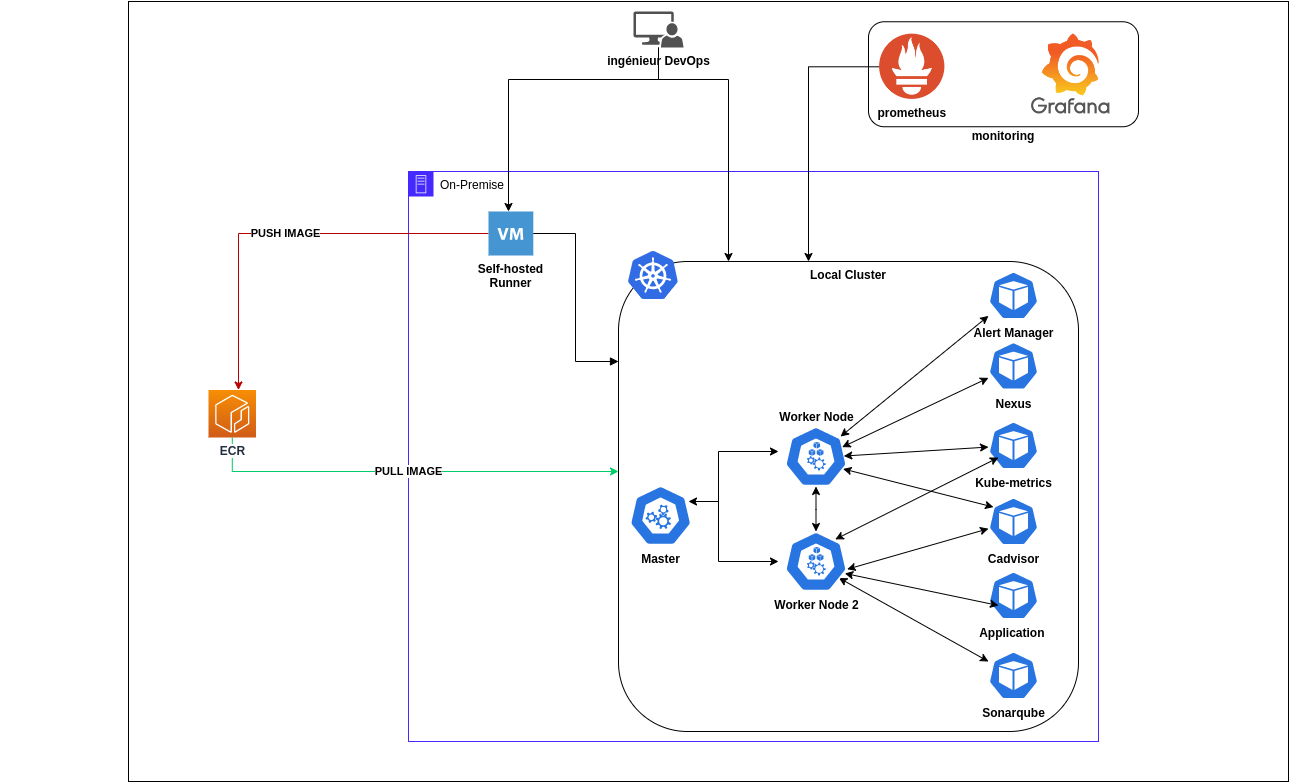
\includegraphics[width=15cm,height=12.5cm]{LOCAL.drawio.png}

  \caption{Partie local}
\end{figure}

\begin{tikzpicture}
  \draw[fill=black] (2,2) circle (2pt);
\end{tikzpicture} 
 Le cluster local dans l’architecture globale fonctionne comme un environnement dédié pour les tests et le développement. Il est configuré et géré par l'ingénieur devops, qui dispose des droits et des permissions nécessaires. Le cluster local est composé de plusieurs composants clés qui facilitent le développement efficace et tester les flux de travail.     \\[0.02cm]
 \indent
 \begin{tikzpicture}
  \draw[fill=black] (2,2) circle (2pt);
\end{tikzpicture} 
 Dans le cluster local, plusieurs nœuds ou machines virtuelles sont fournis pour créer un environnement similaire à la configuration de production. Ces nœuds exécutent des conteneurs ou d’autres outils de test, permettant possible de simuler le comportement et les performances de l’environnement de production localement. L’ingénieur de devons supervise la configuration et la gestion du cluster local, en assurant sa disponibilité et sa stabilité pour les activités de test et de développement.\\[0.02cm]
 \indent
 \begin{tikzpicture}
  \draw[fill=black] (2,2) circle (2pt);
\end{tikzpicture} 
 Pour surveiller le cluster local, l’ingénieur devops déploie Grafana et Prometheus, qui fournissent des informations précieuses sur les performances et la santé du cluster. Ces outils de surveillance permettent de suivre l’utilisation des ressources, de détecter et de résoudre les problèmes rapidement, ce qui permet l’amélioration continue et l’optimisation de l’environnement de test local.\\[0.02cm]
 \indent
 \begin{tikzpicture}
  \draw[fill=black] (2,2) circle (2pt);
\end{tikzpicture}
 L’ingénieur devops configure également un exécuteur local pour GitHub Actions. Cet exécuteur permet de déclencher des pipelines. Dans le cas de la branche principale, un pipeline démarre et les actions de déploiement nécessaires sont exécutées sur le cluster local. Cela permet l'ingénieur devops de valider les changements dans un environnement qui ressemble beaucoup à la configuration de production, assurant robustesse et fiabilité.
 \\[0.02cm]
 \indent
 \begin{tikzpicture}
  \draw[fill=black] (2,2) circle (2pt);
\end{tikzpicture}
L’ingénieur de devops configure l’environnement pour extraire les images de conteneurs d’un dépôt ECR privé, qui stocker et gérer les images de conteneurs. Les images du dépôt sont séparées par des versions telles que 1.0.0 , 0.0.1 pour les tests.
 
 
\indent{\fontfamily{ptm}\selectfont\scalefont{1.3}--Partie AWS:} \\
La figure ci-dessous représente les ressources cloud utiliser dans notre projet.
\begin{figure}[H]


  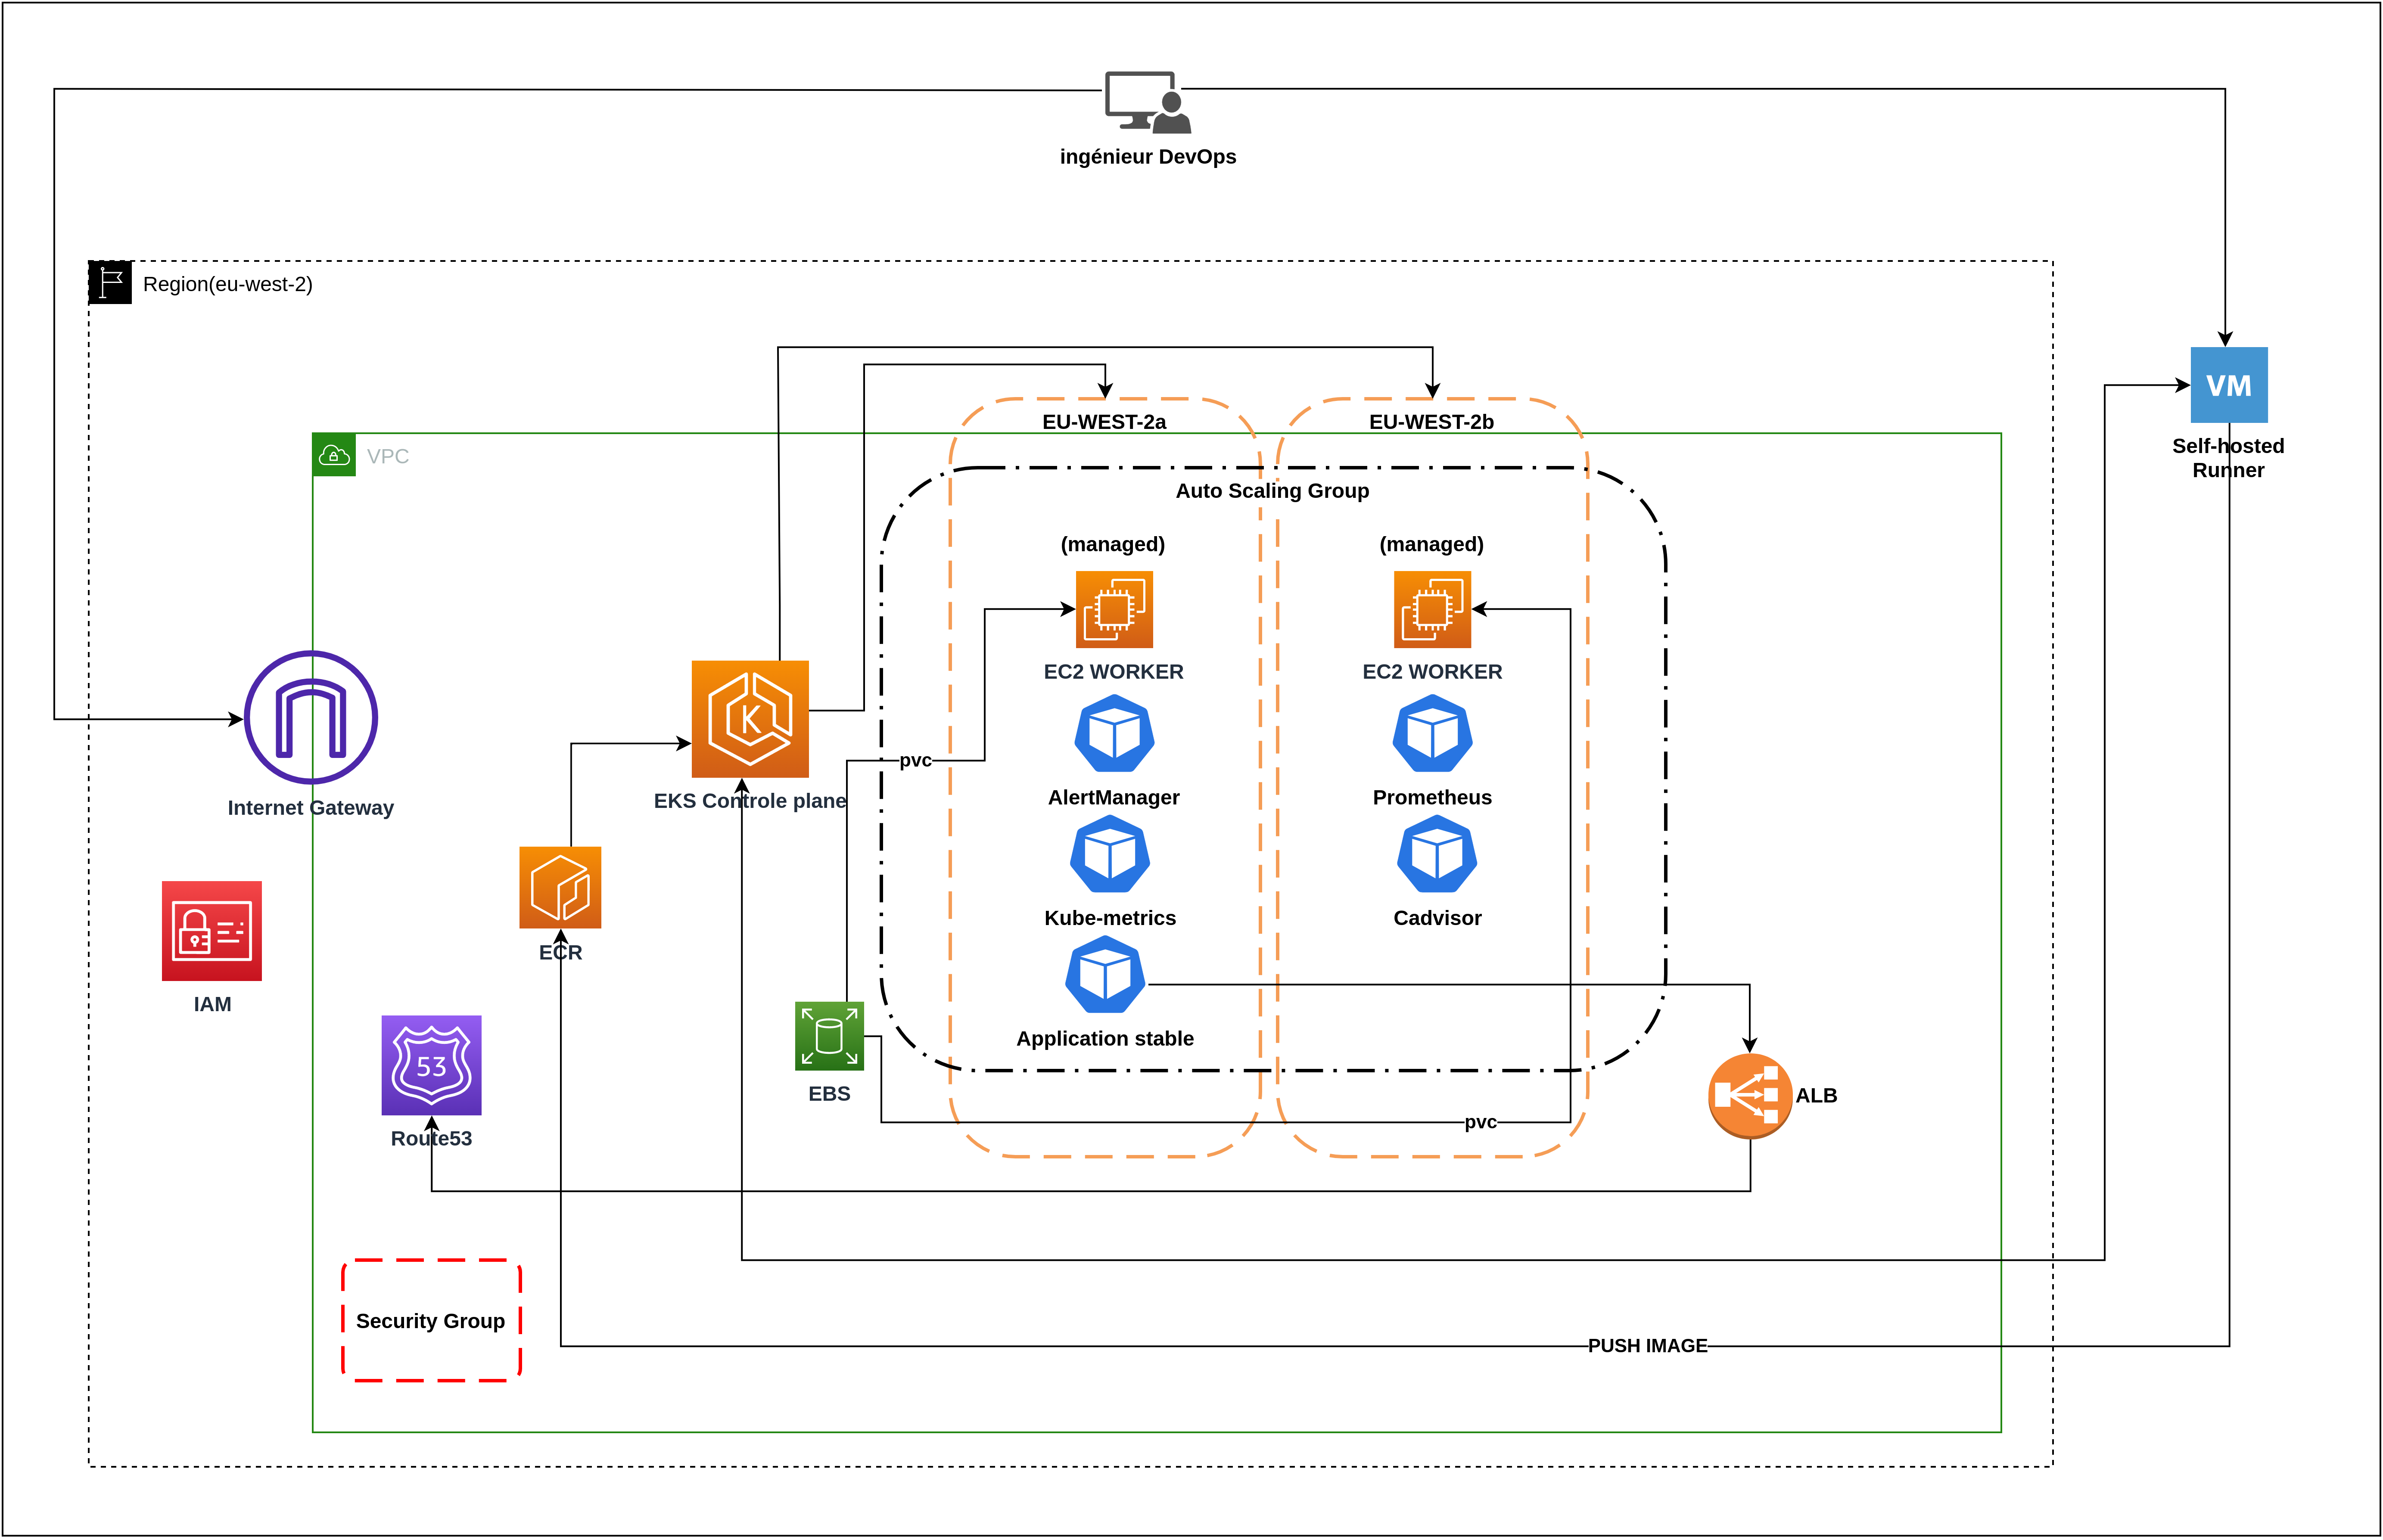
\includegraphics[width=18cm,height=14cm]{PARTIEEKS.drawio.png}
  
    \caption{Partie AWS}
  \end{figure}
  \indent
  \begin{tikzpicture}
   \draw[fill=black] (2,2) circle (2pt);
 \end{tikzpicture}
 Le cluster EKS se compose de nœuds de travail, qui sont des instances EC2 qui exécutent les conteneurs contenant la charge de travail de l’application. L’ingénieur de devops assure l’approvisionnement et la mise à l’échelle appropriés des nœuds de travailleurs en fonction des exigences de l’application et de la charge de travail. Cela implique de configurer des politiques de mise à l’échelle automatique pour ajuster automatiquement le nombre de nœuds de travail afin de gérer efficacement les différents charges de travail.
 \\[0.01cm]
 \indent
 \begin{tikzpicture}
  \draw[fill=black] (2,2) circle (2pt);
\end{tikzpicture}
Pour gérer le trafic entrant et le distribuer à travers les conteneurs du cluster EKS, un Load balancer est lancer pour aider à atteindre une haute disponibilité et une tolérance aux pannes en transférer les demandes vers les conteneurs, assurant ainsi une performance et une fiabilité optimales de l’application.
\\[0.01cm]
\indent
\begin{tikzpicture}
 \draw[fill=black] (2,2) circle (2pt);
\end{tikzpicture}  
Lorsque la branche EKS est déclenchée par des développeurs  leur code source, un pipeline dédié est lancé. Pour exécuter les actions de déploiement nécessaires sur le cluster EKS, un exécuteur configuré par l’ingénieur devops utilise son contexte et ses autorisations pour interagir efficacement avec le cluster. Cela permet un déploiement continu de l’application dans l’environnement de production hébergé sur le cluster EKS.
\\[0.01cm]
\indent
\begin{tikzpicture}
 \draw[fill=black] (2,2) circle (2pt);
\end{tikzpicture}  
Le surveillance du cluster EKS est également une responsabilité de l’ingénieur de devops. Prometheus installer sur EKS, fournissent des informations complètes sur les performances, l’utilisation des ressources et les paramètres de santé du cluster. Ce outil permettant à l’ingénieur de détecter et de résoudre rapidement les problèmes potentiels, assurant le bon fonctionnement de l’environnement de production.\\[0.3cm]
          
\textbf{\huge Conclusion}\\[0.5cm] 

Dans ce chapitre nous avons décrit les différents besoins fonctionnels et non fonctionnels. Aussi, nous avons décrit les diffèrents acteurs de système.Puis nous avons présentée les "User stories" en forme d'un product backlog.Par la suite, nous avons illustrée les cas d'utilisation avec des diagrammes. Puis, nous avons décrit les différents diagrammes de conception. Aussi, nous avons décrit la méthodologie de conception utiliser dans notre projet.Enfin, nous aussi présenter l'architecture global qui expliquer la fonctionnement du projet. Dans le chapitre suivante nous passerons à la phase de réalisation du projet.




\chapter{\Large Réalisation}

\textbf{\huge Introduction} \\[1cm]
\textsf{\fontfamily{ptm}\selectfont\scalefont{1.3}
Au cours de ce dernier chapitre, on va exposer le travail accompli, explorer les différent étapes pour realise le travail final en détaillons chaque étape et en incluant quelques captures d'écran expliquant le processus de déploiement de la solution.}\\[0.1cm]
\section{\fontfamily{ptm}\selectfont\Large  Environnement de travail }
\textsf{\fontfamily{ptm}\selectfont\scalefont{1.3}Dans cette partie, nous présentons les environnements matériels et logiciels utilisés dans le
cadre de notre projet.}
\subsection{\fontfamily{ptm}\selectfont\Large  Environnement matériel }
\textsf{\fontfamily{ptm}\selectfont\scalefont{1.3}Au cours de les différentes étape de notre projet, nous avons disposé de deux PC ayant les
caractéristiques figurantes dans le tableau ci-dessous :}
\begin{center}
    \begin{table}[H]  
      \centering
      \resizebox{1\textwidth}{!}{
  \begin{tabular}{|c|c|c|}
  \hline
    \textbf{Marque} &  \textbf{lenovo ideapad 3} & \textbf{Lenovo Legion slim 7} \\
  \hline
  \textbf{Processeur} & \textbf{AMD Rayzen 5 3.3GHZ} & \textbf{AMD Rayzen 9 4.10GHZ} \\
  \hline
  \textbf{Mémoire Vive} & \textbf{16GB RAM} & \textbf{16GB RAM} \\
  \hline
  \textbf{Stockage}& \textbf{500GB} & \textbf{1To}  \\
  \hline
  \textbf{Systéme d'exploitation }& \textbf{Fedora 37} &\textbf{Windows 11}\\
  \hline
  \end{tabular}
  }
  \caption{Caractéristiques des ordinateurs}
  \end{table}
  \end{center}
  \subsection{\fontfamily{ptm}\selectfont\Large  Environnement Logiciel }
  \textsf{\fontfamily{ptm}\selectfont\scalefont{1.3}Dans cette partie, nous présentons les environnements logiciels différents utilisés.(voir tableau 5.2)}
  \subsubsection{\fontfamily{ptm}\selectfont\Large  Environnement et technologie de développement }
  \newcolumntype{C}[1]{>{\centering\arraybackslash}p{#1}}
  \begin{center}
    \begin{table}[H]  
      \centering
      %\resizebox{0.8\textwidth}{!}{
  \begin{tabular}{|m{5cm}|m{5cm}|m{5cm}|}
  \hline
    \textbf{Nom} &  \textbf{Description} & \textbf{Utilisation} \\
  \hline
  \centering
\includegraphics[width=3cm,height=3cm]{autre_partie/VSCODE.png}   & \textbf{Visual Studio Code est un éditeur de code source développé par Microsoft.} & \textbf{Nous avons utilisé Visual studio code pour la développement de code et interagi avec github.} \\
  \hline
\centering
\includegraphics[width=2cm,valign=c]{autre_partie/VMW.png}&\textbf{VMware Workstation est un outil de virtualisation de poste de travail créé par la société VMware, il peut être utilisé pour mettre en place un environnement de test pour développer de nouveaux logiciels, ou pour tester l'architecture complexe d’un système d’exploitation avant de l’installer réellement sur une machine physique.\cite{21} }& \textbf{Nous avons utilisé Vmware pour créer diffèrent virtual machine pour deployée le cluster.} \\
\hline
\centering
\includegraphics[width=4cm,valign=c]{autre_partie/Latex.png}&\textbf{Latex est un logiciel de préparation de documents qui utilise le programme de composition TeX pour formater sa sortie, et est lui-même écrit dans le langage de macro TeX. Le latex est largement utilisé dans les universités pour la publication de documents scientifiques dans de nombreux domaines, y compris les mathématiques, l’informatique, etc.}& \textbf{Nous avons utilisé Latex pour rédaction de notre rapport.} \\
  \hline
  \centering
\includegraphics[width=2cm,valign=c]{autre_partie/GitHub-Logo.png}& \textbf{Github est un site développé par Chris Wanstrath, PJ Hyett et Tom Preston-Werner. Fournir divers services qui aident les développeurs à gérer leur code source à l'aide du logiciel de gestion de versions Git.} & \textbf{Nous avons utilisé Github pour déposer notre code.}  \\
  \hline
  \centering
\includegraphics[width=2cm,valign=c]{autre_partie/Docker-Symbol.png}& \textbf{Docker est une plate-forme qui rend l’exécution, le test et la livraison de logiciels plus rapide avec sa virtualisation au niveau OS qui permet de séparer l’application dans des conteneurs.} &\textbf{Nous avons utilisé docker dans la création des images docker.}\\
  \hline

  \end{tabular}
  %}
  \end{table}
  \end{center}
  \newpage
  \begin{center}
    \begin{table}[H]  
      \centering
      %\resizebox{0.8\textwidth}{!}{
  \begin{tabular}{|m{5cm}|m{5cm}|m{5cm}|}
  \hline
  \centering
\includegraphics[width=3cm,valign=c]{autre_partie/github-actions.png}& \textbf{GitHub Actions est une plateforme CI/CD (Continuous Integration and Continuous Delivery) qui vous permet d'automatiser votre pipeline de construction, de test et de déploiement. Vous pouvez créer des flux de travail qui construisent et testent chaque requête merge ,pull ou push sur votre dépôt.} & \textbf{Nous avons utilisé Github Action  pour la création et l'exécution de notre pipeline.}  \\
  \hline
  \centering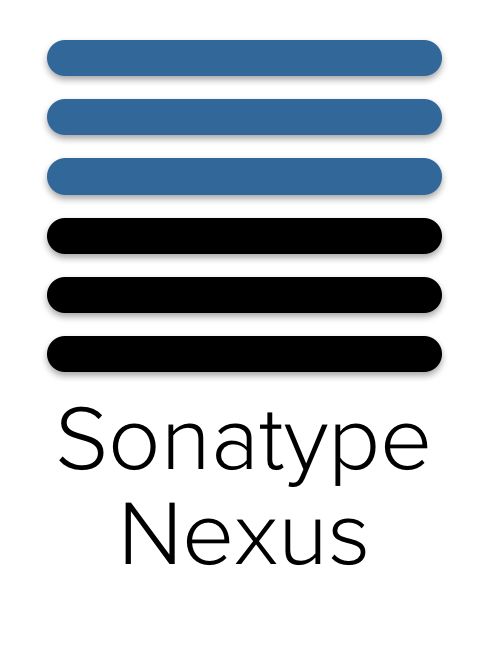
\includegraphics[width=3cm,valign=c]{autre_partie/Nexus.png}& \textbf{Nexus est gestionnaire de dépôt qui vous permet de proxy, collecter et gérer différents artefacts et image docker et rendre facile de distribuer votre logiciel. } & \textbf{Nous avons utilisé Nexus pour gérer notre artefact de l'application développer.}  \\
  \hline
  \centering
\includegraphics[width=3cm,valign=c]{autre_partie/SONARQ.png}& \textbf{sonarqube est une plateforme open source développée par SonarSource pour le contrôle de code qualité et les rapports de code statique, elle supporte différents langages et frameworks de programmation. } & \textbf{Nous avons utilisé Sonarqube pour l'analyse de notre code source et vérifier la présence des défauts.}  \\
  \hline
  \centering
\includegraphics[width=3cm,valign=c]{autre_partie/ANSIBLE.png}& \textbf{Ansible est un outil d’automatisation qui fournit une infrastructure en tant que code créé par Michael DeHaan et acquit par Red Hat, il fournit des outils pour la configuration, le déploiement d’application et le provisionnement. } & \textbf{Nous avons utilisé Ansible pour automatiser la configuration de cluster local et les ressources cloud.}  \\
  \hline
\centering
\includegraphics[width=4cm,valign=c]{autre_partie/K8s.png}& \textbf{Kubernetes est un système open source qui automatiser le déploiement, la mise à l’échelle et la gestion des applications dans des conteneurs} & \textbf{Nous avons utilisé Kubernetes pour la déploiement des diffèrent application et outils.}  \\
\hline
\centering
\includegraphics[width=3cm,valign=c]{autre_partie/prometheus-logo-png-transparent.png}& \textbf{Prometheus est un système open source développé par soundcloud pour la collection de données et de métriques à l’aide d’un modèle http pull. } & \textbf{Nous avons utilisé Prometheus pour la collection des diffèrent données des outils,clusters et applications.}  \\
\hline
\centering
\includegraphics[width=2cm,valign=c]{autre_partie/grafana-logo.png}& \textbf{Grafana est une application Web d’analyse open source et visualisation interactive. Il fournit des graphiques et des alertes lorsqu’il est connecté à des sources de données prises en charge. } & \textbf{Nous avons utilisé Grafana pour la création des alerts et visualisation des diffèrent données collecter par prometheus en forme des différent diagrammes.}  \\
\hline

  \end{tabular}
  %}
  \end{table}
  \end{center}
  \begin{center}
    \begin{table}[H]  
      \centering
      %\resizebox{0.8\textwidth}{!}{
  \begin{tabular}{|m{5cm}|m{5cm}|m{5cm}|}
  \hline
\centering
\includegraphics[width=4cm,valign=c]{autre_partie/Slack_RGB.png}& \textbf{Slack est un logiciel de messagerie développé par Slack Technologies.Slack est développé pour les communications professionnelles et organisationnelles. } & \textbf{Nous avons utilisé Slack pour recevoir les alert créer par Grafana.}  \\
\hline
\centering
\includegraphics[width=4cm,valign=c]{autre_partie/EKS.png}& \textbf{EKS is a service to create a managed kubernetes cluster by amazon it offers different add-ons that help to interact with other services like EBS,ALB or NLB. } & \textbf{Nous avons utilisé EKS pour créer un cluster pour l'environnement de production.}  \\
\hline
\centering
\includegraphics[width=3cm,valign=c]{autre_partie/ECR.png}& \textbf{Amazon elastic container Registry (Amazon ECR) est un service qui registre les images docker dans des répertoires soit public soit privé. } & \textbf{Nous avons utilisé ECR pour enregistrer notre diffèrent image docker.}  \\
\hline
\centering
\includegraphics[width=4cm,valign=c]{autre_partie/EC2.png}& \textbf{EC2 (Elastic Compute Cloud) est un serivce fourni par amazon faire facile aux utilisateurs de louer des ordinateurs virtuels pour exécuter leurs propres applications. } & \textbf{Nous avons utilisé EC2 pour créer des noued pour le cluster EKS.}  \\
\hline
\end{tabular}
%}
\caption{Environnement et technologies de développement}
\end{table}
\end{center}
  \subsection{\fontfamily{ptm}\selectfont\Large  Langage Informatique }
  \textsf{\fontfamily{ptm}\selectfont\scalefont{1.3} Le tableau ci-dessous répresente les diffèrents langage utilisé dans le projet.}  
  \newcolumntype{C}[1]{>{\centering\arraybackslash}p{#1}}
  \begin{center}
    \begin{table}[H]  
      \centering
      %\resizebox{0.8\textwidth}{!}{
  \begin{tabular}{|m{5cm}|m{5cm}|m{5cm}|}
  \hline
    \textbf{Nom} &  \textbf{Description} & \textbf{Utilisation} \\
  \hline
\centering
\includegraphics[height=2cm,width=2cm]{autre_partie/ReactJs.png}   & \textbf{React js est une bibliothèque open source utilisée pour construire des interfaces, il peut également être utilisé sur IOS, Android et web } & \textbf{Cette langage est utilisée dans l'application qui nous avons testé dans notre projet.} \\
  \hline
  \centering\includegraphics[width=2cm,valign=c]{autre_partie/yaml.png}&\textbf{YAML (Ain’t Markup Language) un langage de sérialisation de données développé par Clark Evans, Ingy döt Net et Oren Ben-Kiki, utilisé pour créer des fichiers de configuration.}& \textbf{Nous avons utilisé ce langage pour créer différent playbooks. } \\
  \hline
\end{tabular}
%}
\caption{Langage informatique}
\end{table}
\end{center}
\subsection{\fontfamily{ptm}\selectfont\Large  Environnement de Conception}
\textsf{\fontfamily{ptm}\selectfont\scalefont{1.3} Le tableau ci-dessous répresente les diffèrents outil de conception utilisé dans le projet.}  
\newcolumntype{C}[1]{>{\centering\arraybackslash}p{#1}}
\begin{center}
  \begin{table}[H]  
    \centering
    %\resizebox{0.8\textwidth}{!}{
\begin{tabular}{|m{5cm}|m{5cm}|m{5cm}|}
\hline
  \textbf{Nom} &  \textbf{Description} & \textbf{Utilisation} \\
\hline
\centering\includegraphics[width=2cm,valign=c]{autre_partie/Draw.png}   & \textbf{draw.io est une application de source libre qu'il est utiliser pour illustrer des diagrammes. } & \textbf{Ce outil est utilisée pour les différents diagrammes dans notre projet.} \\
\hline
\centering\includegraphics[width=4cm,valign=c]{autre_partie/Canva-Logo.png}&\textbf{Canva est un outil de conception graphique en ligne gratuit,utiliser pour créer des présentations, des logos et plus encore}& \textbf{Nous avons utilisé canva pour désigner quelque diagrammes. } \\
\hline
\end{tabular}
%}
\caption{Environnement de conception}
\end{table}
\end{center}
\section{\fontfamily{ptm}\selectfont\Large Sprint1 :Configuration de l'architecture cloud}
\textsf{\fontfamily{ptm}\selectfont\scalefont{1.3} Pour ce partie nous allons configuré tout les ressources cloud que nous besoin pour la projet.}
\subsection{\fontfamily{ptm}\selectfont\Large  Configuration des ressources cloud}
\textsf{\fontfamily{ptm}\selectfont\scalefont{1.3} Pour la configuration des ressources cloud nous avons préparer un playbook ansible qui créer les ressources nécessaire dans AWS comme VPC,Subnets,route,security groups,EKS and ECR.ou début en definit les différent variables pour les ressources}
\begin{figure}[H]
    \begin{center}
    \fbox{\includegraphics[height=10cm,width=10cm]{autre_partie/VARS.png}}
    \end{center}
    \caption{Les variables de playbook ansible}
    \end{figure}
    \textsf{\fontfamily{ptm}\selectfont\scalefont{1.3}Aprés la définition des variable dans le playbook on passe a les tâches qui sera exécuter par Ansible:\\
    \indent
     \begin{tikzpicture}
        \draw[fill=black] (2,2) circle (2pt);
      \end{tikzpicture} Tâche << Créer VPC >>:
      \begin{figure}[H]
        \begin{center}
        \fbox{\includegraphics[width=10cm]{VPC.png}}
        \end{center}
        \caption{Tâche de VPC} 
        \end{figure}
        \indent
        \begin{tikzpicture}
           \draw[fill=black] (2,2) circle (2pt);
         \end{tikzpicture} Tâche << Créer les sous-réseaux >>:
         \begin{figure}[H]
           \begin{center}
           \fbox{\includegraphics[width=10cm]{SUBNETS.png}}
           \end{center}
           \caption{Tâche des sous-réseaux}
           \end{figure}
           \indent
           \begin{tikzpicture}
              \draw[fill=black] (2,2) circle (2pt);
            \end{tikzpicture} Tâche << Créer passerelle Internet >>:
            \begin{figure}[H]
              \begin{center}
              \fbox{\includegraphics[width=11cm]{IGW.png}}
              \end{center}
              \caption{Tâche de passerelle internet}
              \end{figure}
              \indent
              \begin{tikzpicture}
                 \draw[fill=black] (2,2) circle (2pt);
               \end{tikzpicture} Tâche << Créer route >>:
               \begin{figure}[H]
                 \begin{center}
                 \fbox{\includegraphics[width=11cm]{ROUTE.png}}
                 \end{center}
                 \caption{Tâche de route internet}
                \end{figure}
                \indent
                \begin{tikzpicture}
                   \draw[fill=black] (2,2) circle (2pt);
                 \end{tikzpicture} Tâche << Créer la sécurite groupe >>:
                 \begin{figure}[H]
                   \begin{center}
                   \fbox{\includegraphics[width=11cm]{SECURITYGR.png}}
                   \end{center}
                   \caption{Tâche de sécurité groupe.}
                  \end{figure}
                  \indent
                  \begin{tikzpicture}
                     \draw[fill=black] (2,2) circle (2pt);
                   \end{tikzpicture} Tâche << Créer EKS cluster >>:
                   \begin{figure}[H]
                     \begin{center}
                     \fbox{\includegraphics[width=11cm]{EKSCL.png}}
                     \end{center}
                     \caption{Tâche de cluster EKS.}
                    \end{figure}
                    \indent
                    \begin{tikzpicture}
                       \draw[fill=black] (2,2) circle (2pt);
                     \end{tikzpicture} Tâche << Créer Noeud de travail pour le cluster EKS >>:
                     \begin{figure}[H]
                       \begin{center}
                        \fbox{ \includegraphics[width=11cm]{WORKERNODES.png}}
                       \end{center}
                       \caption{Tâche de noeud de travail.}
                      \end{figure}
                      \indent
                      \begin{tikzpicture}
                         \draw[fill=black] (2,2) circle (2pt);
                       \end{tikzpicture} Tâche << Créer répertoire ECR >>:
                       \begin{figure}[H]
                         \begin{center}
                            \fbox{\includegraphics[width=11cm]{ECRPH.png}}
                         \end{center}
                         \caption{Tâche de ECR}
                        \end{figure}
                        \indent
                        \begin{tikzpicture}
                           \draw[fill=black] (2,2) circle (2pt);
                         \end{tikzpicture} Résultat de l'execution de playbook (voir figure 5.10):
                         \begin{figure}[H]
                           \begin{center}
                              \fbox{\includegraphics[width=17cm,height=13cm]{EKSRESPUP.png}}
                           \end{center}
                           \caption{Résultat de playbook.}
                          \end{figure}
                          }   
%%%%%%%%%%%%%%%%%%%%%%%%%%%%%%%%%%%%%%%%%%%ADDDDDDDDDDDDDDDDDDDDD_RESULTATSSSSSSSSSSSSSSSSSSSSSSSSSSSSS%%%%%%%%%%%%%%%%%%%%%%%%%%%%%%%%%%%%%%%
\subsection{\fontfamily{ptm}\selectfont\Large  Configuration de cluster local}
\textsf{\fontfamily{ptm}\selectfont\scalefont{1.3} Pour ce partie nous allons configuré tout les ressources local que nous besoin pour la projet.}
\subsubsection{\fontfamily{ptm}\selectfont\Large  Provisionnement de les machines virtuelles}
\textsf{\fontfamily{ptm}\selectfont\scalefont{1.3} Nous allons configuré les machines virtuelles pour enfin installer le cluster local et déployé les outils nécessaire pour la fonctionnement de projet.\\
\begin{tikzpicture} 
    \draw[fill=black] (2,2) circle (2pt);
  \end{tikzpicture} La création des virtuelles machines sera faite avec Vmware Workstation (voir figure 5.11)
  \begin{figure}[H]
    \begin{center}
       \fbox{\includegraphics[width=18cm]{VM.png}}
    \end{center}
    \caption{Les machines virtuelles.}
   \end{figure}
Pour la configuration de cluster nous avons utilisé Ansible pour l'optimisation du temps:\\
\begin{tikzpicture} 
    \draw[fill=black] (2,2) circle (2pt);
  \end{tikzpicture} L'installation des logiciels nécessaire sera fait avec ansible on exécutent le playbook "Configuration.yaml" sur les machines virtuelles.(voir figure 5.12, 5.13 et 5.14)
  \begin{figure}[H]
    \begin{center}
       \fbox{\includegraphics[width=17cm,height=13cm]{installer.png}}
    \end{center}
    \caption{Playbook Ansible d'installation(1).}
   \end{figure}
   \begin{figure}[H]
    \begin{center}
       \fbox{\includegraphics[width=10cm,height=15cm]{installer2.png}}
    \end{center}
    \caption{Playbook Ansible d'installation(2).}
   \end{figure}
   \begin{figure}[H]
    \begin{center}
       \fbox{\includegraphics[width=10cm,height=15cm]{installer3.png}}
    \end{center}
    \caption{Playbook Ansible d'installation(3).}
   \end{figure}
   \indent\indent Le résultat de l'exécution de ce playbook aprés le commande "ansible-playbook Configuration.yaml"(voir figure 5.15)
   \begin{figure}[H]
    \begin{center}
       \fbox{\includegraphics[width=17cm,height=9cm]{resultatwhit.png}}
    \end{center}
    \caption{résultat d'installation.}
   \end{figure}
   \begin{tikzpicture} 
    \draw[fill=black] (2,2) circle (2pt);
  \end{tikzpicture} Aprés l'installation, la configuration de la machine master sera fait avec playbook "ConfigMaster.yaml"(voir figure 5.156
   \begin{figure}[H]
    \begin{center}
       \fbox{\includegraphics[width=10cm,height=13cm]{Conf.png}}
    \end{center}
    \caption{playbook Configuration de master.}
   \end{figure}
    \indent\indent Résultats de l'exécution de la playbook "ConfigMaster.yaml" (voir figure 5.17)
    \begin{figure}[H]
        \begin{center}
           \fbox{\includegraphics[width=17cm,height=12cm]{CONF.png}}
        \end{center}
        \caption{Résultat de playbook "ConfigurationMaster.yaml".}
       \end{figure} 
       \begin{tikzpicture} 
        \draw[fill=black] (2,2) circle (2pt);
      \end{tikzpicture} Le cluster requis une configuration de réseau pour la communication entre les noeuds et les pods pour configurer le réseau nous avons préparer un playbook "NetworkPolicy.yaml" (voir figure 5.18)
       \begin{figure}[H]
        \begin{center}
           \fbox{\includegraphics[width=18cm,height=9cm]{Network.png}}
        \end{center}
        \caption{playbook NetworkPolicy.yaml.}
       \end{figure}
       \indent\indent Résultats de l'exécution de la playbook "NetworkPolicy.yaml" (voir figure 5.19)
       \begin{figure}[H]
           \begin{center}
              \fbox{\includegraphics[width=18cm,height=12cm]{NetworkWHITE.png}}
           \end{center}
           \caption{Résultat de playbook "NetworkPolicy.yaml".}
          \end{figure} 
          \begin{tikzpicture} 
            \draw[fill=black] (2,2) circle (2pt);
        \end{tikzpicture} Aprés la configuration de calico dans le cluster l'ingénieur DevOps exécute la commande "Kubeadm join" qui est afficher aprés l'exécution de playbook "NetworkPolicy.yaml", dans les noeud qui nous avons créé comme des noeuds du travail.(voir figure 5.19 pour le commande "Kubeadm join").\\Enfin la cluster local est prét(voir figure 5.20)
        \begin{figure}[H]
         \begin{center}
            \fbox{\includegraphics[width=15cm,height=10cm]{CLUSTERLOCAL.png}}
         \end{center}
         \caption{Cluster locale.}
        \end{figure}
         }
         \subsubsection{\fontfamily{ptm}\selectfont\Large  Configuration de Sonarqube}
         \textsf{\fontfamily{ptm}\selectfont\scalefont{1.3} Nous allons configuré et déployé SonarQube sur notre cluster pour analyse la qualité de notre code .\\
         \begin{tikzpicture} 
             \draw[fill=black] (2,2) circle (2pt);
           \end{tikzpicture} Pour déployé SonarQube il faut créer les diffèrent fichier nécessaire (voir figure 5.21)
           \begin{figure}[H]
             \begin{center}
                \fbox{\includegraphics[width=8cm]{SONARFILES.png}}
             \end{center}
             \caption{Liste des fichier (SonarQube).}
            \end{figure}
            \indent\indent Ces fichier sont déployé aprés l'exécution de commande:\\\indent\indent "kubectl apply -f ./sonarqube -n sonarqube" (voir figure 5.22)
            \begin{figure}[H]
                \begin{center}
                   \fbox{\includegraphics[width=14cm]{SONAKUBE.png}}
                \end{center}
                \caption{Pod SonarQube.}
               \end{figure}      
               \indent\indent La figure suivante présente l'interface de SonarQube (voir figure 5.23)
               \begin{figure}[H]
                   \begin{center}
                      \fbox{\includegraphics[width=18cm]{SONARINTERFACE.png}}
                   \end{center}
                   \caption{Interface de SonarQube.}
                  \end{figure}             
         }
         \subsubsection{\fontfamily{ptm}\selectfont\Large  Configuration de Nexus}
         \textsf{\fontfamily{ptm}\selectfont\scalefont{1.3} Nous allons configuré et déployé Nexus sur notre cluster stocker les artefacts de notre code.\\
         \begin{tikzpicture} 
             \draw[fill=black] (2,2) circle (2pt);
           \end{tikzpicture} Pour déployé Nexus il faut créer les diffèrent fichier nécessaire (voir figure 5.24)
           \begin{figure}[H]
             \begin{center}
                \fbox{\includegraphics[width=7cm]{NEXUSFILES.png}}
             \end{center}
             \caption{Liste des fichier (Nexus).}
            \end{figure}
            \indent\indent Ces fichier sont déployé aprés l'exécution de commande:\\\indent\indent "kubectl apply -f ./nexus -n nexus" (voir figure 5.25)
            \begin{figure}[H]
                \begin{center}
                   \fbox{\includegraphics[width=14cm]{NEXUSKUBE.png}}
                \end{center}
                \caption{Pod Nexus.}
               \end{figure} 
               \indent\indent La figure suivante présente l'interface de Nexus (voir figure 5.26):
               \begin{figure}[H]
                   \begin{center}
                      \fbox{\includegraphics[width=18cm]{NEXUSINTERFACE.png}}
                   \end{center}
                   \caption{Interface de Nexus.}
                  \end{figure} 
         }
         \subsubsection{\fontfamily{ptm}\selectfont\Large  Outils des surveillances}
         \textsf{\fontfamily{ptm}\selectfont\scalefont{1.3}\\
         \begin{tikzpicture} 
             \draw[fill=black] (2,2) circle (2pt);
           \end{tikzpicture} Pour déployé les outils des surveillances il faut créer les diffèrent fichier nécessaire (voir figure 5.27)
           \begin{figure}[H]
             \begin{center}
                \fbox{\includegraphics[width=7cm]{MONITORING.png}}
             \end{center}
             \caption{Liste des fichier (Monitoring).}
            \end{figure}
            \indent\indent Ces fichier sont déployé aprés l'exécution de commande:\\\indent\indent "kubectl apply -f ./Monitoring -n monitoring"(voir figure 5.28)
            \begin{figure}[H]
                \begin{center}
                   \fbox{\includegraphics[width=15cm]{MONIKUBE.png}}
                \end{center}
                \caption{Les Pods de namespace Monitoring.}
               \end{figure} error: unable to upgrade connection: container not found ("grafana")
                }
\section{\fontfamily{ptm}\selectfont\Large Sprint2 :Configuration de pipeline}
\textsf{\fontfamily{ptm}\selectfont\scalefont{1.3} Pour ce partie nous allons configuré les workflow qui sont lancer quand une changement dans notre code est détecter.}
\subsection{\fontfamily{ptm}\selectfont\Large  Création des pipelines}
\textsf{\fontfamily{ptm}\selectfont\scalefont{1.3} Configuration de pipeline pour les différent branches:\\
\begin{tikzpicture} 
    \draw[fill=black] (2,2) circle (2pt);
  \end{tikzpicture} Pipeline de branche Main (voir figure 5.29 et 5.30)
  \begin{figure}[H]
    \begin{center}
       \fbox{\includegraphics[width=17cm,height=12cm]{PIPE111.png}}   
    \end{center}
    \caption{Pipeline de branche main(1).}
   \end{figure}
     \begin{figure}[H]
    \begin{center}
       \fbox{\includegraphics[width=17cm,height=12cm]{PIPE121.png}}
    \end{center}
    \caption{Pipeline de branche main(2).}
   \end{figure}
   \indent\indent Encore de la lancement de la pipeline différent action sera exécuter (voir figure 5.31)
   \begin{figure}[H]
       \begin{center}
          \fbox{\includegraphics[width=10cm,height=12cm]{GITA1.png}}
       \end{center}
       \caption{Github Action interface.}
      \end{figure}
      \begin{tikzpicture} 
        \draw[fill=black] (2,2) circle (2pt);
      \end{tikzpicture} Pipeline de branche EKS (voir figure 5.32 et 5.33)
      \begin{figure}[H]
        \begin{center}
           \fbox{\includegraphics[width=18.5cm,height=13cm]{PIPE211.png}}   
        \end{center}
        \caption{Pipeline de branche EKS(1).}
       \end{figure}
         \begin{figure}[H]
        \begin{center}
           \fbox{\includegraphics[width=18cm,height=9cm]{PIPE222.png}}
        \end{center}
        \caption{Pipeline de branche EKS(2).}
       \end{figure}
       \indent\indent Encore de la lancement de la pipeline différent action sera exécuter (voir figure 5.34)
       \begin{figure}[H]
           \begin{center}
              \fbox{\includegraphics[width=10cm,height=12cm]{GITA2.png}}
           \end{center}
           \caption{Github Action interface.}
          \end{figure}
}
\subsection{\fontfamily{ptm}\selectfont\Large  Configuration d'exécuteur local }
\textsf{\fontfamily{ptm}\selectfont\scalefont{1.3} Pour ce partie nous allons configuré l'exécuteur qui exécuter les workflows de notre projet.(voir figure 5.35)}
\begin{figure}[H]
    \begin{center}
       \fbox{\includegraphics[width=18cm]{RUNNER.png}}
    \end{center}
    \caption{Github Action Runner.}
   \end{figure}
   \textsf{\fontfamily{ptm}\selectfont\scalefont{1.3} Aprés l'exécution d'un pipeline l'application sera deployé dans l'environnement corespond a la besoin.\\
   \begin{tikzpicture} 
      \draw[fill=black] (2,2) circle (2pt);
    \end{tikzpicture} Le figure suivante présente l'application exécuter par le pipline dans l'environnement test (voir figure 5.36) :
  \begin{figure}[H]
      \begin{center}
         \fbox{\includegraphics[width=17cm,height=8cm]{APPTEST.png}}
      \end{center}
      \caption{Application dans environnement test.}
     \end{figure}
     L'image docker de cette version d'application sera stocker dans ECR (voir figure 5.37)
     \begin{figure}[H]
      \begin{center}
         \fbox{\includegraphics[width=17cm,height=6cm]{ECRREPO1.png}}
      \end{center}
      \caption{Répertoire des images ECR.}
     \end{figure}
     \begin{tikzpicture} 
      \draw[fill=black] (2,2) circle (2pt);
    \end{tikzpicture} Le figure suivante présente l'application exécuter par le pipline dans l'environnement prod:
  \begin{figure}[H]
      \begin{center}
         \fbox{\includegraphics[width=17cm,height=8cm]{APPFINAL.png}}
      \end{center}
      \caption{Application dans environnement production.}
     \end{figure}
     L'image docker de cette version d'application sera stocker dans ECR (voir figure)
     \begin{figure}[H]
      \begin{center}
         \fbox{\includegraphics[width=17cm,height=6cm]{ECRREPO2.png}}
      \end{center}
      \caption{Image latest dans ECR.}
     \end{figure}
   }
\section{\fontfamily{ptm}\selectfont\Large Sprint3: Mise en place d'un systéme du monitoring}
\textsf{\fontfamily{ptm}\selectfont\scalefont{1.3}Nous avons configuré et déployé des surveillances pour collecter,analyse et stocker les données de notre cluster.\\
\subsection{\fontfamily{ptm}\selectfont\Large Configuration de Prometheus}
\begin{tikzpicture} 
    \draw[fill=black] (2,2) circle (2pt);
  \end{tikzpicture} Interface de Prometheus(voir figure 5.40)
\begin{figure}[H]
    \begin{center}
       \fbox{\includegraphics[width=17cm,height=8cm]{PROMETHEUSINTERFACE1.png}}
    \end{center}
    \caption{Interface Prometheus.}
   \end{figure}
   }
   \subsection{\fontfamily{ptm}\selectfont\Large Configuration de AlertManager}
   \textsf{\fontfamily{ptm}\selectfont\scalefont{1.3}
   \begin{tikzpicture} 
       \draw[fill=black] (2,2) circle (2pt);
     \end{tikzpicture} Interface de AlertManager(voir figure 5.41)
   \begin{figure}[H]
       \begin{center}
          \fbox{\includegraphics[width=18cm]{ALERTINTERFACE.png}}
       \end{center}
       \caption{Interface AlertManager.}
      \end{figure}
      \begin{tikzpicture} 
        \draw[fill=black] (2,2) circle (2pt);
      \end{tikzpicture} Nous avons configuré aussi Slack pour recevoir les notifications des alertes (voir figure 5.42)
    \begin{figure}[H]
        \begin{center}
           \fbox{\includegraphics[width=18cm]{SLACKALERT.png}}
        \end{center}
        \caption{Interface de Slack.}
       \end{figure}
}
\subsection{\fontfamily{ptm}\selectfont\Large Configuration des Dashboards Grafana}
\textsf{\fontfamily{ptm}\selectfont\scalefont{1.3} Nous avons configuré les diffèrent dashboards qui nous allons utilisé pour la visualisation des données et métriques collecter par prometheus.\\
\begin{tikzpicture} 
    \draw[fill=black] (2,2) circle (2pt);
  \end{tikzpicture} Interface de Grafana(voir figure 5.43)
\begin{figure}[H]
    \begin{center}
       \fbox{\includegraphics[width=17cm,height=10cm]{Grafana2.png}}
    \end{center}
    \caption{Interface Grafana.}
   \end{figure}
\indent\indent Dans les figures suivante nous allons présenté diffèrent exemple des Dashboard:\\
\begin{tikzpicture} 
    \draw[fill=black] (2,2) circle (2pt);
\end{tikzpicture} Exemple: dashboard de Local cluster(voir figure 5.44)
\begin{figure}[H]
    \begin{center}
       \fbox{\includegraphics[width=18.5cm,height=13cm]{EXEMPLE11.png}}
    \end{center}
    \caption{dashboard de Local cluster.}
   \end{figure}
   \begin{tikzpicture} 
    \draw[fill=black] (2,2) circle (2pt);
\end{tikzpicture} Exemple: dashboard de SonarQube(voir figure 5.45)
\begin{figure}[H]
    \begin{center}
       \fbox{\includegraphics[width=18.5cm,height=13cm]{EXEMPLE22.png}}
    \end{center}
    \caption{dashboard de SonarQube.}
   \end{figure}
   \begin{tikzpicture} 
    \draw[fill=black] (2,2) circle (2pt);
\end{tikzpicture} Exemple: dashboard de EKS cluster(voir figure 5.46)
\begin{figure}[H]
    \begin{center}
       \fbox{\includegraphics[width=18cm]{EXEMPLE31.png}}
    \end{center}
    \caption{dashboard de EKS cluster.}
   \end{figure}            
}
\section{\fontfamily{ptm}\selectfont\Large Conclusion}
 \textsf{\fontfamily{ptm}\selectfont\scalefont{1.3} Dans ce chapitre nous avons entamé la réalisation du projet tout en insistant sur quelques scénarios qui montrent les fonctionnalités majeures de l’application. 
}

\chapter{Sprint2:Configuration de la Pipline.}
\newpage
\textbf{\huge Introduction} \\[1cm]
\textsf{\fontfamily{qtm}\selectfont\scalefont{1.3}
Après avoir vue la configuration de l'architecture cloud aws nous présentent la deuxième sprint, nous commençons par l'objectif de sprint puis l'architecture globale ensuite nous détaillons le diagramme d'utilisation et séquence détaille, Finalement, nous allons exposer la partie réalisation.}


\section{\LARGE Objectif du Sprint}
\textsf{\fontfamily{qtm}\selectfont\scalefont{1.3}Ce sprint est à propos de configurer pipline  dont le but est d'améliorer l'efficacité et la qualité du développement logiciel, tout en minimisant les erreurs et les temps d'arrêt.}

\section{\LARGE Architecture Détaillée}
\textsf{\fontfamily{qtm}\selectfont\scalefont{1.3}Dans cette partie nous allons présenter l'architecture détaillée correspond au sprint.}

\subsection{\Large Diagramme Cas d'utilisation Détaillée}
\textsf{\fontfamily{qtm}\selectfont\scalefont{1.3}Pour éliminer toute ambiguïté et éclaircir le cas d'utilisation, nous présentons le cas en détail.}

\begin{figure}[H]
    \begin{center}
    \includegraphics[height=10cm]{configuration pipline use case.png}
    \end{center}
    \caption{cas d’utilisation"Configuration de la Pipline"}
    %\floatfoot{Source: (Citation command)}
    % avec le package "floatrow"
    \end{figure}

\textsf{\fontfamily{qtm}\selectfont\scalefont{1.3}
    Pour expliquer  le diagramme de cas d’utilisation, nous représentons la description textuelle du principales fonctionnalités mentionnées ci-dessus : \\}
    \begin{center}
       \begin{table}[H]  
         \centering
         \resizebox{1.1\textwidth}{!}{%
         \begin{tabular}{|c|p{13cm}|}
          \hline
          Titre & Configuration de la Pipline\\
          \hline
          Acteur & Ingénieur DevOps \\
          \hline
          Description & L'ingénieur DevOps gérait la configuration de la Pipline  et la création du cluster .\\
          \hline
          Pré conditions & Comprendre le processus de déploiement de l' application,
aussi disposer d'une infrastructure appropriée pour prendre en charge le déploiement ,
ainsi identifier les étapes du processus de déploiement, les dépendances et les outils nécessaires.
et pour  automatiser les étapes du pipeline en utilisant des scripts et des configurations. \\
          \hline
          Post conditions & une architecture configurait correctement.  \\
          \hline 
          Scénario nominal & Déploiement continu est réussite et la configuration réussite.\\
          \hline
          Scénario alternatif & problème de compatibilité avec l'infrastructure existante ou la configuration n'est pas correcte.  \\
          \hline
          \end{tabular}%
         }
       \caption{Description de cas d’utilisation}
       \end{table}
       \end{center}
       \subsection{\Large Diagramme de sequance  Détaillée}
       \textsf{\fontfamily{qtm}\selectfont\scalefont{1.3}
       Nous détaillons ci-dessous les interactions générales du système}
       \begin{figure}[H]
    \begin{center}
    \includegraphics[height=14cm,width=18cm]{sequencepipeline.drawio}
    \end{center}
    \caption{diagramme de séqunce"Configuration de la Pipline"}
    %\floatfoot{Source: (Citation command)}
    % avec le package "floatrow"
    \end{figure}

\chapter{Sprint3: Déploiement de l'application sur le cluster.}
\newpage
\textbf{\huge Introduction} \\[1cm]

\textsf{\fontfamily{qtm}\selectfont\scalefont{1.3}
Après avoir déduit la configuration du pipline nous présentent la troisieme  sprint, nous commençons par l'objectif de sprint puis l'architecture globale ensuite nous détaillons le diagramme d'utilisation et séquence détaille, Finalement, nous allons exposer la partie réalisation}


\section{\LARGE Objectif du Sprint}
\textsf{\fontfamily{qtm}\selectfont\scalefont{1.3} l'objectif du déploiement de l'application sur un cluster est d'assurer une disponibilité élevée, une évolutivité, une tolérance aux pannes, une gestion efficace des ressources, une sécurité, une facilité de déploiement et une surveillance pour fournir une expérience utilisateur optimale dans un environnement de cluster.}


\section{\LARGE Architecture Détaillée}
\textsf{\fontfamily{qtm}\selectfont\scalefont{1.3}Dans cette partie nous allons présenter l'architecture détaillée correspond au sprint.}

\subsection{\Large Diagramme Cas d'utilisation Détaillée}
\textsf{\fontfamily{qtm}\selectfont\scalefont{1.3}Afin d'éliminer toute ambiguïté et de clarifier le cas d'utilisation, nous présentons le cas de façon détaillée.}

\begin{figure}[H]
    \begin{center}
    \includegraphics[height=10cm]{usecasedet.drawio.png}
    \end{center}
    \caption{cas d’utilisation"Déploiement de l'application sur
le cluster."}
    %\floatfoot{Source: (Citation command)}
    % avec le package "floatrow"
    \end{figure}

  \textsf{\fontfamily{qtm}\selectfont\scalefont{1.3}
    Pour expliquer  le diagramme de cas d’utilisation, nous représentons la description textuelle du principales fonctionnalités mentionnées ci-dessus : \\}
    \begin{center}
       \begin{table}[H]  
         \centering
         \resizebox{1.1\textwidth}{!}{%
         \begin{tabular}{|c|p{13cm}|}
          \hline
          Titre & Déploiement de l'application sur
le cluster.\\
          \hline
          Acteur & Ingénieur DevOps \\
          \hline
          Description & L'ingénieur DevOps gérait transférer l'application et ses composants dans un environnement de cluster, dans lequel elle peut être exécutée et gérée de façon efficace et évolutive .\\
          \hline
          Pré conditions & La configuration de cluster ainsi la configuration de l'application et la gestion des depandances . \\
          \hline
          Post conditions & l'application deploye sur cluster et bien fonctionne .  \\
          \hline 
          Scénario nominal &  l'application est déployée avec succès sur le cluster, fonctionne de manière stable et répond aux exigences spécifiées.\\
          \hline
          Scénario alternatif & problèmes lors de la configuration du cluster ou  problèmes de configuration de l'application , de réseau ou de ressources insuffisantes.  \\
          \hline
          \end{tabular}%
         }
       \caption{Description de cas d’utilisation}
       \end{table}
       \end{center}

%\chapter{Résultats}

\section{Partie 1}

Intro

\subsection{Sous-partie 1}

\paragraph*{Paragraphe 1 (n'apparaitra pas dans l'index)} Bla

\paragraph*{Paragraphe 2} Bla

\paragraph*{Paragraphe 3} Bla

\subsection{Sous-partie 2}

Bla

\subsection{Sous-partie 3}

Bla

\section{Partie 2}

Intro

\subsection*{Sous-partie 1 ('apparaitra pas dans l'index)} Bla

\paragraph*{Paragraphe 1 ('apparaitra pas dans l'index)} Bla

\paragraph*{Paragraphe 2} Bla

\paragraph*{Paragraphe 3} Bla

\newpage

\subsection*{Sous-partie 2}

Bla

%galerie d'image
\begin{figure}[htp]
  \centering
  \subfloat[Première image]{\label{fig:première}\includegraphics[scale=0.8]{resultats/gallerie}}
  ~ %espace entre deux images sur une même ligne
  \subfloat[Deuxième image]{\label{fig:deuxième}\includegraphics[scale=0.8]{resultats/gallerie}}
  ~
  \subfloat[Troisième image]{\label{fig:troisième}\includegraphics[scale=0.8]{resultats/gallerie}}
  ~\\ %saute une ligne dans la galerie d'image
  \subfloat[Quatrième image]{\label{fig:quatrième}\includegraphics[scale=0.8]{resultats/gallerie}}
  ~
  \subfloat[Cinquième image]{\label{fig:cinquième}\includegraphics[scale=0.8]{resultats/gallerie}}
  \caption{Différents screenshots quelque chose, en gallerie}
  \label{fig:gallerie1}
\end{figure}

%\chapter{Bilan}

%Rappel du context
Intro / Rappel Contexte

Nous avons donc pu en tirer la problématique suivante :

\begin{center}
\hskip7mm
Problématique du sujet
\end{center}

Bla

Bla\\

Bla\\

%Rappel des résultats
Bla

Bla\\

Bla

Bla

\newpage

%Conclusion/Perspectives
Bla

Bla\\

Bla

%%Ne pas numéroter cette partie
\part*{Annexes}
%Rajouter la ligne "Annexes" dans le sommaire
\addcontentsline{toc}{part}{Annexes}

\chapter*{Annexe 1}
\addcontentsline{toc}{chapter}{Annexe 1}

%changer le format des sections, subsections pour apparaittre sans le num de chapitre
\makeatletter
\renewcommand{\thesection}{\@arabic\c@section}
\makeatother

%recommencer la numérotation des section à "1"
\setcounter{section}{0}

Intro

\section{Partie 1}

Bla

\subsection{Sous-partie 1}

Bla

\subsection{Sous-partie 2}

Bla

\subsection{Sous-partie 3}

Bla

\section{Partie 2}

Bla

\subsection{Sous-partie 1}

Bla

\subsection{Sous-partie 2}

Bla

\subsection{Sous-partie 3}

Bla

\chapter*{Annexe 2}
\addcontentsline{toc}{chapter}{Annexe 2}

%recommencer la numérotation des section à "1"
\setcounter{section}{0}

Intro

\section*{Prérequis}
\addcontentsline{toc}{section}{Prérequis}

Bla

\begin{itemize}
\item item1;
\item item2;
\item item3;
\item item4.
\end{itemize}

Bla

\section{Partie 1}

Bla

\subsection{Sous-parie 1}

Bla

\subsection{Sous-parie 2}

Bla

\section{Partie 2}

\begin{center}
\textsc{Attention !}

\textit{Texte d'avertissement}
\end{center}

Bla

\newpage

\section{Partie 3}

Bla

\begin{figure}[!ht]
\begin{center}
\includegraphics[height=8cm]{presentation/schema}
\end{center}
\caption[schema]{Presentation schema}
\end{figure}

\paragraph*{Paragraphe 1}
~\\
\hskip7mm

Bla

\paragraph*{Paragraphe 2}
~\\
\hskip7mm

Bla

\paragraph*{Paragraphe 3}
~\\
\hskip7mm

Bla

\newpage

%récupérer les citation avec "/footnotemark"
\nocite{*}

%choix du style de la biblio
\bibliographystyle{unsrt} 
%inclusion de la biblio
\bibliography{bibliographie.bib}

%voir wiki pour plus d'information sur la syntaxe des entrées d'une bibliographie

\end{document}